% MODELO DE TCC SAMUEL

% BIBLIOTECAS
\documentclass{iiufrgs}
\usepackage[latin1]{inputenc} % Pacote para acentua��o
\usepackage[T1]{fontenc}      % Pacote para problemas �
\usepackage{graphicx}         % Pacote para importar figuras
\usepackage{setspace}         % Espa�amento
\usepackage{listings}         % Pacote para usar c�digo fonte
\usepackage{color}            % Pacote para usar cores
\usepackage{hyperref}         % Cria os marcadores
\usepackage{lscape}           % Pacote para usar folha paisagem
\onehalfspacing               % Espa�amento 1,5

% MUDANDO LABEL DOS C�DIGOS E DA LISTA DE C�DIGOS
\renewcommand{\lstlistingname}{Script}
\renewcommand{\lstlistlistingname}{Lista de Scripts}

% CONFIGURA��ES PARA C�DIGO FONTE
\definecolor{listinggray}{gray}{0.95}        % Defini��o de cor
%\lstset{frame=trBL, frameround=tttt}        % Formato das bordas aredondadas
\lstset{backgroundcolor=\color{listinggray}} % Cor de fundo do c�digo
\lstset{frame=bT}                            % Outro formato das bordas (Comentar os 3 itens anteriores)
\lstset{captionpos=b}                        % Mostra label abaixo do c�digo
\lstset{numbers=left}                        % Mostra n�mero da linha
\lstset{numberstyle=\footnotesize}           % Mostra n�mero da linha menor
\lstset{showstringspaces=false}              % Mostra espa�o nas strings
\lstset{basicstyle=\tt}                      % Fonte do c�digo fonte
\lstset{keywordstyle=\color{blue}}           % Cor das palavras reservadas
\lstset{stringstyle=\color{green}}           % Cor das strings
%\lstset{keywordstyle=\color{black}}         % Cor das palavras reservadas
%\lstset{stringstyle=\color{black}}          % Cor das strings

% CAPA
\title{Integra��o de Dados Biol�gicos\\- Prote�nas e Doen�as G�nicas -}
\author{Oldra}{Samuel Brando}
\advisor[Prof. MSc.]{Notari}{Daniel Lu�s}
%\coadvisor[Prof. Dr.]{Silva}{Jo�o Lu�s Tavares da}
\date{Dezembro}{2009}

% IN�CIO DO DOCUMENTO
\begin{document}
	\hyphenation{ala-ni-na}
\hyphenation{ana-li-san-do}
\hyphenation{ca-rac-te-ri-za-dos}
\hyphenation{ca-ta-li-sa-do-res}
\hyphenation{col-la-bo-ra-tion}
\hyphenation{con-si-de-ra-do}
\hyphenation{des-cri-��o}
\hyphenation{di-fe-ren-tes}
\hyphenation{di-se-a-se}
\hyphenation{do-cu-men-ta-��o}
\hyphenation{es-pa-lha-das}
\hyphenation{es-pe-ci-a-lis-ta}
\hyphenation{e-vi-d�n-cia}
\hyphenation{ge-ne-tics}
\hyphenation{in-fe-ren-ce}
\hyphenation{In-he-ri-tan-ce}
\hyphenation{lo-ca-li-zan-do}
\hyphenation{ma-cro-mo-le-cu-la-res}
\hyphenation{mo-de-los}
\hyphenation{mo-di-fi-ca-do}
\hyphenation{ou-tros}
\hyphenation{plu-gins}
\hyphenation{so-zi-nho}
\hyphenation{subs-tra-tos}
\hyphenation{u-san-do}
\hyphenation{ve-ri-fi-car}
\hyphenation{war-ni-ng}
	% FOLHA DE ROSTO
\maketitle

% DEDICAT�RIA
\begin{dedicatoria}
\sffamily\itshape
``N�o temeis a grandeza;\\
alguns nascem grandes,\\
alguns conseguem grandeza,\\
a alguns a grandeza lhes � imposta\\
e a outros a grandeza lhes fica grande.''\\
--- \textsc{William Shakespeare}
\end{dedicatoria}

% AGRADECIMENTOS
\begin{agradecimentos}
Primeiramente gostaria de agradecer aos meus pais por toda a ajuda que me deram durante a minha vida e por acreditarem em mim, mesmo quando eu n�o sabia se era capaz.

Gostaria de agradecer a minha fam�lia e aos meus amigos pela compreens�o de que muitas vezes n�o pude estar presente, por estar buscando algo que me tornasse uma pessoa melhor.

Tamb�m gostaria de agradecer aos meus colegas que sempre se mostraram companheiros na hora de se reunir para fazer um trabalho de faculdade ou, ent�o, ir para um barzinho tomar cerveja e dar risada da vida.

Por fim, gostaria de agradecer aos professores por sempre estarem dispostos a passar seus conhecimentos, esclarecer d�vidas, ajudar na solu��o de problemas e participarem de pesquisas.

Na minha vida sempre tive bem claro que n�o conseguiria mudar o mundo sozinho, mas que nada me impediria de tentar. Hoje sei que sou capaz de mudar o mundo, isso porque sei que n�o estou sozinho nessa jornada. A todas as pessoas que de alguma forma fazem parte da minha hist�ria gostaria de dizer, obrigado!
\end{agradecimentos}

% RESUMO
\begin{abstract}
Atualmente existem v�rios reposit�rios de dados biol�gicos espalhados pela Internet e podem ser encontradas informa��es dos mais diferentes interesses atrav�s da utiliza��o combinada de alguns deles. Para tanto, j� foram documentados diversos processos biol�gicos para obten��o de determinados resultados, e em sua grande maioria eles s�o executados de forma manual, o que aumenta a chance de erros. O objetivo desse trabalho � modelar e desenvolver um sistema capaz de pesquisar doen�as gen�ticas, automatizando e integrando os \emph{sites} e o software utilizados pelo especialista. Esse trabalho tamb�m apresenta um estudo sobre os temas relacionados ao processo de pesquisa de uma doen�a gen�tica e outros reposit�rios de dados biol�gicos analisando a informa��o que eles disponibilizam.
\keyword{Biologia Molecular, Processo Biol�gico, Dados Biol�gicos, Doen�as Gen�ticas, Workflow Cient�fico, Integra��o de Dados, Modelagem de Sistemas}
\end{abstract}

% ABSTRACT
\begin{englishabstract}{Integration of Biological Data - Proteins and Genetic Diseases}{Molecular Biology, Biological Process, Data Biological, Genetic\\Diseases, Scientific Workflow, Data Integration, Modeling Systems}
Currently there are several repositories of biological data around the Internet and we can find information from different interests through the combined use of some of them. To that end, have been documented several biological processes to achieve certain results, and for the most part they are run manually, which increases the chance of errors. The aim of this paper is to model and develop a system capable of searching for genetic diseases by automating and integrating the sites and software used by the specialist. This work also presents a study on issues related to the research process of a genetic disease and repositories of biological data, by analyzing the information they provide.
\end{englishabstract}

% LISTA DE FIGURAS
\listoffigures

% LISTA DE TABELAS
\listoftables

% LISTA DE C�DIGOS FONTE
\lstlistoflistings

% LISTA DE ABREVIATURAS
\begin{listofabbrv}{SERENDIP}
	\item[CIB-DDBJ] \emph{Center for Information Biology and DNA Data Bank of Japan}
	\item[DDBJ] \emph{DNA Data Bank of Japan}	
	\item[DNA] �cido Desoxirribonucl�ico (\emph{Deoxyribonucleic Adic})
	\item[EBI] \emph{European Bioinformatics Institute}
	\item[EMBL] \emph{European Molecular Biology Laboratory}
	\item[HGNC] \emph{HUGO Gene Nomenclature Committee}
	\item[HTML] \emph{HyperText Markup Language}
	\item[MIM] \emph{Mendelian Inheritance in Man}
	\item[NCBI] \emph{National Center for Biotechnology Information}
	\item[NIG] \emph{National Institute of Genetics}
	\item[OMIM] \emph{Online Mendelian Inheritance in Man}
	\item[PDB] \emph{Protein Data Bank}
	\item[PHP] \emph{PHP: Hypertext Preprocessor}
	\item[RCSB] \emph{Research Collaboratory for Structural Bioinformatics}				
	\item[RNA] �cido Ribonucl�ico (\emph{Ribonucleic Acid})
	\item[SGBD] Sistema Gerenciador de Banco de Dados
	\item[SIB] \emph{Swiss Institute of Bioinformatics}
	\item[XML] \emph{Extensible Markup Language}
\end{listofabbrv}

% SUM�RIO
\tableofcontents
	% INTRODU��O
\chapter{Introdu��o}

A bioinform�tica � uma ci�ncia aplicada que surgiu do casamento da biologia e da inform�tica. Hoje a computa��o contribui para a biologia com a oferta de desde processamento bruto e armazenamento de dados biol�gicos, at� sofisticados m�todos matem�ticos necess�rios para alcan�ar resultados \cite{Lesk:l08}.

Ap�s o Projeto Genoma Humano ter completado sua fase inicial, cientistas e pol�ticos come�aram a articular cada vez mais, vis�es de como a tecnologia orientada para a aquisi��o de conhecimento gen�mico poderia ser transformada em estrat�gias de interven��o. A �rea em que muitas destas ambi��es e esperan�as convergiram � agora o que � chamado de biologia de sistemas. O objetivo global da biologia de sistemas � o objetivo final da biologia moderna, a obten��o de uma fundamental, abrangente e sistem�tica compreens�o da vida \cite{Malley:a05}.

Atualmente existem in�meras bases de dados com informa��es biol�gicas espalhadas por diversos centros de pesquisa, normalmente esses dados pouco informam quando vistos de forma isolada. Para ajudar nessa etapa a inform�tica passou a adquirir import�ncia dentro da �rea da biologia, sua fun��o � tentar transformar esses dados em informa��es �teis \cite{Gibas:l01, Lesk:l08}.

O grande problema est� em extrair o significado destes dados, pois cada centro desenvolveu a sua forma de organizar as informa��es, muitas vezes contendo a mesma informa��o representada de forma diferente. Devido a essas bases de dados terem sido criadas sem um padr�o universal de acesso aos dados, o processo de compartilhamento destes dados entre os pesquisadores se torna dif�cil e trabalhoso \cite{Gibas:l01}.

Os cientistas dessa �rea normalmente realizam seus experimentos sem registrar a seq��ncia de atividades realizadas. Isto dificulta a possibilidade de repetir o experimento. Para isto, � necess�rio registrar as atividades feitas com os softwares usados, par�metros utilizados, etc. Isto pode ser feito com o uso de \emph{workflow}.

\pagebreak

\emph{Workflows} cient�ficos s�o \emph{workflows} voltados para modelagem e resolu��o de problemas cient�ficos atrav�s de t�cnicas tradicionais de \emph{workflows}, ou seja, as id�ias de execu��o de um conjunto de tarefas em uma determinada seq��ncia, foram aproveitadas na �rea cient�fica para a realiza��o de experimentos e estudos \cite{Digiampietri:m07, Silva:m06}.

O problema que ser� abordado nesse trabalho ser� integrar os dados de prote�nas com os de doen�as ligadas �s mesmas, atualmente esse processo � feito manualmente, atrav�s de um \emph{workflow} executado de forma manual e demanda trabalho dos profissionais de biologia.

Doen�as causadas por altera��es nos genes s�o geralmente conhecidas como doen�as g�nicas \cite{Junior:l03, Nelson:l06}.

Durante o desenvolvimento da solu��o ser�o analisadas formas de integrar esses dados, usando a ontologia g�nica e disponibiliz�-los para valida��o e exporta��o para as devidas ferramentas, o que tornar� o trabalho do especialista mais produtivo e menos repetitivo.

No segundo cap�tulo, Bioinform�tica, s�o apresentados conceitos gerais da biologia molecular e fontes de dados biol�gicos. No terceiro cap�tulo, Biologia de sistemas, s�o apresentados conceitos gerais da biologia de sistemas, e � explicado o que � a ontologia g�nica e tamb�m como � o fluxo de pesquisa de uma doen�a g�nica, estudado nesse trabalho. No quarto cap�tulo, Proposta de software, s�o apresentados os conceitos e algumas ferramentas de \emph{workflow} cient�fico, � explicado o que � e como funciona a nomenclatura gen�tica e s�o apresentados os artefatos da proposta de software. No quinto cap�tulo, Implementa��o, s�o apresentados os artefatos e \emph{scripts} do sistema, e tamb�m um manual de uso do software. E, por fim, no sexto cap�tulo, Estudo de caso, s�o apresentados os estudos de caso realizados com alguns profissionais da �rea da biologia e da inform�tica.
	\chapter{Bioinform�tica}

A bioinform�tica � uma ci�ncia aplicada que surgiu do casamento da biologia e da inform�tica, e hoje � denominada como a ci�ncia de usar as informa��es para entender a biologia. Tamb�m se pode dizer que a bioinform�tica � um subconjunto de um campo maior da biologia computacional, que visa � aplica��o de t�cnicas anal�ticas quantitativas � modelagem de sistemas biol�gicos \cite{Gibas:l01, Lesk:l08}.

A pesquisa em bioinform�tica e biologia computacional pode compreender desde a abstra��o das propriedades de um sistema biol�gico em um modelo matem�tico ou f�sico at� a implementa��o de novos algoritmos para a an�lise de dados, o desenvolvimento de bancos de dados e das ferramentas \emph{web} para acess�-los \cite{Gibas:l01, Lesk:l08}.

Nas se��es que seguem ser� explicado o papel das prote�nas e como elas funcionam, o dogma central da biologia molecular, ou seja, o processo pelo qual o DNA se replica ou � transcrito em RNA, e por sua vez o RNA � traduzido em prote�nas, e ser�o apresentados brevemente os principais bancos de dados biol�gicos.

\section{Prote�nas}

O papel das prote�nas e dos �cidos nucl�icos est� diretamente relacionado ao controle de tudo o que a c�lula � e o que ela faz. As prote�nas s�o componentes obrigat�rios dos seres vivos, aparecendo at� nos v�rus, que n�o tem estrutura celular. As prote�nas desempenham tr�s pap�is fundamentais: a constru��o da mat�ria viva, reposi��o de material celular desgastado e crescimento s�o fun��es que dependem da fabrica��o de prote�nas pelos ribossomos da c�lula; a regula��o do metabolismo celular, fun��o desempenhada pelas enzimas e sem as quais as rea��es qu�micas numa c�lula n�o seriam poss�veis; e defesa do organismo das invas�es de agentes externos, desempenhada pelos anticorpos \cite{Junior:l03}.

\pagebreak

Nas subse��es que seguem ser� explicado o que � e como funcionam os amino�cidos, as unidades de constru��o da prote�na, a estrutura da prote�na e a rela��o entre forma e fun��o nas prote�nas.

\subsection{Amino�cidos: as unidades de constru��o da prote�na}

As prote�nas s�o mol�culas grandes e de estrutura complexa. Uma mol�cula de prote�na � constitu�da por muitas unidades menores, ligadas entre si, os amino�cidos. Qualquer mol�cula de amino�cido tem um grupo �cido carbox�lico ($ -COOH $) e um grupo amina ($ -NH_{2} $) ligados a um �tomo de carbono. A esse carbono ficam ligados um �tomo de hidrog�nio e um radical ($ R $). Como pode ser visto na Figura \ref{fgr:AminoacidosRadicais} o radical pode ser um simples �tomo de hidrog�nio (na glicina), um $ -CH_{3} $ (na alanina), ou grupos mais complexos como nos outros. Os vinte amino�cidos existentes na natureza diferem entre si apenas quanto ao seu radical \cite{Berg:l04, Junior:l03}.

\begin{figure}[htp]
	\centering
	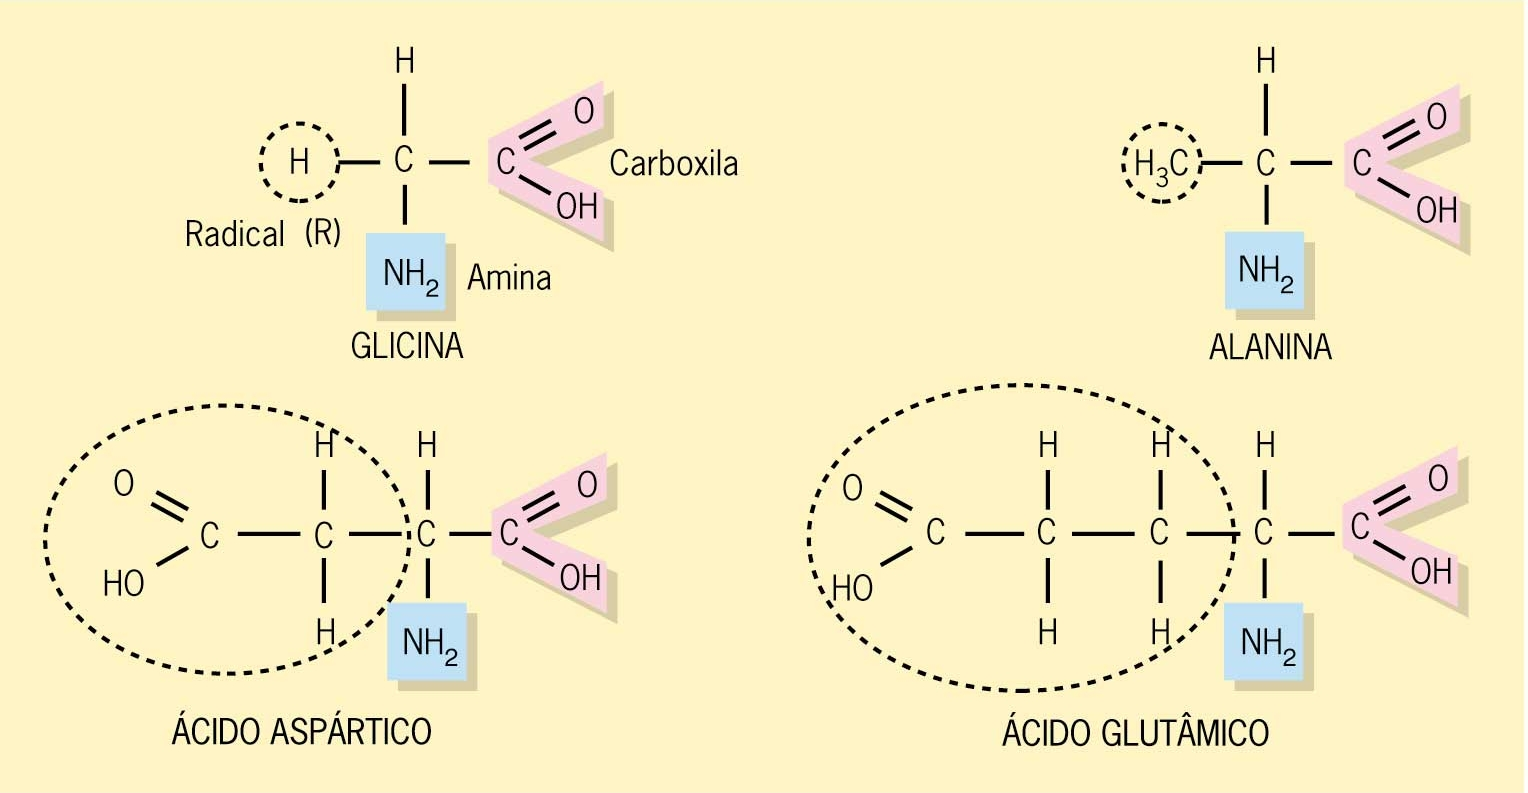
\includegraphics[scale=.2]{imgs/AminoacidosRadicais}
	\caption{Amino�cidos e seus radicais}
	Fonte: \cite{Junior:l03}
	\label{fgr:AminoacidosRadicais}
\end{figure}

Pode-se dividir os amino�cidos em dois tipos: os naturais e os essenciais. Os amino�cidos naturais s�o os que um organismo animal � capaz de produzir. Os amino�cidos essenciais s�o aqueles que os animais precisam ingerir, j� que s�o obrigat�rios para a s�ntese de suas prote�nas e para sua sobreviv�ncia. Os vegetais s�o capazes de produzir os vinte amino�cidos necess�rios conhecidos � produ��o de suas prote�nas \cite{Junior:l03}.

Dois amino�cidos se unem na m�lecula de prote�na atrav�s de uma liga��o pept�dica. Como ilustra a Figura \ref{fgr:LigacaoPeptidica} a rea��o ocorre entre a carboxila de um amino�cido e a amina de outro, havendo perda de uma mol�cula de �gua, trata-se de uma s�ntese por desidrata��o. O produto formado quando dois amino�cidos se ligam � chamado de dipept�deo, o tripept�deo e o tetrapept�deo s�o formados, respectivamente, por tr�s e quatro amino�cidos \cite{Nelson:l06}.

Quando ocorre um n�mero maior de amino�cidos na mol�cula, usa-se o termo polipept�deo, o termo prote�na � usado para designar pept�deos com n�mero superior a setenta amino�cidos \cite{Junior:l03, Nelson:l06}.

\begin{figure}[htp]
	\centering
	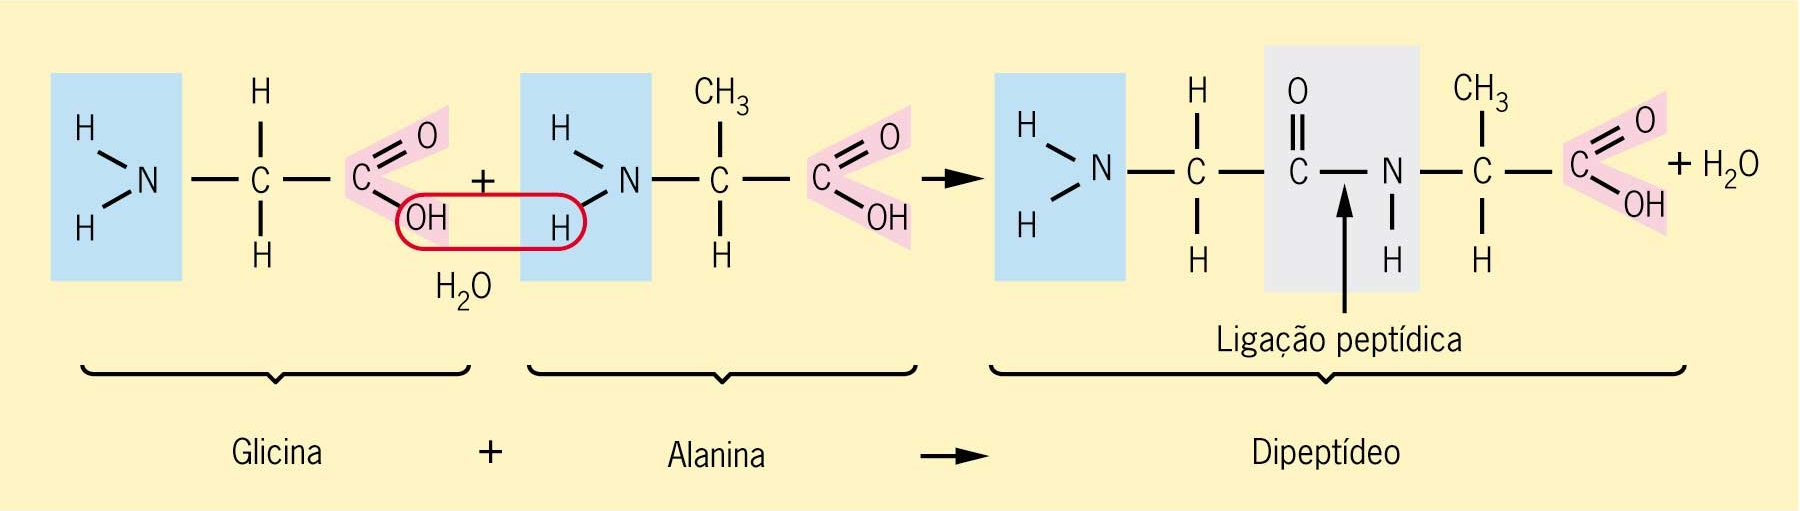
\includegraphics[scale=.2]{imgs/LigacaoPeptidica}
	\caption{Esquema de forma��o de um dipept�deo}
	Fonte: \cite{Junior:l03}
	\label{fgr:LigacaoPeptidica}
\end{figure}

Os amino�cidos s�o blocos formadores de prote�nas e tecido muscular. Todos os tipos de processo fisiol�gicos como energia, recupera��o, ganhos de m�sculos, for�a e perda de gordura, assim como fun��es do c�rebro e temperamento, est�o inteiramente ligados aos amino�cidos. Eles tamb�m podem ser convertidos e enviados diretamente para o ciclo de produ��o de energia do m�sculo \cite{Motta:l05, Nelson:l06}.

S�o 20 os amino�cidos construtores moleculares de prote�nas. De acordo com uma classifica��o aceita, nove s�o chamados de amino�cidos essenciais, significando que s�o fornecidos por algum alimento ou fonte de suprimento. E os demais, chamados amino�cidos dispens�veis ou condicionalmente indispens�veis, s�o baseado na habilidade do organismo em sintetiz�-los de outros amino�cidos \cite{Champe:l06}. Nas Tabelas \ref{tbl:AminoacidosEssenciais1} e \ref{tbl:AminoacidosEssenciais2} s�o apresentados os amino�cidos essenciais, com a sua abreviatura e fun��o.

\begin{table}[ht]
	\centering
	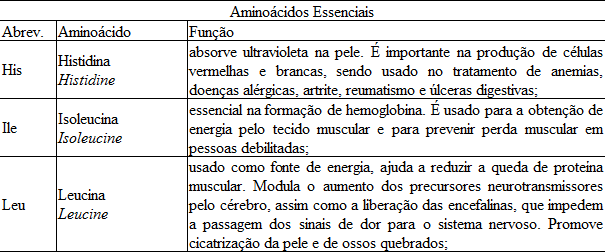
\includegraphics[width=1\textwidth]{imgs/AminoacidosEssenciais1}
	\caption{Amino�cidos essenciais (1/2)}
	\label{tbl:AminoacidosEssenciais1}
\end{table}

\begin{table}[ht]
	\centering
	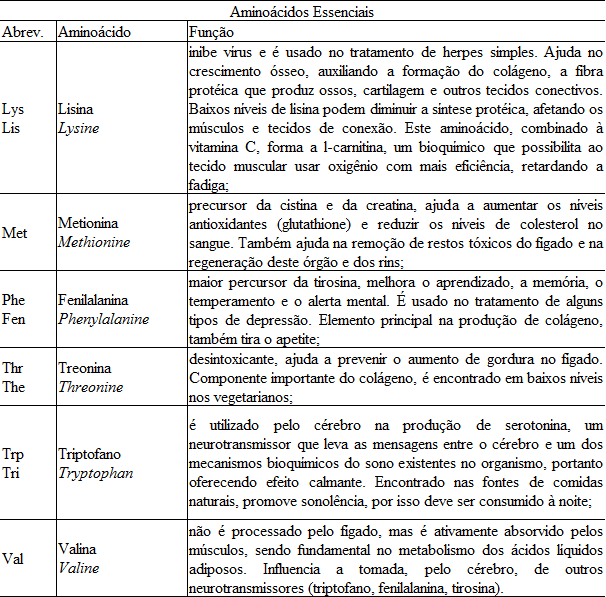
\includegraphics[width=1\textwidth]{imgs/AminoacidosEssenciais2}
	\caption{Amino�cidos essenciais (2/2)}
	\label{tbl:AminoacidosEssenciais2}
\end{table}

Logo ap�s, nas Tabelas \ref{tbl:AminoacidosDispensaveis1} e \ref{tbl:AminoacidosDispensaveis2} s�o apresentados os amino�cidos dispens�veis, com a sua abreviatura e fun��o. E, por fim, na Tabela \ref{tbl:AminoacidosCondicionalmenteIndispensaveis} s�o apresentados os amino�cidos condicionalmente indispens�veis, com a sua abreviatura e fun��o.

\begin{table}[htp]
	\centering
	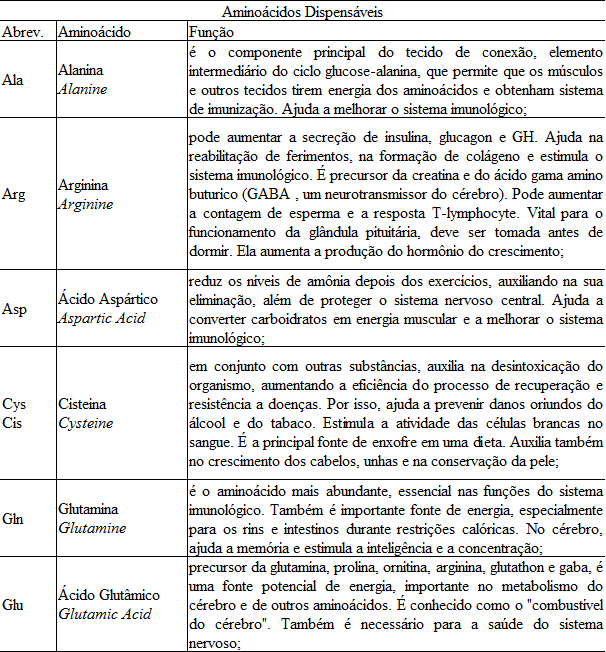
\includegraphics[width=1\textwidth]{imgs/AminoacidosDispensaveis1}
	\caption{Amino�cidos dispens�veis (1/2)}
	\label{tbl:AminoacidosDispensaveis1}
\end{table}

\begin{table}[htp]
	\centering
	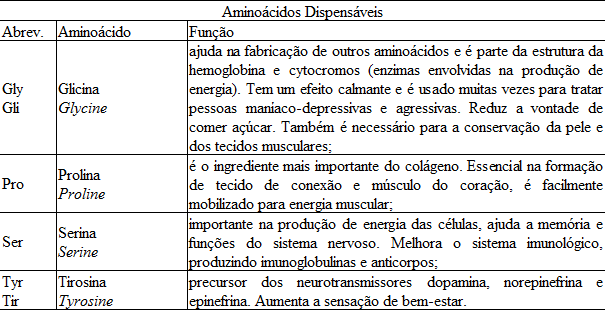
\includegraphics[width=1\textwidth]{imgs/AminoacidosDispensaveis2}
	\caption{Amino�cidos dispens�veis (2/2)}
	\label{tbl:AminoacidosDispensaveis2}
\end{table}

\begin{table}[htp]
	\centering
	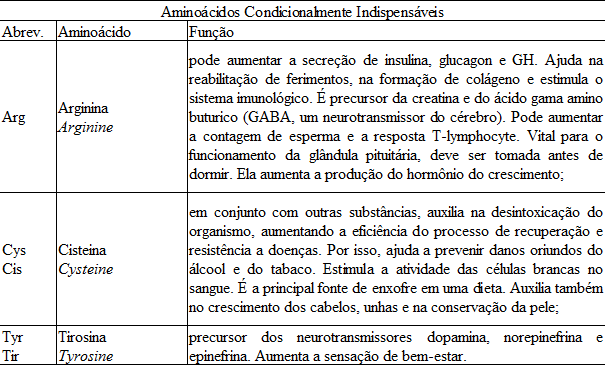
\includegraphics[width=1\textwidth]{imgs/AminoacidosCondicionalmenteIndispensaveis}
	\caption{Amino�cidos condicionalmente indispens�veis}
	\label{tbl:AminoacidosCondicionalmenteIndispensaveis}
\end{table}

\subsection{A estrutura da prote�na}

As prote�nas s�o constitu�das por apenas vinte tipos de amino�cidos conhecidos, mesmo assim, o n�mero de tipos de prote�nas existentes na natureza � extremamente grande. Al�m do n�mero de amino�cidos variar de setenta a alguns milhares, as diferentes seq��ncias que esses amino�cidos podem formar s�o praticamente infinitas \cite{Berg:l04, Junior:l03}.

\pagebreak

As prote�nas podem ser estudadas sobre dois enfoques, a constitui��o do fio prot�ico e a forma da mol�cula. A constitui��o do fio prot�ico trata dos tipos de amino�cidos que comp�em a prote�na, ou seja, quando estuda-se uma prote�na quanto aos tipos de amino�cidos que fazem parte dela e quanto � seq��ncia em que est�o ordenados, se esta analisando sua estrutura prim�ria. A seq��ncia exata dos amino�cidos numa prote�na � extremamente importante para o desempenho de sua fun��o, quando a c�lula, por motivos heredit�rios, comete enganos trocando um amino�cido por outro na seq��ncia de uma prote�na, pode alterar totalmente o funcionamento da prote�na, causando doen�as s�rias ou a prote�na fica sem fun��o e desaparece \cite{Junior:l03, Nelson:l06}.

A forma da mol�cula trata de como a cadeia de amino�cidos se torce, j� que as prote�nas n�o s�o fios esticados, formando uma h�lice, como um fio de telefone. Esse enovelamento na forma de uma h�lice representa o que os qu�micos chamam de estrutura secund�ria. E a pr�pria h�lice se torce sobre si mesma, adquirindo uma forma espacial arredondada. A forma definitiva da prote�na � determinada pelo modo como a h�lice se dobra e � chamada de estrutura terci�ria. Por raz�es qu�micas, a estrutura terci�ria depende da seq��ncia de amino�cidos, assim, prote�nas com seq��ncias diferentes t�m formas ou estruturas terci�rias tamb�m diferentes \cite{Berg:l04, Junior:l03}. A Figura \ref{fgr:EstruturaProteina} mostra as diferentes estruturas da prote�na.

\begin{figure}[htp]
	\centering
	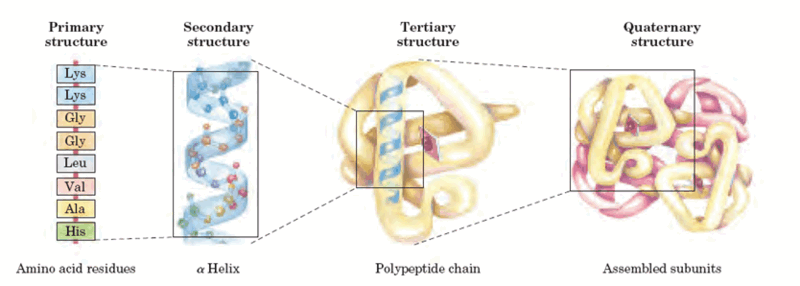
\includegraphics[scale=.5]{imgs/EstruturaProteina}
	\caption{Estrutura da prote�na}
	Fonte: \cite{Nelson:l06}
	\label{fgr:EstruturaProteina}
\end{figure}

\subsection{Prote�nas: rela��o entre forma e fun��o}

Em muitas prote�nas, a forma determina seu papel biol�gico, ou seja, prote�nas diferentes, tendo formas diferentes, apresentam atividade biol�gica diferente. Quando uma prote�na � submetida a certos tratamentos qu�micos, ou ent�o a temperaturas elevadas, ela se altera muitas vezes de forma permanente, o que � chamado de desnatura��o \cite{Junior:l03, Nelson:l06}.

Isso ocorre quando o tratamento empregado rompe certas liga��es qu�micas que mantinham a forma da mol�cula e quando as prote�nas celulares se deformam, elas perdem a capacidade de desempenhar suas fun��es \cite{Junior:l03}.

\section{O dogma central da biologia molecular}

O dogma central da biologia estabelece que o DNA atua como um modelo para se replicar, ele tamb�m � transcrito no RNA e o RNA � traduzido em prote�na, conforme ilustra a Figura \ref{fgr:DuplicacaoTranscricaoTraducao} \cite{Gibas:l01}.

\begin{figure}[htp]
	\centering
	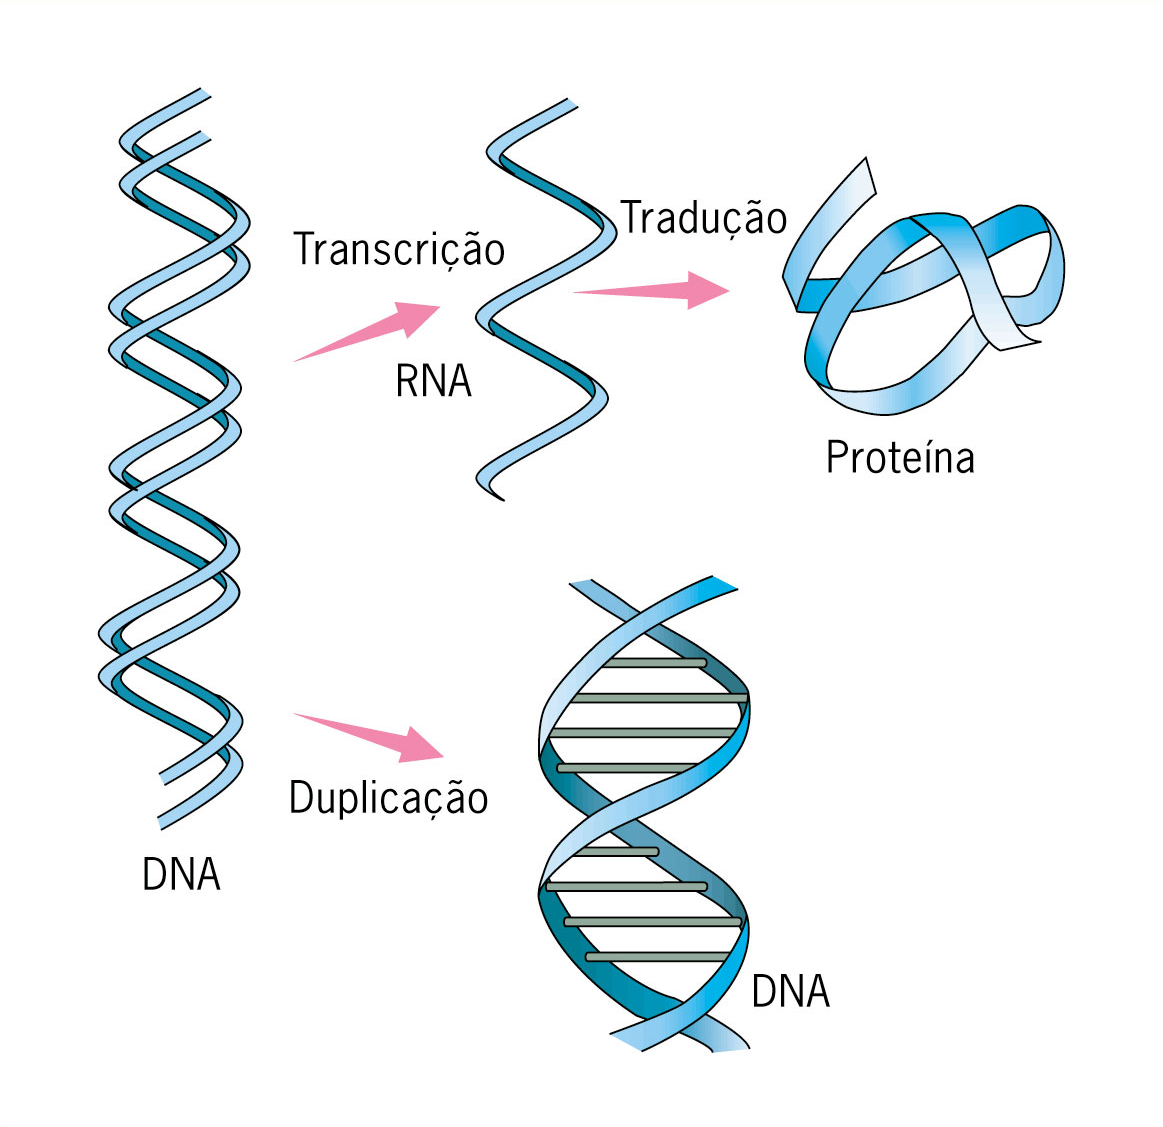
\includegraphics[scale=.19]{imgs/DuplicacaoTranscricaoTraducao}
	\caption{Duplica��o, transcri��o e tradu��o}
	Fonte: \cite{Junior:l03}
	\label{fgr:DuplicacaoTranscricaoTraducao}
\end{figure}

A informa��o gen�tica � conservada e passada para os descendentes por meio do processo de replica��o, e essas informa��es gen�ticas tamb�m s�o usadas pelo organismo individual por meio de processos de transcri��o e tradu��o \cite{Gibas:l01, Nelson:l06}.

O DNA gen�mico cont�m o plano mestre de um ser vivo e, sem ele, os organismos n�o seriam capazes de se auto-replicarem. A seq��ncia de DNA ``unidimensional'' � s� informa��o, que � lida pelo sistema de s�ntese da prote�na da c�lula \cite{Gibas:l01, Nelson:l06}.

\subsection{A estrutura do DNA e do RNA}

O DNA e o RNA s�o macromol�culas constitu�das por centenas ou milhares de nucleot�deos ligados entre si. Cada nucleot�deo � sempre composto por tr�s partes: um grupo fosfato (um a��car do grupo das pentoses), a desoxirribose (no caso do DNA) e uma base nitrogenada \cite{Junior:l03, Zaha:l01}. A Figura \ref{fgr:NucleotideosDNA} ilustra essa liga��o para os quatro diferentes tipos de nucleot�deos.

\begin{figure}[htp]
	\centering
	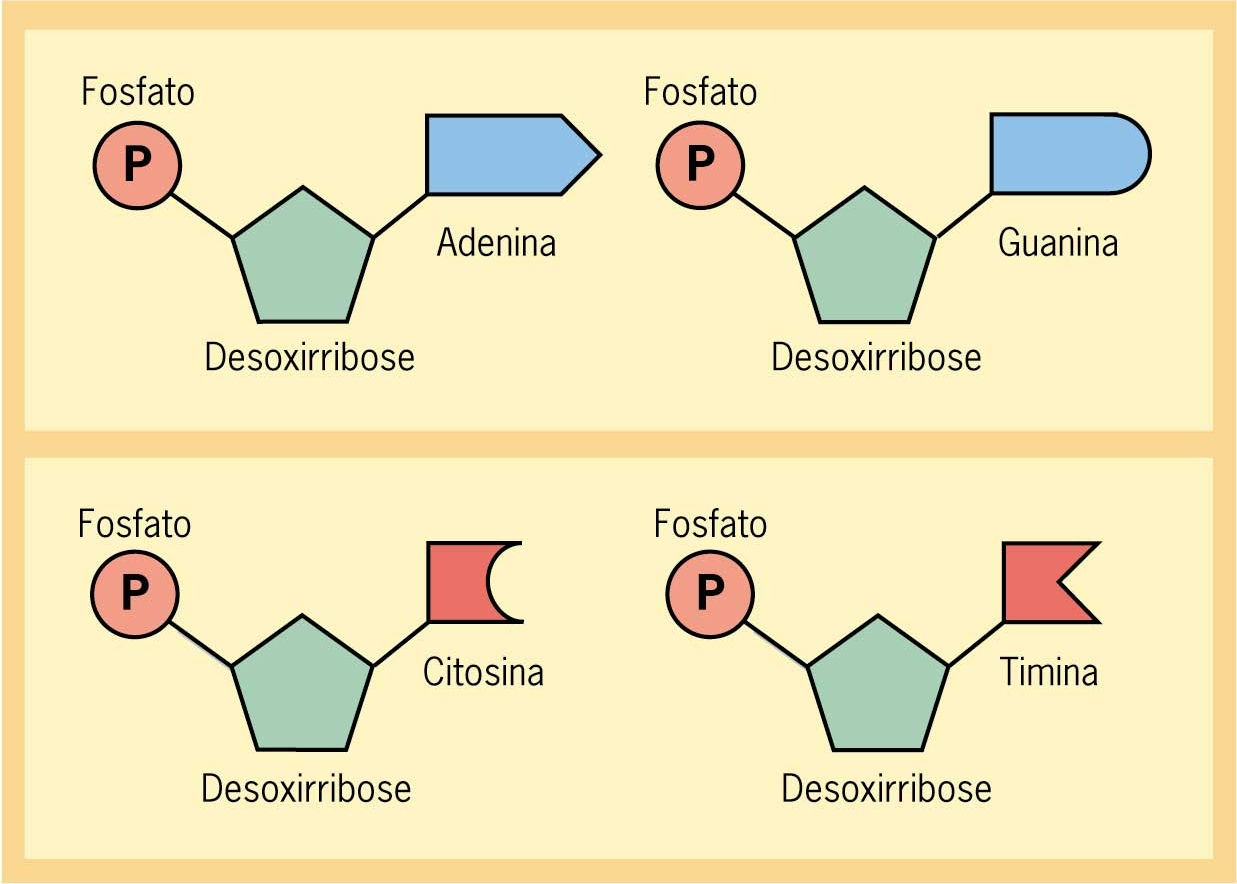
\includegraphics[scale=.18]{imgs/NucleotideosDNA}
	\caption{Nucleot�deos do DNA}
	Fonte: \cite{Junior:l03}
	\label{fgr:NucleotideosDNA}
\end{figure}

As bases nitrogenadas podem ser p�ricas, adenina e guanina ou pirim�dicas, citosina e timina, a base uracila, tamb�m pirim�dica, � encontrada somente no RNA. As bases p�ricas, maiores, s�o constitu�das de um anel duplo de carbono e nitrog�nio, enquanto que as pirim�dicas, menores, s�o compostas por um anel simples \cite{Berg:l04, Junior:l03, Zaha:l01}.

A mol�cula de DNA � constitu�da por duas cadeias de nucleot�deos e em cada cadeia, os nucleot�deos est�o ligados uns aos outros pelos fosfatos. Na mol�cula de DNA, as duas cadeias de nucleot�deos est�o ligadas uma � outra pelas suas bases nitrogenadas, por meio de pontes de hidrog�nio. Por motivos de configura��o molecular, a liga��o ocorre entre pares de bases espec�ficas, assim, a adenina liga-se a timina, e a citosina liga-se � guanina. A mol�cula de DNA assemelha-se, ent�o, a uma escada de corda: nela, fosfatos e pentoses representam os corrim�os, enquanto os degraus da escada s�o representados pelos pares de base \cite{Junior:l03, Paris:m08}. A Figura \ref{fgr:MoleculaDNA} ilustra o esquema de mol�cula de DNA.

\begin{figure}[htp]
	\centering
	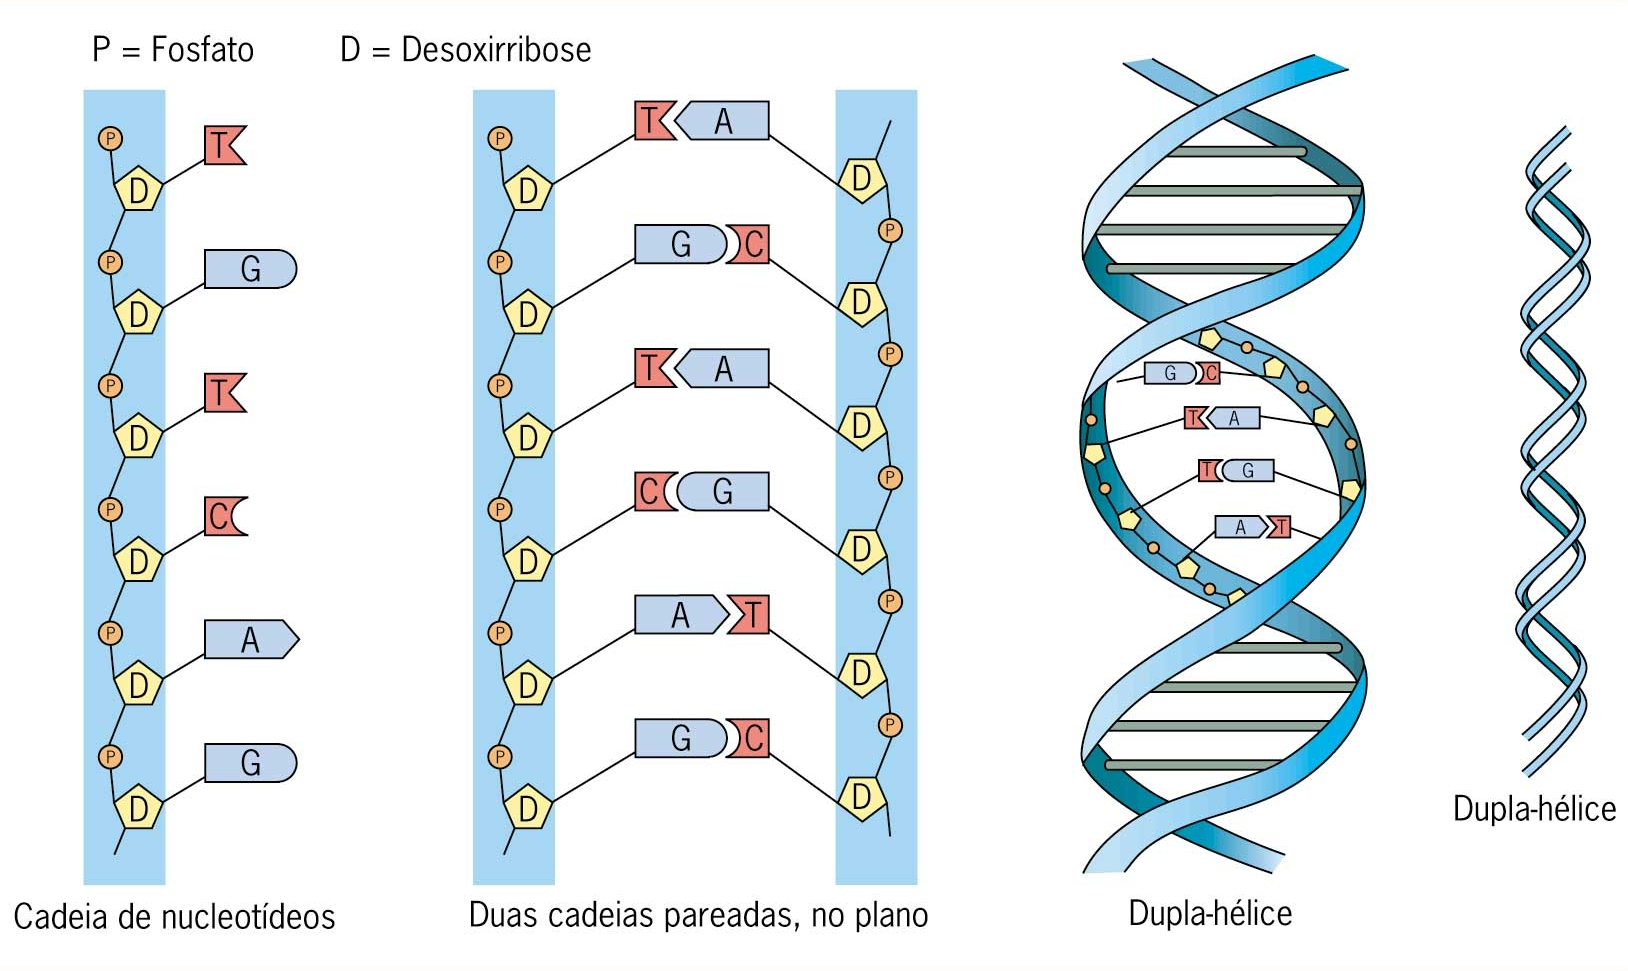
\includegraphics[scale=.23]{imgs/MoleculaDNA}
	\caption{Esquema de mol�cula de DNA}
	Fonte: \cite{Junior:l03}
	\label{fgr:MoleculaDNA}
\end{figure}

As estruturas do DNA e do RNA se diferem em tr�s aspectos: enquanto o DNA � formado por duas cadeias de nucleot�deos, o RNA � formado por uma fita �nica; a pentose no RNA � sempre a ribose (no DNA � a desoxirribose); e a uracila � exclusiva do RNA, da mesma forma que a timina caracteriza o DNA \cite{Berg:l04, Junior:l03, Zaha:l01}. A Figura \ref{fgr:MoleculaRNA} ilustra o esquema de mol�cula de RNA.

\begin{figure}[htp]
	\centering
	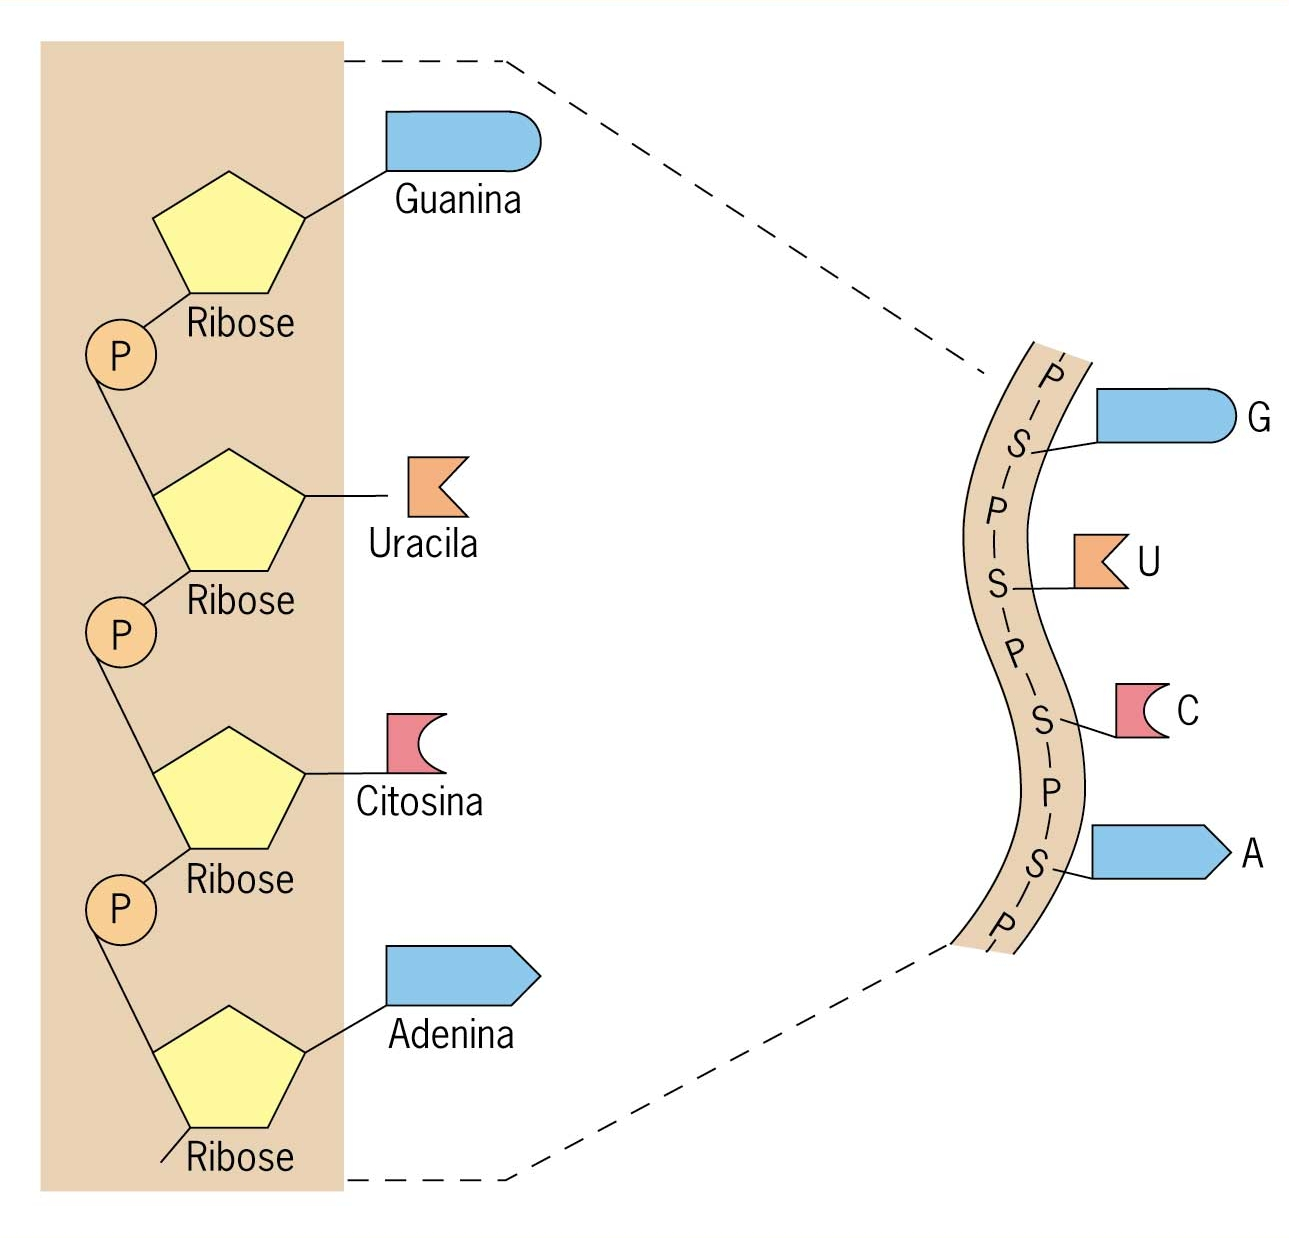
\includegraphics[scale=.23]{imgs/MoleculaRNA}
	\caption{Esquema de mol�cula de RNA}
	Fonte: \cite{Junior:l03}
	\label{fgr:MoleculaRNA}
\end{figure}

\subsection{Replica��o de DNA}

A especificidade do pareamento das bases sugere que cada uma das fitas parentais separadas pode atuar como molde para a s�ntese de uma fita-filha complementar \cite{Gibas:l01, Lewin:l01}. Isso � demostrado na Figura \ref{fgr:DuplicacaoDNA01} e o seu funcionamento ocorre da seguinte forma:

\begin{figure}[htp]
	\centering
	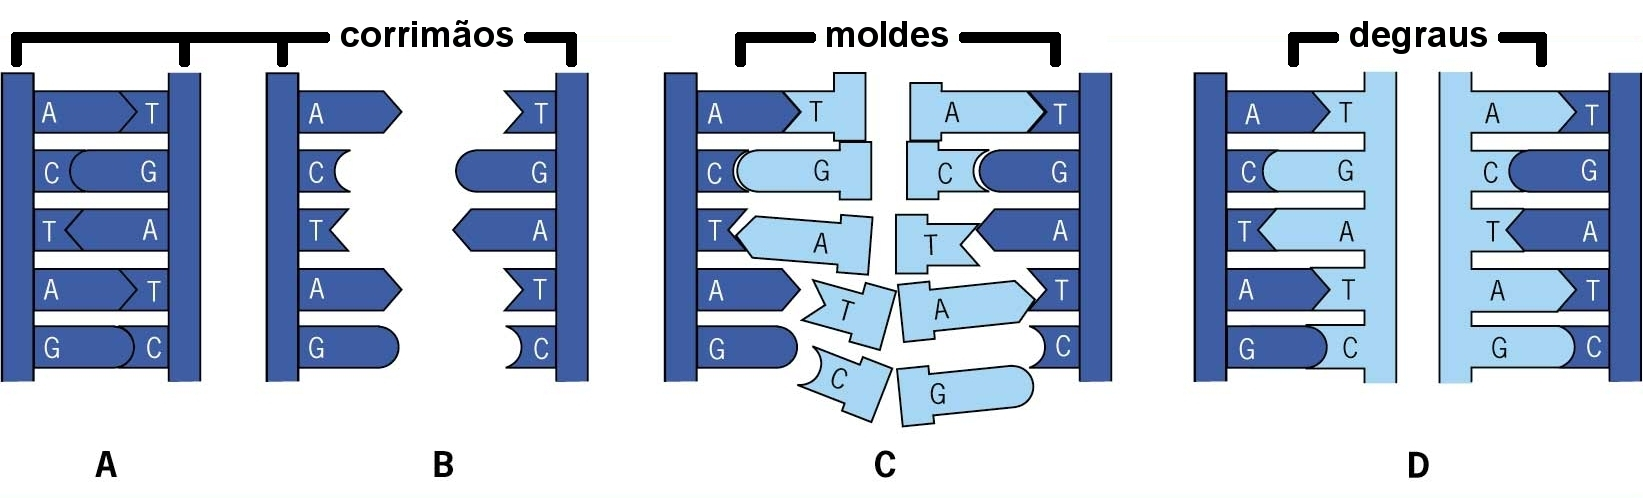
\includegraphics[scale=.2]{imgs/DuplicacaoDNA01}
	\caption{Esquema de duplica��o de DNA}
	Fonte: \cite{Junior:l03}
	\label{fgr:DuplicacaoDNA01}
\end{figure}

\begin{enumerate}
	\item[a)] Nessa etapa tem-se, duas fitas complementares de DNA em que as bases nitrogenadas est�o ligadas por pontes de hidrog�nio. Os ``corrim�os'' laterais s�o formados por fosfato e desoxiribose intercalados \cite{Junior:l03, Nelson:l06};
	\item[b)] No primeiro passo da duplica��o, ou replica��o, as pontes de hidrog�nio que ligam as bases nitrogenadas se rompem, e as duas fitas se separam \cite{Junior:l03, Zaha:l01};
	\item[c)] Cada uma das fitas originais (azul-escuro) serve de ``molde'' para a produ��o de fitas novas (azul-claro), que s�o formadas por nucleot�deos de DNA livres, que j� estavam presentes na c�lula. Os nucleot�deos novos tamb�m se ligam entre si, formando um novo ``corrim�o'', com a�ucar e fosfato alternados \cite{Gibas:l01, Junior:l03};
	\item[d)] Nessa etapa temos duas mol�culas de DNA id�nticas quanto a seq��ncia de pares de bases, de ``degraus''. Cada mol�cula, agora, tem uma fita velha (azul-escuro), que pertenceu � mol�cula original, e uma fita nova (azul-claro), rec�m-formada \cite{Junior:l03}.
\end{enumerate}

Para a duplica��o acontecer, s�o necess�rias v�rias enzimas, uma delas, a helicase que separa as duas h�lices, uma outra, a DNA polimerase que permite a liga��o de nucleot�deos novos ao molde de DNA \cite{Junior:l03}.

Esse processo de duplica��o em que cada mol�cula-filha conservou a metade da mol�cula-m�e, tamb�m � chamado de duplica��o semiconservativa \cite{Junior:l03, Lewin:l01, Nelson:l06}. A Figura \ref{fgr:DuplicacaoDNA02} ilustra em tr�s dimens�es o processo de duplica��o do DNA.

\begin{figure}[htp]
	\centering
	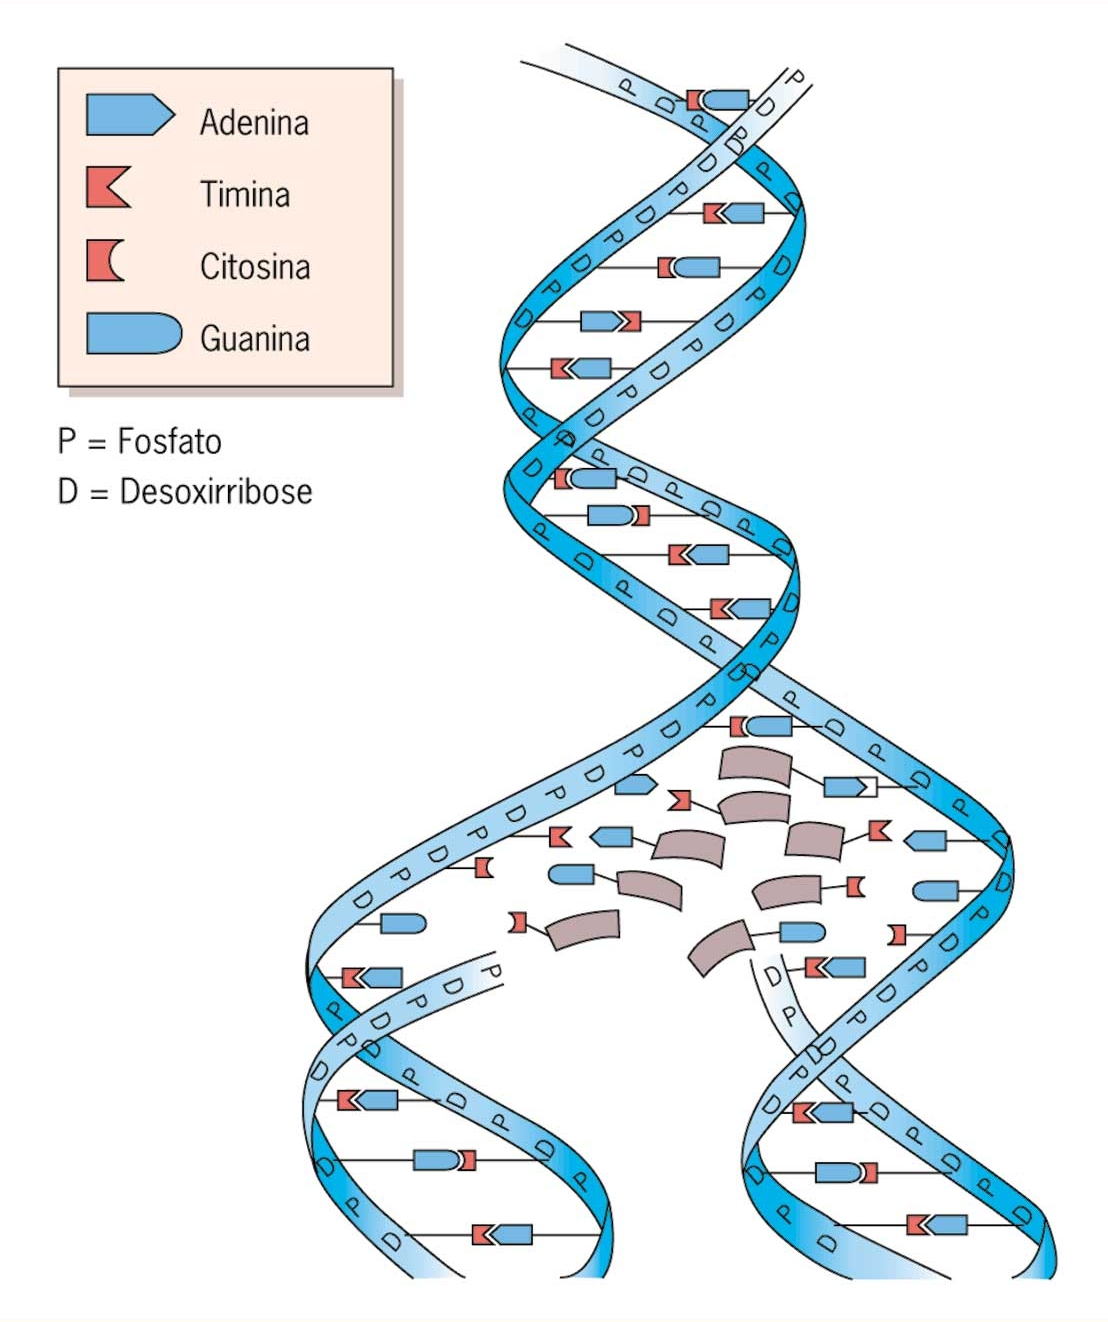
\includegraphics[scale=.2]{imgs/DuplicacaoDNA02}
	\caption{Duplica��o do DNA}
	Fonte: \cite{Junior:l03}
	\label{fgr:DuplicacaoDNA02}
\end{figure}

\subsection{Transcri��o de DNA}

O DNA n�o atua somente como um modelo para fazer c�pias de si mesmo, mas tamb�m como modelo para uma mol�cula chamada �cido ribonucl�ico (RNA) \cite{Gibas:l01, Lesk:l08, Nelson:l06}.

Enquanto a duplica��o, ou replica��o, � uma propriedade que permite a transmiss�o da informa��o gen�tica �s c�lulas-filhas, a produ��o de RNA relaciona-se � s�ntese de prote�nas, no citoplasma \cite{Junior:l03}. Isso � demostrado na Figura \ref{fgr:TranscricaoDNAtoRNA01} e o seu funcionamento ocorre da seguinte forma:

\begin{figure}[htp]
	\centering
	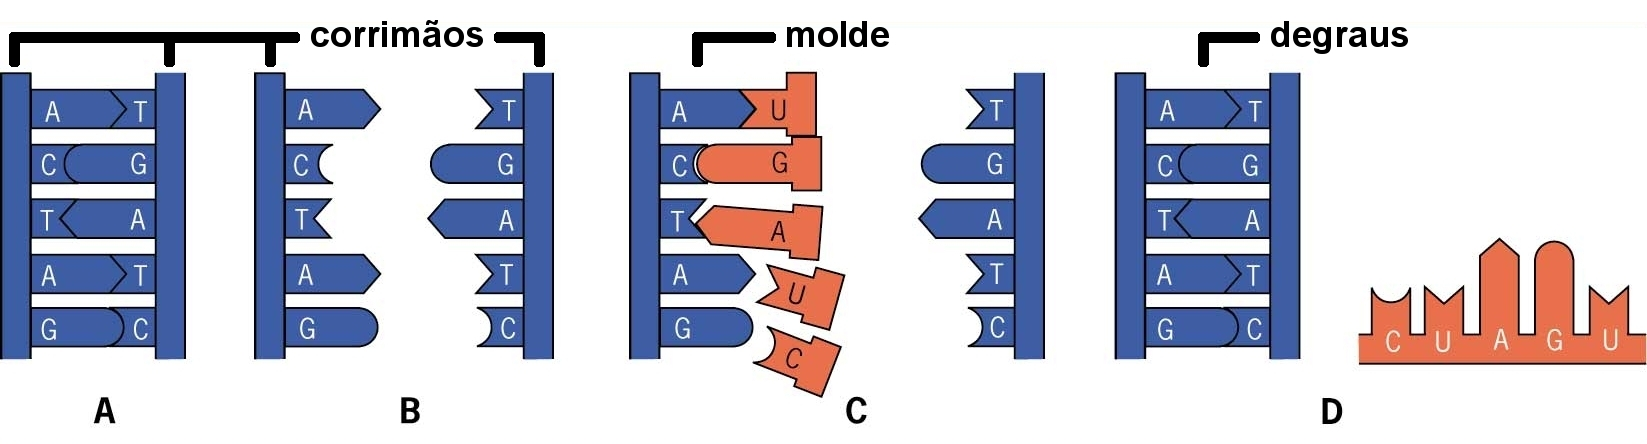
\includegraphics[scale=.2]{imgs/TranscricaoRNA01}
	\caption{Esquema de transcri��o de RNA}
	Fonte: \cite{Junior:l03}
	\label{fgr:TranscricaoDNAtoRNA01}
\end{figure}

\begin{enumerate}
	\item[a)] Nessa etapa temos um trecho de mol�cula de DNA, constitu�do por duas fitas complementares, cujas bases est�o ligadas entre si por pontes de hidrog�nio \cite{Junior:l03}.
	\item[b)] No primeiro passo da s�ntese de RNA, as pontes de hidrog�nio se rompem e as duas fitas se afastam uma da outra \cite{Junior:l03}. \pagebreak
	\item[c)] Apenas uma das fitas de DNA funciona como ``molde''. Nela, encaixam-se nucleot�deos de RNA j� existente na c�lula (em vermelho), que t�m a ribose como a��car. Repare que, na adenina do DNA, encaixa-se um nucleot�deo com a base uracila, exclusiva do RNA, em vez de timina, exclusiva do DNA. Os demais tipos de encaixe s�o semelhantes aos que ocorrem na replica��o do DNA. Enquanto isso, a segunda fita de DNA permanece inativa \cite{Junior:l03, Nelson:l06}.
	\item[d)] Uma vez produzida, a fita de RNA se destaca do ``molde'' de DNA e ir� migrar, mais tarde, para o citoplasma. Por fim, as duas fitas de DNA voltam a parear \cite{Junior:l03, Nelson:l06}.
\end{enumerate}

A mol�cula de RNA � uma fita simples e a informa��o para que ela seja produzida est� contida apenas numa das fitas do DNA, e n�o nas duas. Para o processo ocorrer, � necess�ria uma enzima especial chamada de RNA polimerase, que, al�m de afastar as fitas de DNA, permite o encaixe dos nucleot�deos de RNA \cite{Junior:l03}. A Figura \ref{fgr:TranscricaoDNAtoRNA02} ilustra em tr�s dimens�es o processo de transcri��o do DNA em RNA.

\begin{figure}[htp]
	\centering
	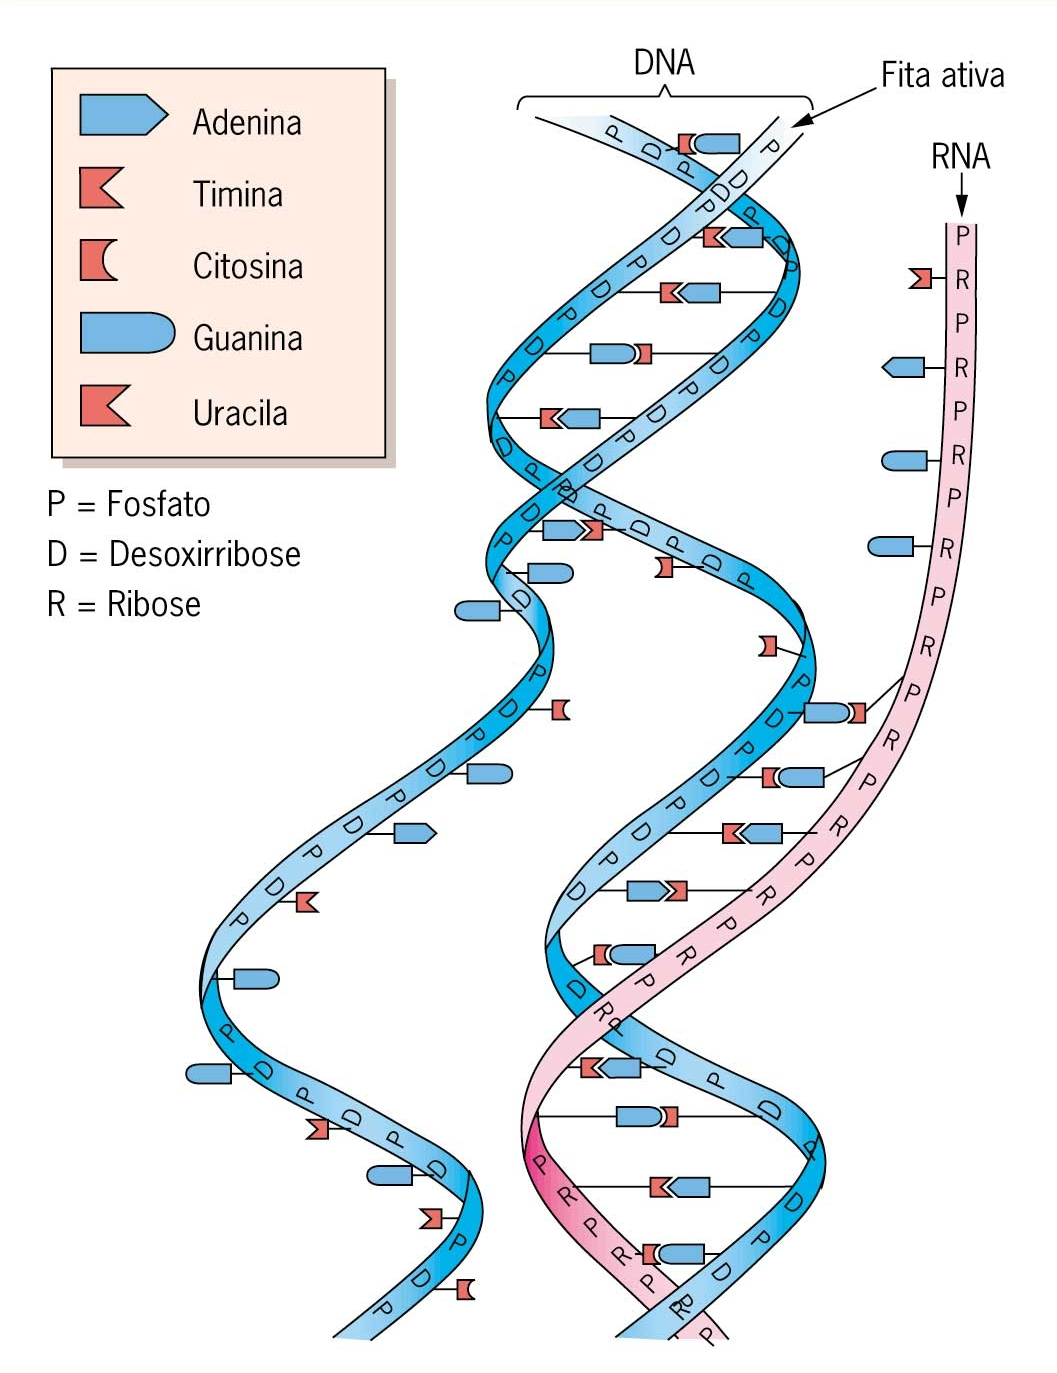
\includegraphics[scale=.2]{imgs/TranscricaoRNA02}
	\caption{Transcri��o de DNA em RNA}
	Fonte: \cite{Junior:l03}
	\label{fgr:TranscricaoDNAtoRNA02}
\end{figure}

O genoma fornece um modelo para a s�ntese de uma variedade de mol�culas de RNA, as tr�s principais s�o o RNA mensageiro, o RNA transportador e o RNA riboss�mico \cite{Gibas:l01, Lesk:l08}. 

As mol�culas de RNA mensageiro (mRNA) s�o transcritas do RNA dos genes, elas levam informa��es do genoma para o ribossomo, a maquin�ria de s�ntese prot�ica da c�lula. As mol�culas de RNA transportador (tRNA) s�o mol�culas de RNA n�o traduzidas que transportam amino�cidos, os blocos de constru��o das prote�nas, para os ribossomos. Finalmente, as mol�culas de RNA riboss�mico (rRNA) s�o os componentes de RNA n�o traduzido dos ribossomos, que s�o complexos de prote�nas e RNA. Os rRNA est�o envolvidos na fixa��o das mol�culas de mRNA e na cat�lise de algumas etapas no processo de tradu��o \cite{Gibas:l01}.

\subsection{Tradu��o de mRNA}

A tradu��o do mRNA em prote�na � a etapa final na coloca��o das informa��es contidas no genoma em funcionamento na c�lula. Como o DNA, as prote�nas s�o pol�meros lineares criados de um alfabeto de unidades quimicamente vari�veis, o alfabeto das prote�nas � um conjunto de pequenas mol�culas denominadas amino�cidos \cite{Gibas:l01, Lesk:l08}.

Ao contr�rio do DNA, a seq��ncia qu�mica de uma prote�na tem uma composi��o f�sico-qu�mico, assim como um conte�do informativo. Cada um dos 20 amino�cidos encontrados com mais freq��ncia nas prote�nas tem uma natureza qu�mica diferente, determinada por sua cadeia lateral (um grupo qu�mico que varia de amino�cido para amino�cido). A seq��ncia qu�mica da prote�na se chama estrutura prim�ria, mas a maneira pela qual a seq��ncia se dobra para formar uma mol�cula compacta � t�o importante para a fun��o da prote�na como � sua estrutura prim�ria. Os elementos das estruturas secund�ria e terci�ria que comp�em a dobra final da prote�na podem juntar partes distantes da seq��ncia qu�mica da prote�na para formar s�tios funcionais \cite{Gibas:l01, Nelson:l06}.

� correspond�ncia entre trincas de bases do DNA, trincas de bases do RNA e amino�cidos chamamos de c�digo gen�tico. Cada trinca de bases no DNA ou RNA � denominada c�don, essas trincas representam ``palavras'' do c�digo gen�tico e cada ``palavra'' corresponde a um ``objeto'', o amino�cido \cite{Junior:l03, Nelson:l06}.

Como mostra a Tabela \ref{fgr:CodigoGenetico}, o c�digo gen�tico � o c�digo que converte o DNA em prote�na. Ele utiliza tr�s bases de DNA (c�dons) para codificar cada amino�cido em uma seq��ncia de prote�na. As combina��es simples informam que h� 64 maneiras de selecionar 3 nucleot�deos de um conjunto de 4, portanto, h� 64 c�dons poss�veis e somente 20 amino�cidos \cite{Lesk:l08}.

Alguns c�dons s�o redundantes, outros t�m a fun��o especial de informar ao mecanismo de tradu��o da c�lula para parar de converter uma mol�cula de mRNA \cite{Gibas:l01}. A Figura \ref{fgr:CorrespondenciaEntreUnidade} mostra a correspond�ncia entre as unidades de DNA e do RNA e os amino�cidos da prote�na a ser sintetizada.

\begin{table}[htp]
	\centering
	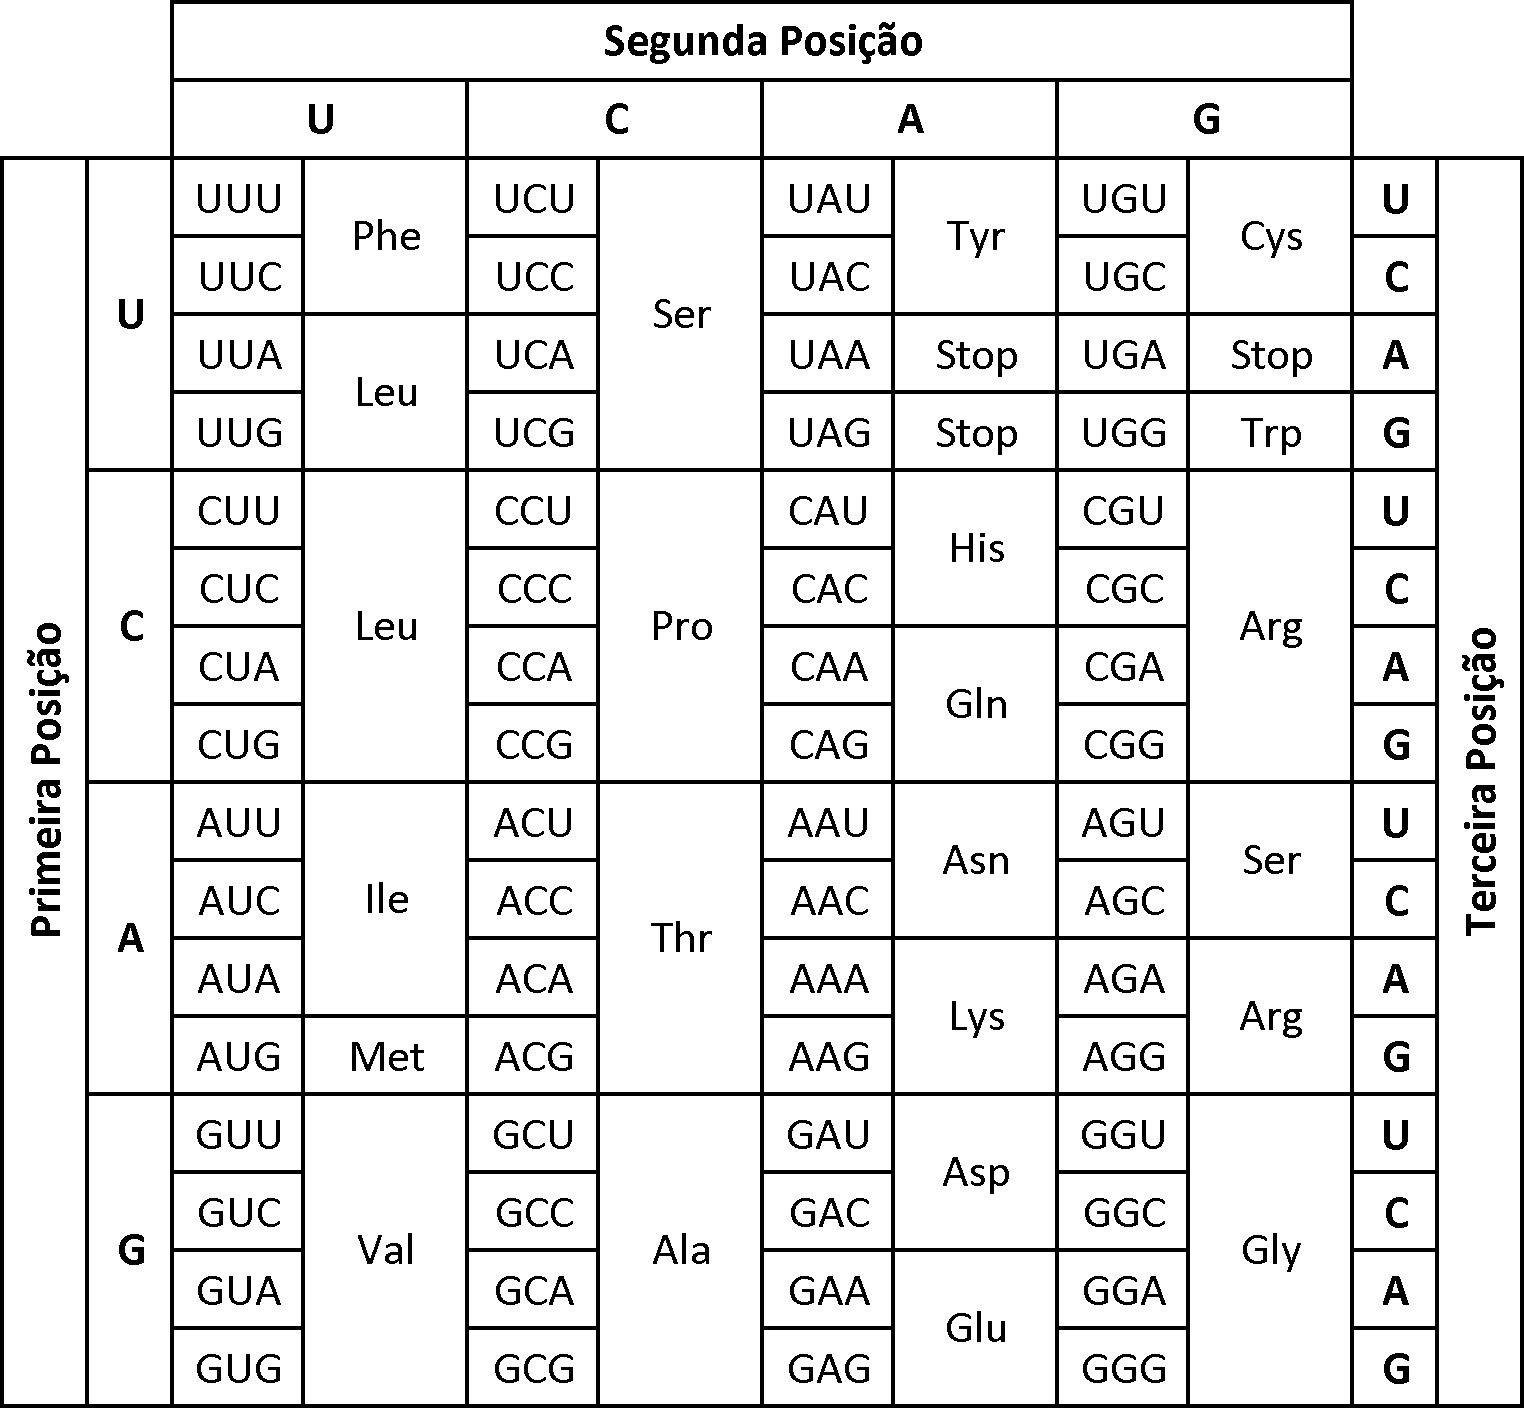
\includegraphics[scale=.85]{imgs/CodigoGenetico}
	\caption{C�digo gen�tico}
	Fonte: \cite{Gibas:l01}
	\label{fgr:CodigoGenetico}
\end{table}

\begin{figure}[htp]
	\centering
	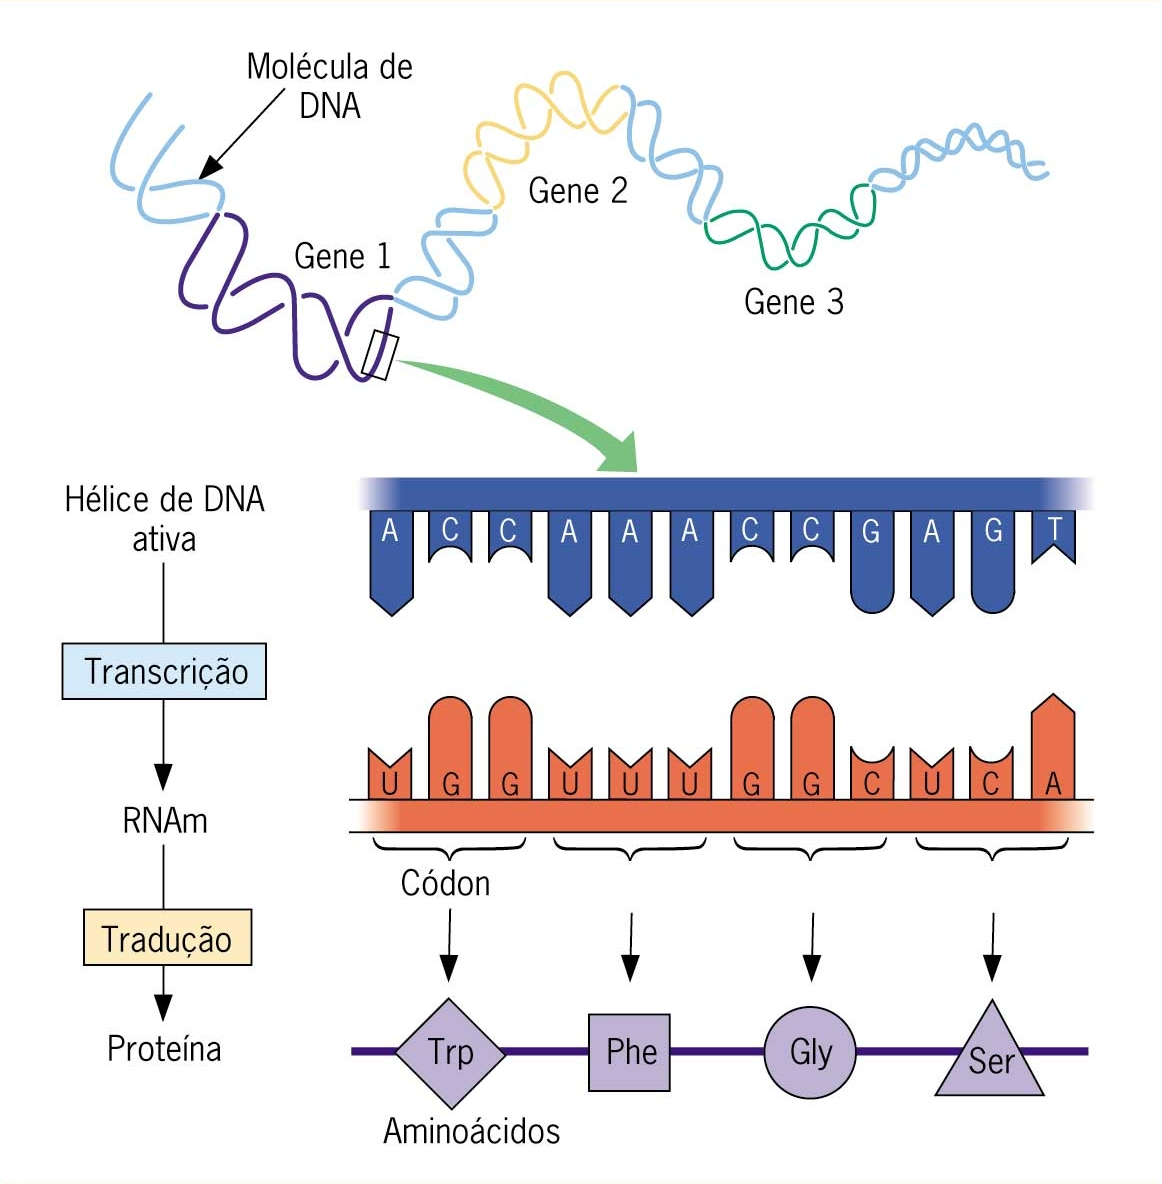
\includegraphics[scale=.23]{imgs/CorrespondenciaEntreUnidade}
	\caption{Correspond�ncia entre DNA, RNA e Amino�cidos}
	Fonte: \cite{Junior:l03}
	\label{fgr:CorrespondenciaEntreUnidade}
\end{figure}

\subsection{S�ntese de prote�nas}

Na Figura \ref{fgr:SinteseProteica} os amino�cidos foram representados em vermelho, como bolinhas, tri�ngulos, etc., para melhor ilustrar a explica��o.

\begin{figure}[htp]
	\centering
	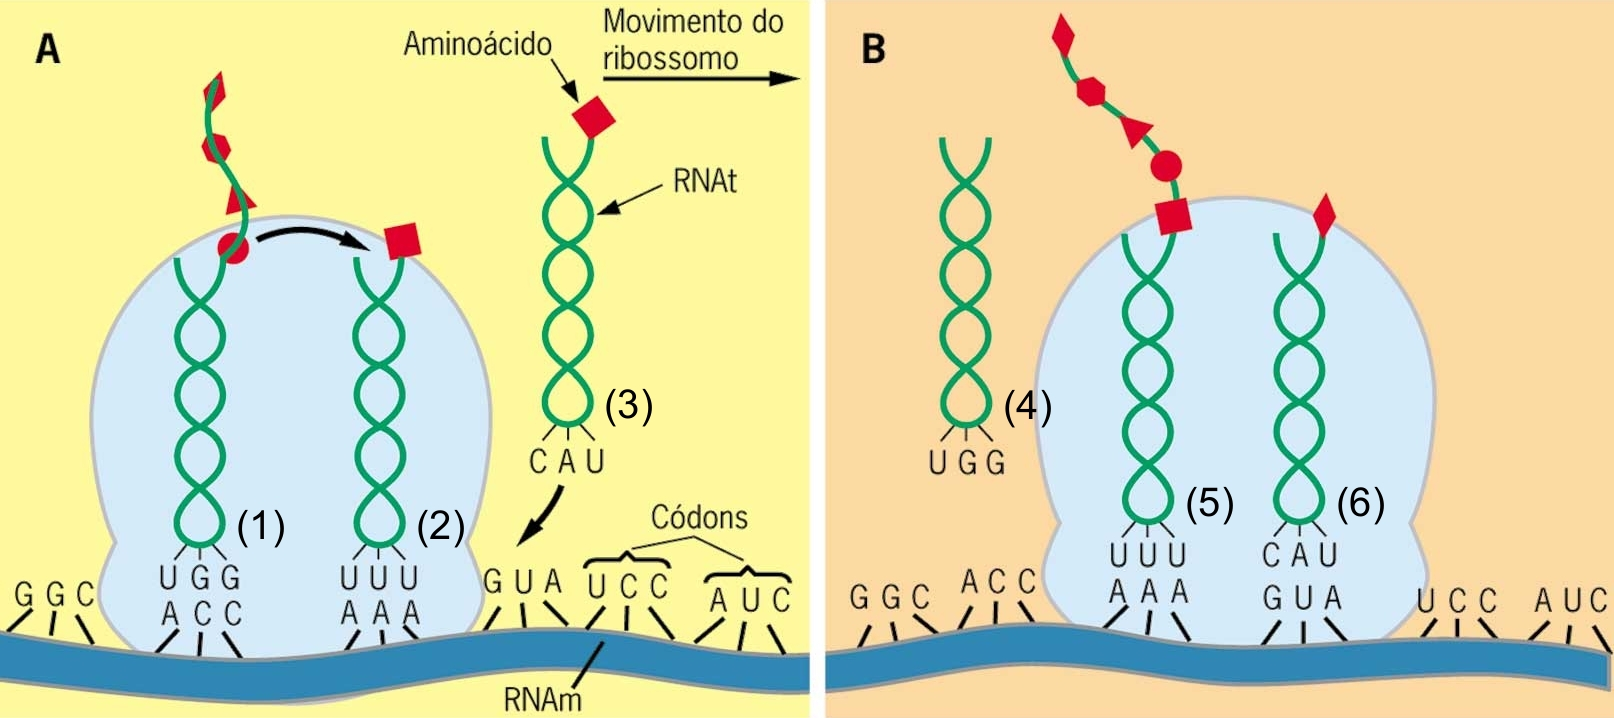
\includegraphics[scale=.23]{imgs/SinteseProteica}
	\caption{S�ntese prot�ica}
	Fonte: \cite{Junior:l03}
	\label{fgr:SinteseProteica}
\end{figure}

O ribossomo do esquema A (azul) desliza ao longo da fita de mRNA, movendo-se da esquerda para direita, no momento ele abrange dois c�dons do mRNA. O tRNA com o antic�don UGG (1) est� ligado � cadeia de amino�cidos, o segundo tRNA com o antic�don UUU (2), encaixa-se no c�don AAA (2) do mRNA e est� trazendo o amino�cido ``quadradinho''. Entre os amino�cidos ``bolinha'', o �ltimo da cadeia a ser fabricado, e ``quadradinho'', que acaba de ser trazido, vai se formar uma liga��o pept�dica \cite{Junior:l03, Nelson:l06}.

No esquema B � exemplificado o que ocorre na seq��ncia, a liga��o pept�dica entre os amino�cidos completou-se, e a cadeia polipept�dica foi acrescida de um amino�cido. O tRNA com o antic�don UGG (4) ent�o desliga-se da cadeia de amino�cidos e volta para o citoplasma, podendo buscar um novo amino�cido ``bolinha''. A prote�na em forma��o est� ligada agora ao tRNA com o antic�don UUU (5), o ribossomo deslizou para a direita, abrangendo um novo c�don do mRNA, GUA (6). O tRNA com o antic�don CAU (6), o �nico que pode se encaixar, est� trazendo o amino�cido ``losango''. Logo haver� liga��o pept�dica entre ``quadrinho'' e ``losango'' e o pen�ltimo tRNA, UUU (5), se desligar�, o ribossomo deslizar� para a direita, abrangendo mais um c�don, e assim por diante \cite{Junior:l03}.

A cada c�don que o ribossomo abrange, � acrescentado um amino�cido espec�fico � prote�na em crescimento, quando o ribossomo tiver percorrido todo o mRNA, toda a mensagem ter� sido lida e a prote�na estar� pronta. Ent�o o ribossomo se desliga do mRNA. A mesma fita de RNA pode ser lida por v�rios ribossomos e cada um deles produzir� uma mol�cula de prote�na exatamente igual \cite{Junior:l03, Nelson:l06}.

\subsection{Genomas e genes}

A seq��ncia completa de DNA que codifica um ser vivo � chamada de genoma, mas o genoma n�o funciona como uma seq��ncia longa, ele � dividido em genes individuais \cite{Gibas:l01}. Um gene � uma seq��ncia de DNA necess�ria para a s�ntese de uma prote�na, por�m existem ao longo dos cromossomos algumas seq��ncias de DNA especializadas capazes de transcrever, mas que n�o cont�m informa��o para a s�ntese de prote�na \cite{Junior:l03}.

Existem tr�s tipos de genes. Os genes codificadores de prote�nas s�o modelos para gerar mol�culas de prote�nas. Cada prote�na codificada pelo genoma � uma m�quina qu�mica com um prop�sito distinto no organismo. Os genes especificadores de RNA tamb�m s�o modelos para as m�quinas qu�micas, mas os blocos criadores das m�quinas de RNA s�o diferentes dos que comp�em a prote�na. E, por fim, os introns (genes n�o transcritos) s�o regi�es do DNA gen�mico que possuem algum prop�sito funcional, mas n�o alcan�am esse prop�sito, sendo transcritos ou convertidos para criar outra mol�cula \cite{Gibas:l01, Lesk:l08}.

\subsection{Evolu��o molecular}

Os erros na replica��o e transcri��o de DNA s�o relativamente comuns. Se esses erros ocorrem nas c�lulas reprodutoras de um organismo, eles podem ser transmitidos aos seus descendentes. As altera��es na seq��ncia de DNA s�o conhecidas como muta��es, e essas muta��es podem ter resultados prejudiciais, resultados que diminuem a probabilidade de sobreviv�ncia dos descendentes at� a idade adulta, resultados ben�ficos ou ser neutras. Se uma muta��o n�o mata o organismo antes que ele se reproduza, a muta��o pode se fixar na popula��o depois de muitas gera��es, a lenta acumula��o dessas mudan�as � respons�vel pelo processo conhecido como evolu��o \cite{Gibas:l01, Junior:l03}.

O acesso as seq��ncias de DNA permite o acesso a um melhor entendimento da evolu��o. Nosso entendimento do mecanismo de evolu��o molecular como um processo gradual de acumula��o de muta��es de seq��ncias de DNA � a justificativa para o desenvolvimento de hip�teses baseadas na compara��o das seq��ncias de DNA e de prote�nas \cite{Gibas:l01}.

\section{Bancos de dados biol�gicos}

Nas subse��es que seguem ser� comentada um pouco da hist�ria e qual a fun��o de alguns dos principais bancos de dados biol�gicos existentes.

\subsection{DDBJ}

O DDBJ\footnote{DDBJ - DNA Data Bank of Japan. Dispon�vel em: $<$\url{http://www.ddbj.nig.ac.jp}$>$. Acesso em: 14 de maio de 2009} (\emph{DNA Data Bank of Japan}) iniciou suas atividades em banco de dados de DNA em 1986 no \emph{National Institute of Genetics} (NIG), com o aval do Minist�rio da Educa��o, Ci�ncia, Esporte e Cultura. Desde o in�cio, o DDBJ tem funcionado com uma das bases de dados internacional de DNA, que inclui EBI (\emph{European Bioinformatics Institute}, respons�vel pela base de dados EMBL) na Europa e NCBI (\emph{National Center for Biotechnology Information}, respons�vel pela base de dados GenBank) nos Estados Unidos da Am�rica como os dois outros membros. Conseq�entemente o DDBJ tem colaborado com os outros dois bancos de dados atrav�s do interc�mbio de dados e informa��es pela Internet e pela sua regular participa��o nas duas reuni�es, a \emph{International DNA Data Banks Advisory Meeting} e a \emph{International DNA Data Banks Collaborative Meeting}.

O \emph{Center for Information Biology} no NIG foi reorganizado como o \emph{Center for Information Biology and DNA Data Bank of Japan} (CIB-DDBJ) em 2001. O novo centro desempenha um papel importante na realiza��o de projetos de investiga��o em informa��es biol�gicas. O DDBJ � o �nico banco de dados de DNA no Jap�o que � oficialmente certificado para recolher seq��ncias de DNA de pesquisadores, e de emitir o n�mero reconhecido internacionalmente para ades�o dos dados fornecidos. O DDBJ coleta dados principalmente de pesquisadores japoneses, mas evidentemente tamb�m aceita dados e emiti o n�mero de ades�o aos investigadores em todos os outros pa�ses. A troca de dados coletados entre a EMBL, EBI e GenBank, NCBI em uma base di�ria, proporciona que o os tr�s bancos partilhem de praticamente os mesmos dados em um determinado momento. O CIB-DDBJ tamb�m fornece muitas ferramentas para a recupera��o de dados e an�lises desenvolvidas atrav�s do DDBJ.

\subsection{EMBL-EBI}

O EBI\footnote{EMBL-EBI. Dispon�vel em: $<$\url{http://www.ebi.ac.uk}$>$. Acesso em: 30 de abril de 2009} (\emph{European Bioinformatics Institute}) � parte integrante do EMBL (\emph{European Molecular Biology Laboratory}). O EMBL-EBI foi o primeiro banco de dados do mundo de seq��ncia nucleot�dica tendo surgido em 1980 em Heidelberg, na Alemanha. O que come�ou com uma modesta tarefa de abstrair informa��es da literatura, logo se tornou uma importante base de dados com necessidade de pessoal altamente qualificado em inform�tica com o in�cio do projeto genoma. Seus grupos de investiga��o visam compreender a biologia atrav�s do desenvolvimento de novas abordagens para a interpreta��o dos dados biol�gicos.

\subsection{GenBank}

O GenBank\footnote{GenBank at NCBI. Dispon�vel em: $<$\url{http://www.ncbi.nlm.nih.gov/Genbank}$>$. Acesso em: 14 de maio de 2009} � um banco de dados de seq��ncias gen�ticas e uma cole��o de todas as anota��es de seq��ncias de DNA dispon�veis. Essa base cont�m aproximadamente 85.759.586.764 bases em 82.853.685 registros de seq��ncias. Os lan�amentos de novas vers�es s�o feitos a cada dois meses. O GenBank � parte do \emph{International Nucleotide Sequence Database Collaboration}, que inclui o {DNA DataBank} do Jap�o (DDBJ), o \emph{European Molecular Biology Laboratory} (EMBL) e o GenBank do NCBI.

A base de dados do GenBank � projetada para proporcionar e incentivar o acesso pela comunidade cient�fica a mais atualizada e completa seq��ncia de informa��es de DNA.
O NCBI est� continuamente desenvolvendo novas ferramentas e atualizando as j� existentes para melhorar a apresenta��o e o acesso ao GenBank. O NCBI n�o coloca restri��es � utiliza��o ou distribui��o dos dados do GenBank.

\subsection{OMIM}

OMIM\footnote{OMIM - Online Mendelian Inheritance in Man. Dispon�vel em: $<$\url{http://www.ncbi.nlm.nih.gov/omim}$>$. Acesso em: 24 de abril de 2009} (\emph{Online Mendelian Inheritance in Man}) � um cat�logo de atualiza��o cont�nua de genes humanos e doen�as gen�ticas (que � o seu principal foco), com \emph{links} para literaturas de refer�ncia, seq��ncias de registros, mapas, dados e afins. OMIM est� baseado no texto \emph{Mendelian Inheritance in Man}, de autoria do Dr. Victor A. McKusick e uma equipe de redatores e editores cient�ficos no John Hopkins University e da popula��o.

Esta base de dados foi iniciada no in�cio dos anos de 1960 pelo Dr. Victor A. McKusick com um cat�logo de tra�os mendelianos e transtornos, intitulado \emph{Mendelian Inheritance in Man} (MIM). Doze edi��es do livro foram publicadas entre 1966 e 1998. A vers�o online, OMIM, foi criada em 1985 por uma colabora��o entre a \emph{National Library of Medicine} e o \emph{William H. Welch Medical Library} em Johns Hopkins e em 1987 foi disponibilizada na Internet. Em 1995, OMIM foi desenvolvido para \emph{World Wide Web} pelo NCBI (\emph{National Center for Biotechnology Information}).

\subsection{PDB}

O PDB\footnote{PDB - Protein Data Bank. Dispon�vel em: $<$\url{http://www.rcsb.org/pdb/home/home.do}$>$. Acesso em: 14 de maio de 2009} (\emph{Protein Data Bank}) � o �nico reposit�rio de informa��es sobre as estruturas 3D de grandes mol�culas biol�gicas, incluindo prote�nas e �cidos nucl�icos. Compreender a forma de uma mol�cula ajuda a compreender como ela funciona, esse conhecimento pode ser usado para ajudar a deduzir o seu papel na estrutura da sa�de humana e doen�a, e desenvolvimento de drogas.

O PDB foi criado em 1971 no \emph{Brookhaven National Laboratory} e inicialmente continha sete estruturas. Em 1998, o \emph{Research Collaboratory for Structural Bioinformatics} (RCSB) ficou respons�vel pela gest�o do PDB. Em 2003, o wwPDB foi formado para manter um �nico arquivo do PDB de estruturas de dados macromoleculares que � livre e publicamente dispon�veis para a comunidade global. O wwPDB � constitu�do por organiza��es que atuam como deposi��o, processamento de dados e centros de distribui��o para os dados PDB. Al�m disso, o RCSB PDB suporta um \emph{site} onde os visitantes podem realizar consultas simples e complexas sobre os dados, analisar e visualizar os resultados. O RCSB PDB est� localizado na Rutgers, \emph{The State University of New Jersey} e na \emph{University of California}, San Diego.

O RCSB PDB � um membro da wwPDB, um esfor�o de colabora��o com PDBe (Reino Unido), PDBj (Jap�o), e BMRB (E.U.A.) para assegurar que o arquivo PDB seja global e uniforme. O PDB arquivo est� dispon�vel sem nenhum custo para os utilizadores e novas estruturas s�o liberadas semanalmente.

\subsection{STRING}

STRING\footnote{STRING. Dispon�vel em: $<$\url{http://string.embl.de}$>$. Acesso em: 30 de abril de 2009} � uma base de dados em que constam intera��es de prote�nas conhecidas e previs�veis, essas intera��es podem ser associa��es diretas (f�sicas) e indiretas (funcionais) e s�o provenientes de quatro fontes: contexto gen�mico, experimentos, coexpress�o e conhecimentos pr�vios.

\subsection{Swiss-Prot}

O Swiss-Prot\footnote{Swiss-Prot. Dispon�vel em: $<$\url{http://www.expasy.ch/sprot}$>$. Acesso em: 14 de maio de 2009} � um banco de dados de seq��ncia de prote�nas que se empenha em oferecer um elevado n�vel de anota��o (como a descri��o da fun��o de uma prote�na, suas estruturas de dom�nios, variantes, etc.), um n�vel m�nimo de redund�ncia e um alto n�vel de integra��o com outras bases de dados. Esse banco de dados � desenvolvido pelo \emph{Swiss-Prot group} no \emph{Swiss Institute of Bioinformatics} (SIB) e no \emph{European Bioinformatics Institute} (EBI).

\section{Considera��es finais}

Nesse cap�tulo foi explicado a fun��o das prote�nas e o dogma central da biologia molecular, tamb�m foram apresentados alguns exemplos de reposit�rios de informa��es biol�gicas, quando poss�vel, dando �nfase ao conte�do que eles disponibilizam. No pr�ximo cap�tulo ser� apresentado o fluxo de pesquisa de uma doen�a g�nica, que � o foco desse trabalho, e ser� feita uma abordagem mais voltada para a �rea de biologia de sistemas.
	\chapter{Biologia de sistemas}

Ap�s o Projeto Genoma Humano ter completado sua fase inicial, cientistas e pol�ticos come�aram a articular cada vez mais, vis�es de como a tecnologia orientada para a aquisi��o de conhecimento gen�mico poderia ser transformada em estrat�gias de interven��o. A �rea em que muitas destas ambi��es e esperan�as convergiram � agora o que � chamado de biologia de sistemas. O objetivo global da biologia de sistemas � o objetivo final da biologia moderna, a obten��o de uma fundamental, abrangente e sistem�tica compreens�o da vida. Para atingir esta meta, existe a inten��o de integrar sistemas de bi�logos para obter uma explica��o global para DNA, RNA, prote�nas e dados metab�licos, combinando modelagem matem�tica e uma extensa an�lise computacional \cite{Malley:a05}.

A biologia de sistema n�o prev� transformar as compreens�es e pr�ticas dos bi�logos, mas os seus m�todos e conceitos prev�em ter efeitos importantes sobre outras ci�ncias, como f�sica, engenharia, matem�tica e ci�ncias sociais. Existem fortes argumentos que a biologia de sistemas � mais do que apenas uma extens�o do genoma e da bioinform�tica, ela � qualitativamente diferente do que j� foi alcan�ado e achado pelas ferramentas atuais \cite{Malley:a05}.

Nas se��es que seguem ser� apresentado um cen�rio exemplo de aplica��o em biologia de sistemas, a possibilidade de an�lise de uma doen�a atrav�s de redes de intera��o de prote�nas e o particionamento dos processos biol�gicos atrav�s da ontologia g�nica.

\section{Redes de livre-escala}

Uma rede (grafo) � uma cole��o de pontos aonde estes pontos s�o chamados de nodos ou v�rtices, e os arcos que conectam estes pontos s�o chamados de arestas. Redes biol�gicas, representa��es de relacionamentos biol�gicos, s�o constru�das para descrever v�rios fen�menos biol�gicos. Estas redes variam desde redes que descrevem condutores bioqu�micos da c�lula at� redes de mais alto n�vel tais como redes de neur�nios \cite{Bebek:a07}. 

A conduta de muitos sistemas complexos, das c�lulas a Internet, emerge de uma atividade orquestrada de muitos componentes que interagem com outros atrav�s de intera��es aos pares. Em um n�vel abstrato muito alto, os componentes podem ser reduzidos para uma s�rie de nodos que s�o conectados por liga��es que representam as intera��es entre dois componentes. Os nodos e liga��es juntos formam uma rede, ou, em uma linguagem matem�tica formal, um grafo \cite{Barabasi:a04}.

Estabelecer a identidade de v�rias redes celulares n�o � trivial, dependendo da natureza das intera��es, as redes podem ser direcionais ou n�o direcionais. Em redes direcionais, as intera��es entre dois nodos t�m uma dire��o bem definida, por exemplo, a dire��o do fluxo de material de um substrato para um produto em uma rea��o metab�lica. Em redes n�o-direcionais, as liga��es n�o t�m uma dire��o assinalada, por exemplo, em uma rede de intera��o de prote�nas, uma liga��o representa uma rela��o m�tua de amarra��o bilateral, se a prote�na A amarra-se a prote�na B, ent�o a prote�na B tamb�m se amarra a prote�na A \cite{Barabasi:a04}.

A origem da topologia de livre-escala em redes complexas pode ser reduzida a dois mecanismos b�sicos: crescimento e liga��o principal. Crescimento significa que a rede emerge atrav�s da liga��o de nodos subseq�entes, tais como, um novo nodo que � adicionado na rede. Liga��o principal significa que novos nodos preferem se ligar aos nodos mais conectados \cite{Barabasi:a04}.

Uma das principais caracter�sticas, denominada conex�o preferencial ou liga��o principal, � a tend�ncia de um novo v�rtice se conectar a um v�rtice da rede que tem um grau elevado de conex�es. Essa caracter�stica implica em redes com poucos v�rtices altamente conectados, denominados \emph{hubs}, e muito v�rtices com poucas conex�es, como mostra a Figura \ref{fgr:RedeLivreEscala} \cite{Barabasi:a04}.

\begin{figure}[htp]
	\centering
	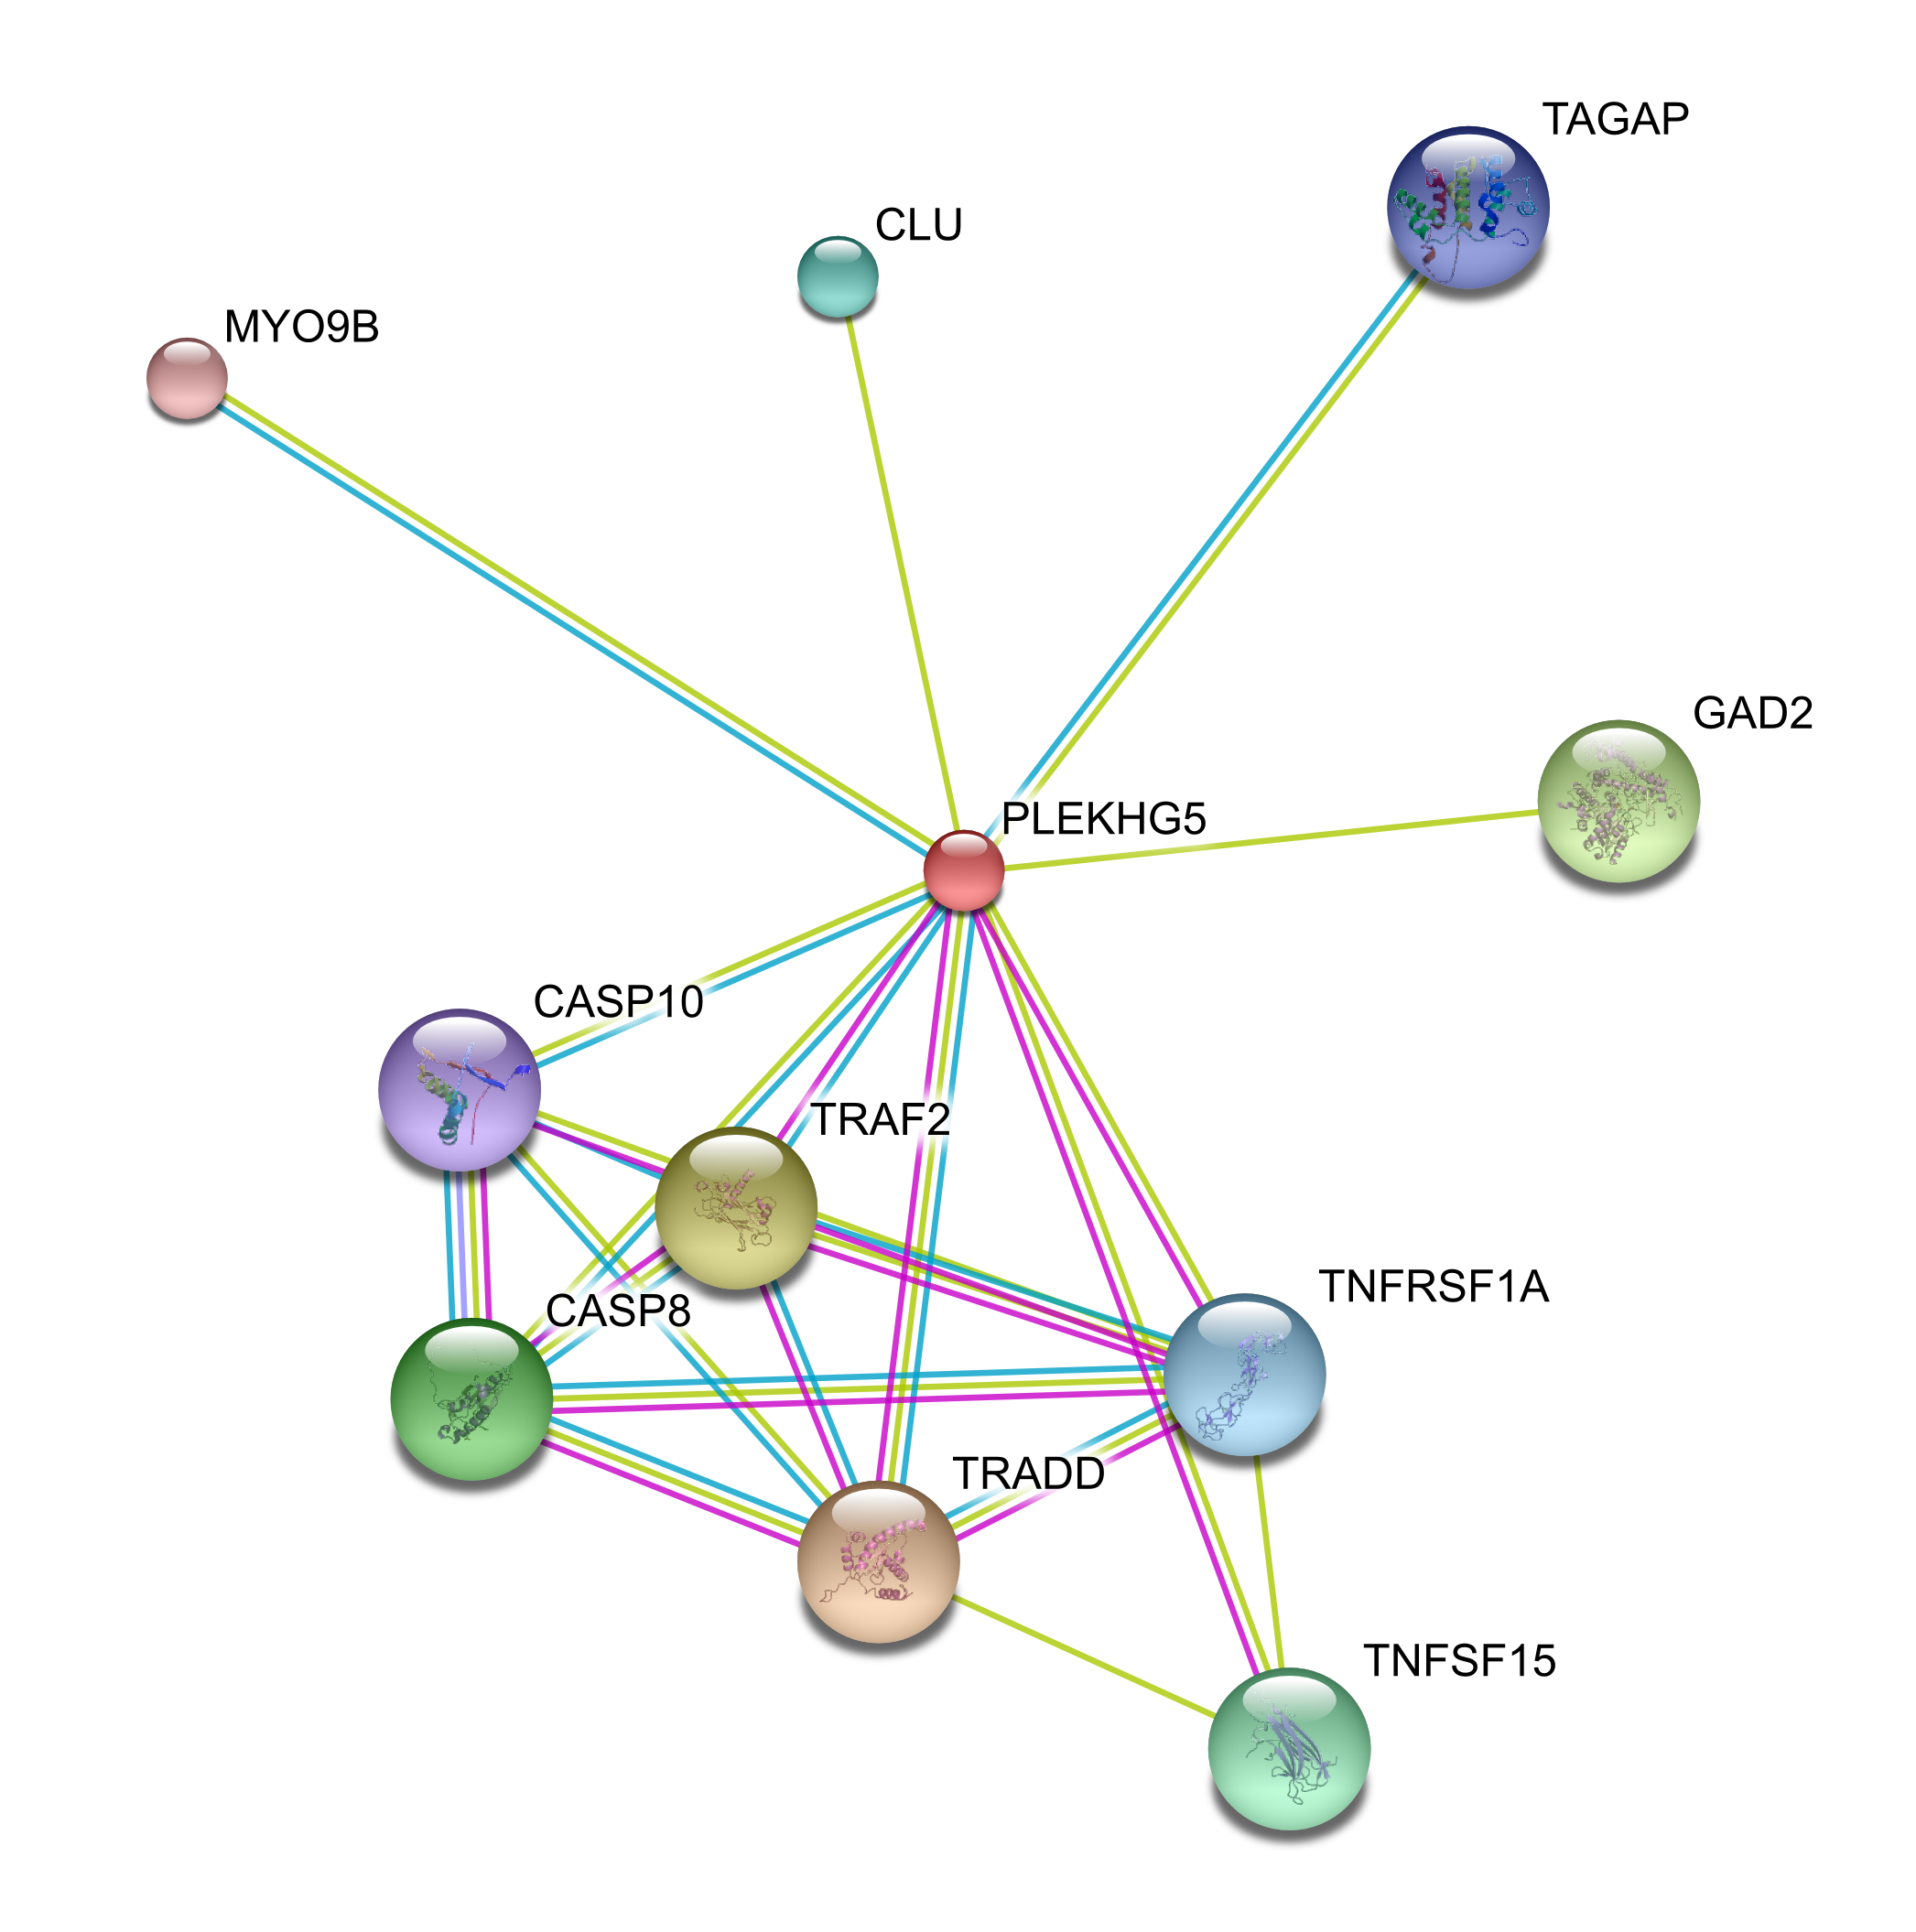
\includegraphics[scale=.7]{imgs/PLEKHG5}
	\caption{Rede de livre-escala}
	Fonte: \cite{Barabasi:a04}
	\label{fgr:RedeLivreEscala}
\end{figure}

A rela��o entre a topologia de uma rede biol�gica e suas propriedades funcionais e evolucion�rias sugerem a maioria das redes biol�gicas, s�o redes de livre-escala: redes de sinaliza��o, redes celulares, redes metab�licas e redes de intera��o de prote�nas \cite{Siegal:a07}.

\subsection{Redes de sinaliza��o}

Redes de sinaliza��o (\emph{signaling networks}) s�o complexas em termos de eventos qu�micos e biof�sicos e um grande n�mero de intera��es. A descri��o quantitativa nos modelos facilita o mapeamento entre diferentes tipos de m�todos de an�lise para sistemas complexos. M�todos de analise de sistemas podem ressaltar estados est�veis da rede de sinaliza��o e descrever as transi��es entre eles. Modelos tamb�m revelam funcionalidades similares entre propriedades das redes de sinaliza��o e outros sistemas bem-compreendidos, tais como, dispositivos eletr�nicos e redes neurais \cite{Bhalla:a03}.

\pagebreak

� poss�vel considerar redes de sinaliza��o como sistemas que decodificam entradas complexas em tempo, espa�o e qu�mica em padr�es combinat�rios de sa�da de atividades de sinaliza��o. A combina��o de m�todos de modelos de computa��o para capturar a complexidade e detalhes, e abstra��es �teis reveladas por estes modelos, � necess�rio para alcan�ar uma descri��o rigorosa t�o boa quanto � compreens�o humana \cite{Bhalla:a03}.

\subsection{Redes celulares}

As redes celulares (\emph{cellular networks}) s�o redes de livre-escala. A primeira evid�ncia desta afirma��o surgiu da an�lise do metabolismo, no qual os nodos s�o o resultado da atividade metab�lica e as liga��es representam rea��es bioqu�micas de catalise enzim�tica. Assim como as rea��es s�o irrevers�veis, redes metab�licas s�o direcionadas \cite{Barabasi:a04}.

\subsection{Redes metab�licas}

Uma rede metab�lica (\emph{metabolic networks}) � uma rede de caminhos aonde substratos e produtos metab�licos s�o conectados com arestas dirigidas. Estes arcos indicam atos de rea��es metab�licas sobre um determinado substrato e produz um determinado produto. Estudar redes metab�licas permite compreender os mecanismos moleculares de um organismo espec�fico, como por exemplo, glic�lise, ciclo de Krebs, etc \cite{Bebek:a07}.

\subsection{Redes de intera��o de prote�nas}

A topologia de livre-escala � tamb�m, aparentemente, uma caracter�stica das redes de intera��o de prote�nas (\emph{protein-protein interaction network}), embora as limita��es nos dados sejam substanciais. Redes de intera��o de prote�nas s�o determinadas, primeiramente, pela an�lise de duas leveduras h�bridas, as quais n�o provam intera��es nativas \cite{Siegal:a07}.

As ontologias servem para classificar as redes conforme suas fun��es biol�gicas, que podem ser componente celular, processo biol�gico e fun��o molecular.

\section{Ontologia g�nica}

O projeto Ontologia G�nica\footnote{The Gene Ontology Project. Dispon�vel em: $<$\url{http://www.geneontology.org}$>$. Acesso em: 24 de abril de 2009} (\emph{Gene Ontology} ou GO) � uma das principais iniciativas na bioinform�tica e tamb�m um esfor�o de colabora��o para dar resposta � necessidade de coer�ncia na descri��o dos produtos de gene em diferentes bases de dados. O projeto tamb�m � parte de um esfor�o maior para classifica��o, o \emph{Open Biomedical Ontologies} (OBO) \cite{Ferro:m08}.

Existem tr�s aspectos distintos para este esfor�o: em primeiro lugar, escrever e manter as ontologias (vocabul�rio controlado de gene e propriedades produto de gene) em si, em segundo lugar, fazer liga��es cruzadas entre as ontologias e os genes e produtos de gene buscando difundir e assimilar as anota��es de dados; e em terceiro lugar, desenvolver ferramentas que facilitam a cria��o, manuten��o e uso de ontologias. Atualmente o projeto GO est� organizado em tr�s princ�pios: componente celular, que � um componente de uma c�lula, mas com a ressalva de que � parte de um objeto maior que pode ser uma estrutura anat�mica; processo biol�gico, que � uma s�rie de eventos que � realizada por um ou mais conjuntos de fun��es moleculares ordenadas; e fun��o molecular, que descreve atividades, tais como catalisadores, por exemplo, que ocorrem ao n�vel molecular. Esses tr�s princ�pios ou �reas s�o considerados independentes umas das outras \cite{Ferro:m08}.

O projeto GO foi originalmente constitu�do em 1998 por um cons�rcio de investigadores dedicados a estudar o genoma de tr�s organismos modelo: \emph{Drosophila melanogaster} (mosca das frutas), \emph{Mus musculus} (rato), e \emph{Saccharomyces cerevisiae} (levedura). Muitas outras bases de organismo modelo aderiram ao projeto formando o cons�rcio GO (\emph{GO Consortium}), que � o conjunto de grupos envolvidos ativamente no projeto GO, contribuindo n�o s� com anota��o de dados, mas tamb�m para o desenvolvimento de ontologias e ferramentas para visualizar e aplicar os dados.

\pagebreak

Em janeiro de 2008, o projeto GO j� continha mais de 24.500 termos aplic�veis a uma ampla variedade de organismos biol�gicos. Atualmente existe um conjunto significativo de literatura sobre o desenvolvimento e a utiliza��o do projeto GO e o mesmo j� se tornou uma ferramenta padr�o no arsenal da bioinform�tica.

\section{Fluxo de pesquisa de uma doen�a}

O fluxo de pesquisa para gera��o das redes de intera��o da prote�na pode seguir dois fluxos, para tanto os mesmos ser�o descritos separadamente nas se��es seguintes usando como base a Figura \ref{fgr:FluxoPesquisa}.

\begin{figure}[htp]
	\centering
	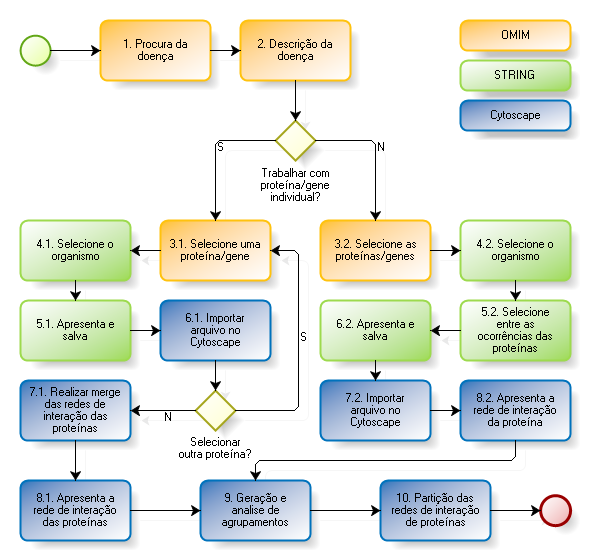
\includegraphics[scale=.65]{imgs/FluxoPesquisa2}
	\caption{Fluxo de pesquisa}
	\label{fgr:FluxoPesquisa}
\end{figure}

\subsection{Descri��o do Fluxo A}
\label{sbsct:DescricaoFluxoA}

O Fluxo A de pesquisa ocorre da seguinte forma. Primeiramente acesse o \emph{site} do OMIM, em \url{http://www.ncbi.nlm.nih.gov/omim}, digite na caixa de texto ao lado do \emph{label} ``for'' a doen�a que procura, como mostra a Figura \ref{fgr:Etapa01}, e depois clique no bot�o ``Go'' (Atividade 1).

\begin{figure}[htp]
	\centering
	\framebox{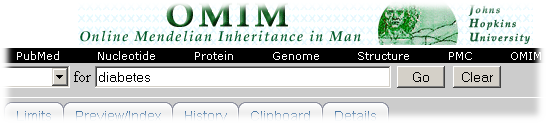
\includegraphics[width=.9\textwidth]{imgs/Etapa01}}
	\caption{Pesquisa da doen�a}
	\label{fgr:Etapa01}
\end{figure}

Ent�o o \emph{site} lhe apresentar� uma lista com as ocorr�ncias da doen�a para que voc� selecione a que voc� est� procurando, como mostra a Figura \ref{fgr:Etapa02}.

\begin{figure}[htp]
	\centering
	\framebox{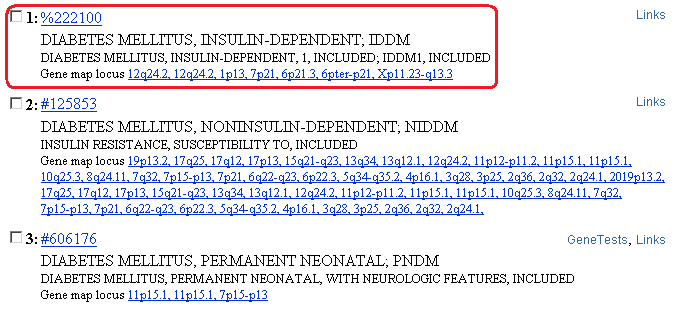
\includegraphics[width=.9\textwidth]{imgs/Etapa02}}
	\caption{Lista de ocorr�ncias da doen�a}
	\label{fgr:Etapa02}
\end{figure}

Ap�s escolhida a ocorr�ncia da doen�a, o \emph{site} lhe apresentar� um relat�rio com a descri��o completa da mesma, como mostra a Figura \ref{fgr:Etapa03} (Atividade 2).

\begin{figure}[htp]
	\centering
	\framebox{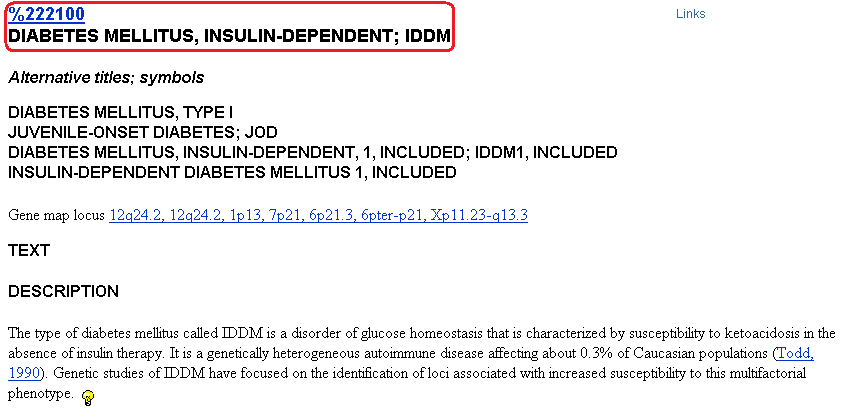
\includegraphics[width=.9\textwidth]{imgs/Etapa03}}
	\caption{Relat�rio da doen�a}
	\label{fgr:Etapa03}
\end{figure}

Ent�o localize e selecione uma ou mais prote�nas/genes (no exemplo, sublinhadas em vermelho) no relat�rio, como mostra a Figura \ref{fgr:Etapa04} (Atividade 3.1).

\begin{figure}[htp]
	\centering
	\framebox{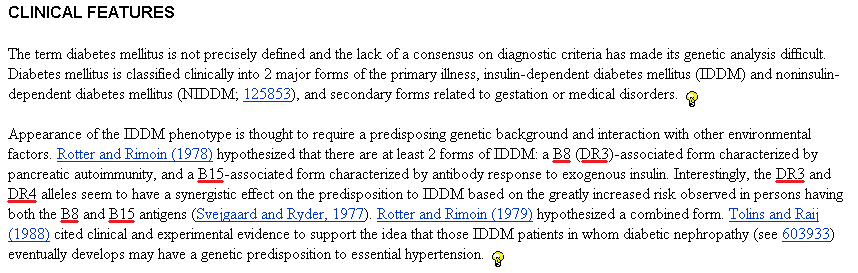
\includegraphics[width=.9\textwidth]{imgs/Etapa04}}
	\caption{Localizando prote�nas/genes no relat�rio}
	\label{fgr:Etapa04}
\end{figure}

Ap�s selecionada a prote�na, acesse o \emph{site} do STRING, em \url{http://string.embl.de}, e digite-a na caixa de texto localizada abaixo do \emph{label} ``protein name:'' na aba ``search by name'', como mostra a Figura \ref{fgr:Etapa05-1} e clique no bot�o ``GO !''.

\begin{figure}[htp]
	\centering
	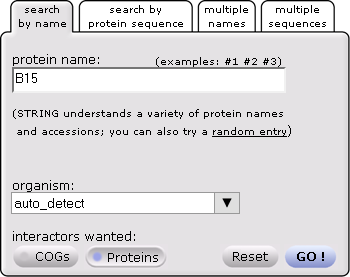
\includegraphics[scale=.9]{imgs/Etapa05-1}
	\caption{Pesquisa da prote�na}
	\label{fgr:Etapa05-1}
\end{figure}

O \emph{site} lhe apresentar� uma lista de organismos, como mostra a Figura \ref{fgr:Etapa06-1}, selecione o que deseja utilizar e clique no bot�o ``Continue $\rightarrow$'' para prosseguir para a pr�xima etapa (Atividade 4.1).

\begin{figure}[htp]
	\centering
	\framebox{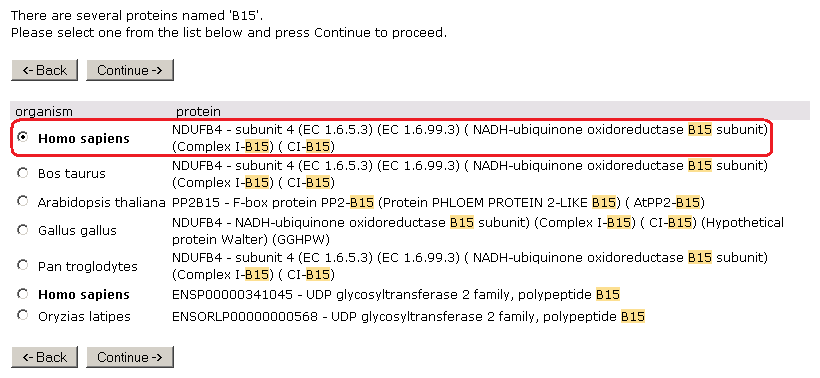
\includegraphics[width=.9\textwidth]{imgs/Etapa06-1}}
	\caption{Lista de organismos que possuem a prote�na}
	\label{fgr:Etapa06-1}
\end{figure}

Ent�o lhe ser� apresentada a rede de intera��o da prote�na, como mostra a Figura \ref{fgr:Etapa07-1}, clique no bot�o ``save'' para prosseguir (Atividade 5.1).

\begin{figure}[htp]
	\centering
	\framebox{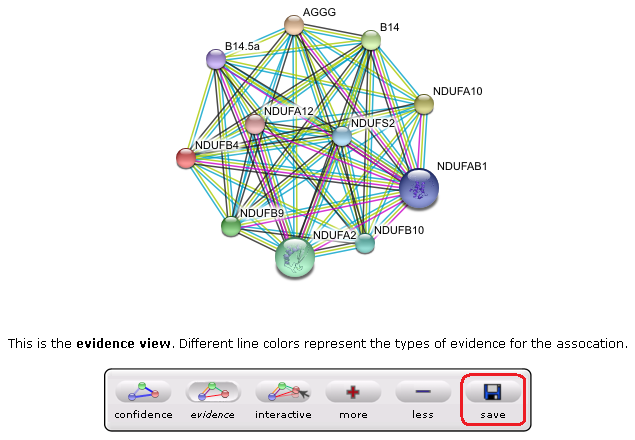
\includegraphics[width=.9\textwidth]{imgs/Etapa07-1}}
	\caption{Apresenta��o da rede de intera��o da prote�na}
	\label{fgr:Etapa07-1}
\end{figure}

Ap�s isso o \emph{site} lhe apresentar� uma �ltima tela solicitando que voc� escolha o tipo de arquivo que deseja salvar, como mostra a Figura \ref{fgr:Etapa08-1}, selecione o arquivo do tipo XML (no exemplo, circulado em vermelho).

\begin{figure}[htp]
	\centering
	\framebox{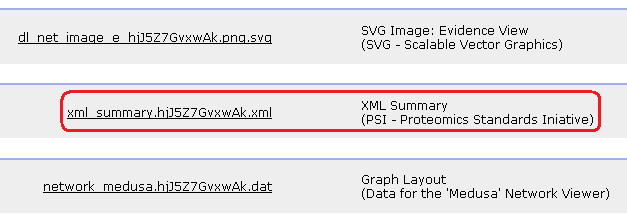
\includegraphics[width=.9\textwidth]{imgs/Etapa08-1}}
	\caption{Sele��o do tipo de arquivo da rede de intera��o}
	\label{fgr:Etapa08-1}
\end{figure}

\pagebreak

Uma vez que o arquivo esteja salvo em sua m�quina local, abra o software ``Cytoscape'', dispon�vel em \url{http://www.cytoscape.org}, e abra o menu ``File $\rightarrow$ Import $\rightarrow$ Network (multiple file types)\dots'' (Atividade 6.1).

Selecione o arquivo que deseja importar clicando no bot�o ``Select'' e o localizando, ent�o clique no bot�o ``Import'' para importar o arquivo, como mostra a Figura \ref{fgr:Etapa09-1}. Repita esse processo com quantas prote�nas voc� desejar.

\begin{figure}[htp]
	\centering
	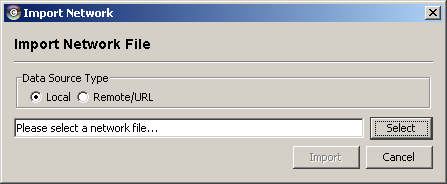
\includegraphics[width=.9\textwidth]{imgs/Etapa09-1}
	\caption{Importando rede de intera��o da(s) prote�na(s)}
	\label{fgr:Etapa09-1}
\end{figure}

Uma vez que todos os arquivos que deseja utilizar tenham sido importados, voc� poder� realizar um ``merge'' das redes de intera��es. Abra o menu ``Plugins $\rightarrow$ Merge networks'', selecione as redes que deseja realizar o ``merge'', como mostra a Figura \ref{fgr:Etapa10-1}, e clique em ``OK'' (Atividade 7.1).

\begin{figure}[htp]
	\centering
	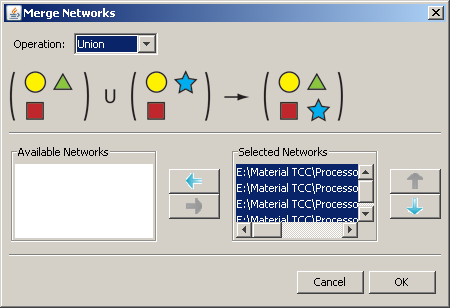
\includegraphics[width=.9\textwidth]{imgs/Etapa10-1}
	\caption{Merge das redes de intera��es das prote�nas}
	\label{fgr:Etapa10-1}
\end{figure}

Ap�s isso voc� ter� a representa��o gr�fica do ``merge'' das redes de intera��es, como mostra a Figura \ref{fgr:Etapa11-1} (Atividade 8.1).

\begin{figure}[ht]
	\centering
	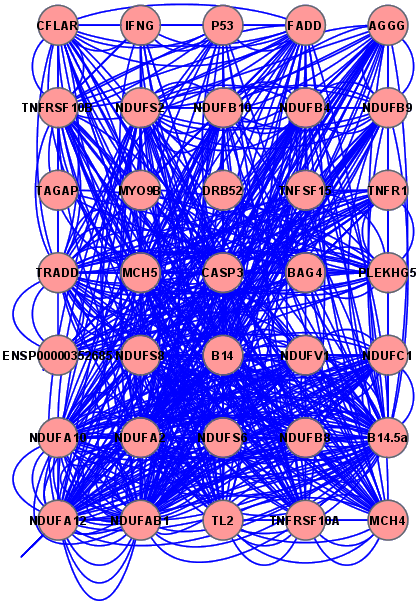
\includegraphics[scale=.6]{imgs/Etapa11-1}
	\caption{Representa��o gr�fica das redes de intera��es}
	\label{fgr:Etapa11-1}
\end{figure}

Uma vez que o especialista tenha essa rede de intera��es, ele pode fazer a an�lise dos agrupamentos dessa rede atrav�s do \emph{plug-in} dispon�vel para o software Cytoscape chamado ``MCODE''. O MCODE\footnote{MCODE. Dispon�vel em: $<$\url{http://chianti.ucsd.edu/cyto_web/plugins/index.php}$>$. Acesso em: 17 de junho de 2009} � respons�vel por encontrar \emph{clusters} (regi�es altamente conectadas) em uma rede, pois aglomerados significam coisas diferentes em tipos de redes diferentes (Atividade 9).

Ent�o o especialista pode fazer a parti��o das redes de intera��o de prote�nas usando a ontologia g�nica atrav�s de outro \emph{plug-in} dispon�vel para o software Cytoscape chamado ``BiNGO''. O BiNGO\footnote{BiNGO. Dispon�vel em: $<$\url{http://www.psb.ugent.be/cbd/papers/BiNGO}$>$. Acesso em: 17 de junho de 2009} � respons�vel por determinar quais as categorias de ontologia g�nica est�o estatisticamente sendo representadas em um conjunto de genes ou o sub gr�fico biol�gico de uma rede (Atividade 10).

\subsection{Descri��o do Fluxo B}

O Fluxo B de pesquisa ocorre da seguinte forma. Primeiramente acesse o \emph{site} do OMIM, em \url{http://www.ncbi.nlm.nih.gov/omim}, e digite na caixa de texto ao lado do \emph{label} ``for'' a doen�a que procura, como mostra a Figura \ref{fgr:Etapa01} apresentada na Subse��o \ref{sbsct:DescricaoFluxoA}, e depois clique no bot�o ``Go'' (Atividade 1).

Ent�o o \emph{site} lhe apresentar� uma lista com as ocorr�ncias da doen�a para que voc� selecione a que voc� est� procurando, como mostra a Figura \ref{fgr:Etapa02} apresentada na Subse��o \ref{sbsct:DescricaoFluxoA}.

Ap�s escolhida a ocorr�ncia da doen�a, o \emph{site} lhe apresentar� um relat�rio com a descri��o completa da mesma, como mostra a Figura \ref{fgr:Etapa03} apresentada na Subse��o \ref{sbsct:DescricaoFluxoA} (Atividade 2).

Ent�o localize e selecione uma ou mais prote�nas/genes (no exemplo, sublinhadas em vermelho) no relat�rio, como mostra a Figura \ref{fgr:Etapa04} apresentada na Subse��o \ref{sbsct:DescricaoFluxoA} (Atividade 3).

Acesse o \emph{site} do STRING, em \url{http://string.embl.de}, e digite na caixa de texto localizada abaixo do \emph{label} ``list of names:'' na aba ``multiple names'', cada uma das prote�nas selecionadas que deseja utilizar, como mostra a Figura \ref{fgr:Etapa05-2} e clique no bot�o ``GO !''.

\begin{figure}[htp]
	\centering
	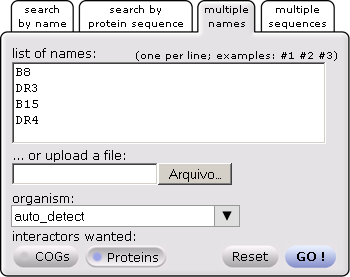
\includegraphics[scale=.9]{imgs/Etapa05-2}
	\caption{Pesquisa das prote�nas}
	\label{fgr:Etapa05-2}
\end{figure}

O \emph{site} lhe apresentar� uma lista de organismos, como mostra a Figura \ref{fgr:Etapa06-2}, selecione o que deseja utilizar e clique no bot�o ``Continue $\rightarrow$'' para prosseguir para a pr�xima etapa (Atividade 4.2).

\begin{figure}[htp]
	\centering
	\framebox{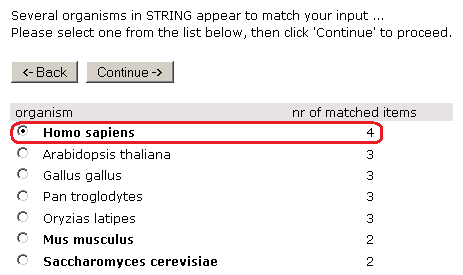
\includegraphics[width=.9\textwidth]{imgs/Etapa06-2}}
	\caption{Lista de organismos que possuem as prote�nas}
	\label{fgr:Etapa06-2}
\end{figure}

\pagebreak

Ent�o o \emph{site} lhe apresentar� uma nova lista pendido que voc� selecione dentre as ocorr�ncias das prote�nas quais ser�o utilizadas, como mostra a Figura \ref{fgr:Etapa07-2}, selecione-as e clique no bot�o ``Continue $\rightarrow$'' novamente. Pode-se ressaltar que combina��es diferentes geram redes diferentes (Atividade 5.2).

\begin{figure}[htp]
	\centering
	\framebox{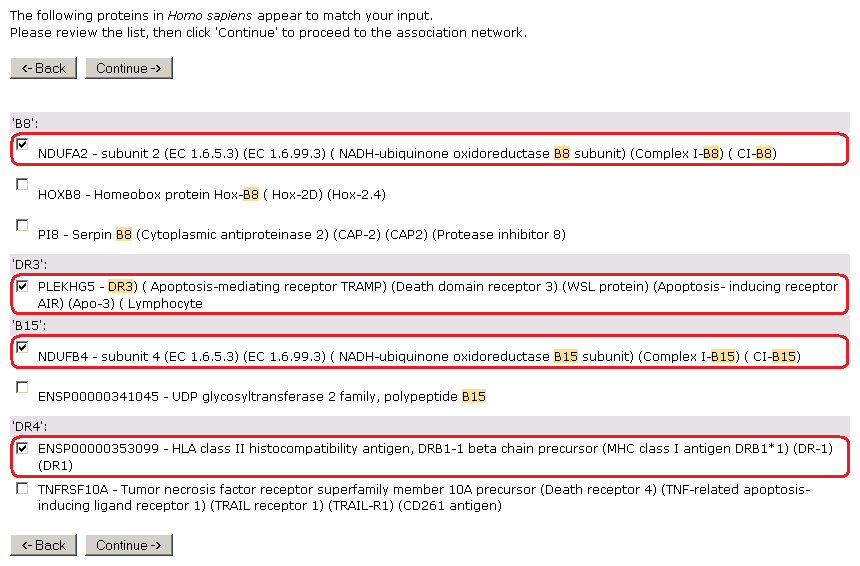
\includegraphics[width=.9\textwidth]{imgs/Etapa07-2}}
	\caption{Lista de ocorr�ncias das prote�nas}
	\label{fgr:Etapa07-2}
\end{figure}

Ent�o lhe ser� apresentada a rede de intera��o das prote�nas, como mostra a Figura \ref{fgr:Etapa08-2}, clique no bot�o ``save'' para prosseguir (Atividade 6.2).

\begin{figure}[htp]
	\centering
	\framebox{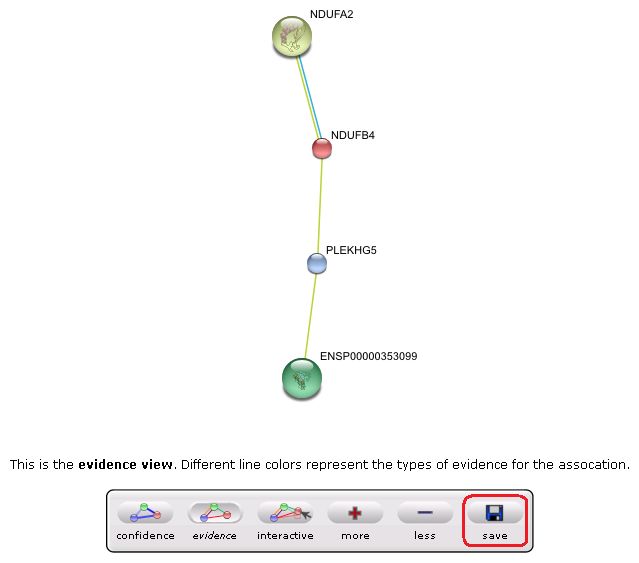
\includegraphics[width=.9\textwidth]{imgs/Etapa08-2}}
	\caption{Apresenta��o da rede de intera��o das prote�nas}
	\label{fgr:Etapa08-2}
\end{figure}

Ap�s isso o \emph{site} lhe apresentar� uma �ltima tela solicitando que voc� escolha o tipo de arquivo que deseja salvar, como mostra a Figura \ref{fgr:Etapa09-2}, selecione o arquivo do tipo XML (no exemplo, circulado em vermelho).

\begin{figure}[htp]
	\centering
	\framebox{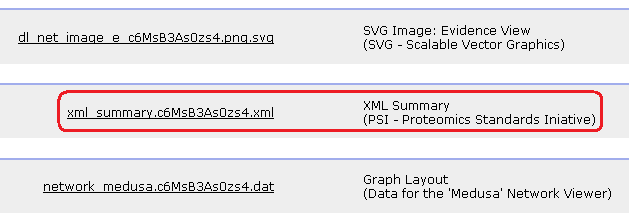
\includegraphics[width=.9\textwidth]{imgs/Etapa09-2}}
	\caption{Sele��o do tipo de arquivo das redes de intera��es}
	\label{fgr:Etapa09-2}
\end{figure}

Uma vez que o arquivo esteja salvo em sua m�quina local, abra o software ``Cytoscape'', dispon�vel em \url{http://www.cytoscape.org}, e abra o menu ``File $\rightarrow$ Import $\rightarrow$ Network (multiple file types)\dots'' (Atividade 7.2).

Selecione o arquivo que deseja importar clicando no bot�o ``Select'' e o localizando, ent�o clique no bot�o ``Import'' para importar o arquivo, como mostra a Figura \ref{fgr:Etapa09-1} apresentada na Subse��o \ref{sbsct:DescricaoFluxoA}.

Ap�s isso voc� ter� a representa��o gr�fica da rede de intera��o, como mostra a Figura \ref{fgr:Etapa10-2} (Atividade 8.2).

\begin{figure}[ht]
	\centering
	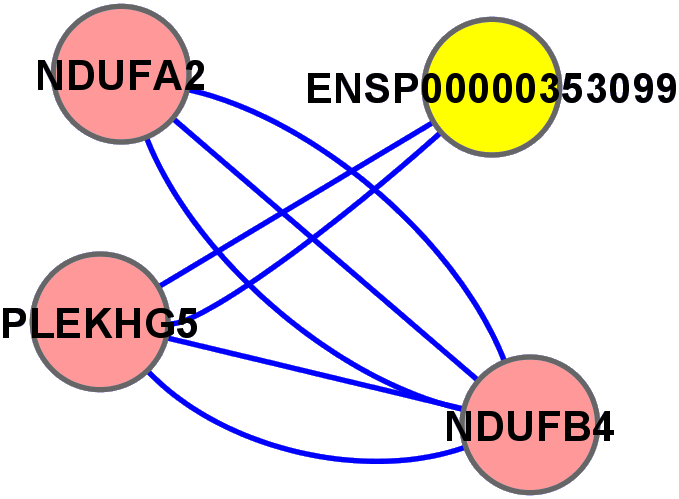
\includegraphics[scale=.4]{imgs/Etapa10-2}
	\caption{Representa��o gr�fica das redes de intera��es}
	\label{fgr:Etapa10-2}
\end{figure}

Uma vez que o especialista tenha essa rede de intera��es, ele pode fazer a an�lise dos agrupamentos dessa rede atrav�s do \emph{plug-in} dispon�vel para o software Cytoscape chamado ``MCODE'' (Atividade 9).

Ent�o o especialista pode fazer a parti��o das redes de intera��o de prote�nas usando a ontologia g�nica atrav�s de outro \emph{plug-in} dispon�vel para o software Cytoscape chamado ``BiNGO'' (Atividade 10).

\section{Considera��es finais}

Nesse cap�tulo foi apresentado o fluxo de pesquisa de uma doen�a g�nica que ser� trabalhado nos pr�ximos cap�tulos, explicando os conceitos necess�rios ao seu entendimento.

Para levantamento dos requisitos do sistema foi necess�ria uma reuni�o presencial com o especialista, nessa reuni�o foi explicado o fluxo de pesquisa de uma doen�a g�nica, bem como os \emph{sites} utilizados. Tamb�m foi levantada a forma que o fluxo era documentado para, posteriormente, repetir o experimento e descobriu-se que � feito de forma manual.

Ent�o foram acessados os \emph{sites} do OMIM e do STRING, pelo especialista, e foi mostrado passo-a-passo como eram feitas as buscas por doen�as g�nicas, por genes/prote�nas no relat�rio da doen�a e, posteriormente, pelas redes de intera��o de prote�nas. Outras d�vidas que surgiram durante a documenta��o do fluxo foram esclarecidas por \emph{e-mail} com o especialista.

\pagebreak

Feito isso, o fluxo de pesquisa de uma doen�a g�nica foi documentado com a cria��o de um \emph{workflow}, o qual demonstra os passos realizados pelo especialista. Esse \emph{workflow} teve todos os seus passos descritos e explicados com o aux�lio de imagens retiradas dos \emph{sites}.

No pr�ximo cap�tulo ser� apresentada a proposta de software para facilitar e tornar mais confi�vel esse fluxo de pesquisa.
	\chapter{Proposta de software}
\label{cap:PropostaSoftware}

Neste cap�tulo ser�o apresentadas algumas ferramentas para o desenvolvimento de \emph{workflows} cient�ficos, as regras de nomenclatura gen�tica e a modelagem do software a ser desenvolvido para utilizar a biologia de sistemas, para an�lise de uma rede de intera��o de prote�nas a partir da pesquisa sobre doen�as gen�ticas.

\section{Workflow}

Um \emph{workflow} � uma seq��ncia de atividades ao longo de um processo de neg�cio, completo ou apenas parte dele, onde documentos, informa��es ou tarefas s�o transmitidas de um participante a outro por a��es, de acordo com regras procedimentais \cite{Mattos:m08, Sommerville:l07}.

\emph{Workflows} cient�ficos s�o definidos como recursos para resolu��o de problemas cient�ficos atrav�s de t�cnicas tradicionais de \emph{workflows}, ou seja, as id�ias de execu��o de um conjunto de tarefas em uma determinada seq��ncia foram aproveitadas na �rea cient�fica para a realiza��o de experimentos e estudos. \emph{Workflows} cient�ficos diferem de \emph{workflows} de neg�cio em diversos aspectos, particularmente em bioinform�tica, s�o caracterizados pelo alto grau de interven��o humana durante a sua execu��o \cite{Digiampietri:m07, Silva:m06}. Nas subse��es que seguem, ser�o apresentadas algumas ferramentas para o desenvolvimento de \emph{workflows} cient�ficos.

\subsection{VisTrails}

O VisTrails\footnote{VisTrails. Dispon�vel em: $<$\url{http://www.vistrails.org}$>$. Acesso em: 10 de junho de 2009} foi concebido para gerenciar a r�pida evolu��o dos \emph{workflows}. VisTrails simplifica a cria��o, execu��o e compartilhamento de visualiza��es complexas, minera��es de dados ou outos dados de an�lise em larga escala. Ao gerir automaticamente os dados, metadados, e os dados de explora��o de processos, VisTrails permite que os usu�rios se concentrem em tarefas complexas e desafiadoras e os libera de tarefas tediosas que comsomem muito tempo, como as relacionadas a organiza��o e manipula��o de grandes volumes de dados.

VisTrails fornece uma infra-estrutura que pode ser combinada com a de sistemas de visualiza��o e de \emph{workflow} existentes. Embora o VisTrails tenha sido originalmente constru�do para atender as necessidades de aplica��es cient�ficas explorat�rias, a infra-estrutura que oferece � muito geral. Isto tornou claro que o sistema foi desenvolvido para pessoas de diferentes dom�nios, tanto para ind�strias como para universidades. VisTrails tem potencial para reduzir o tempo de introspec��o em praticamente qualquer tarefa explorat�ria.

\subsection{Kepler}

Kepler\footnote{Kepler. Dispon�vel em: $<$\url{https://kepler-project.org}$>$. Acesso em: 10 de junho de 2009} foi concebido para ajudar os cientistas, os analistas e os programadores a criar, executar e compartilhar modelos e an�lises sobre uma vasta gama de disciplinas cient�ficas e de engenharia. Kepler pode operar sobre os dados armazenados em uma variedade de formatos, locais e atrav�s da Internet, e � um meio eficaz para a integra��o de d�spares componentes de software, ou facilitar a distribui��o e execu��o de modelos remotos. Usando a interface gr�fica do usu�rio, basta selecionar os usu�rios e em seguida, conectar componentes anal�ticos pertinentes e fontes de dados para criar um ``trabalho cient�fico'' (representa��o de passos necess�rios para gerar resultados). O software Kepler ajuda os usu�rios a compartilhar e reutilizar dados, fluxos de trabalho e componentes desenvolvidos pela comunidade cient�fica para resolver necessidades comuns.

O software Kepler � desenvolvido e mantido pelo \emph{the cross-project Kepler collaboration}, que � liderado por uma equipe constitu�da por v�rios das principais institui��es que originaram o projeto: UC Davis, UC Santa Barbara e UC San Diego. Primeiramente respons�vel pela concretiza��o dos objetivos do Projeto Kepler a longo prazo, essa equipe trabalha para garantir a viabilidade t�cnica e financeira do Kepler, tomando as decis�es estrat�gicas em nome da comunidade de usu�rios do Kepler, bem como proporcionar um ponto de contato oficial e duradouro para representar os interesses do Projeto Kepler.

Kepler � uma aplica��o baseada em Java e � matido os sistemas operaconais Windows, OSX e Linux. O Projeto Kepler ap�ia o desenvolvimento do Kepler como c�digo aberto, bem como fornece materiais e mecanismos para aprendizagem de como usar o Kepler, o compartilhamento de experi�ncias com outros desenvolvedores de \emph{workflow}, relatando \emph{bugs}, sugerindo melhorias, etc.

\subsection{Taverna}

O Taverna Workbench\footnote{Taverna Workbench. Dispon�vel em: $<$\url{http://taverna.sourceforge.net}$>$. Acesso em: 10 de junho de 2009} � uma ferramenta de software livre para projetar e executar os fluxos de trabalho, criada pelo Projeto myGrid e financiada pelo OMII-UK.

Taverna permite que os usu�rios integrem diversas ferramentas, incluindo os \emph{web services} de diferentes dom�nios, como a qu�mica, a m�sica e as ci�ncias sociais. Para bionform�tica fornece acesso aos \emph{services} prestados pela \emph{National Center for Biotechnology Information, The European Bioinformatics Institute, the DNA Databank of Japan (DDBJ), SoapLab, BioMOBY} e \emph{EMBOSS}.

O Taverna Workbench fornece um ambiente desktop para cria��o de \emph{workflow} cient�ficos. O \emph{myExperiment social site} suporta procura e partilha de fluxos de trabalho e tem um suporte especial para Taverna \emph{workflow}. O Taverna workbench, myExperiment e respectivos componentes s�o desenvolvidos e mantidos pela equipe do myGrid em colabora��o com a comunidade de fonte aberta.

O Taverna roda em qualquer vers�o Windows, Linux, OSX e outros sistemas UNIX recentes. Se o seu computador tem uma conex�o de rede e consegue executar o Java 5, voc� n�o precisa de mais nada, pois n�o existem bases de dados e nem an�lise de instalar aplica��es, j� que todos estes s�o acessados atrav�s da rede.

\subsection{Egene}

O Egene\footnote{Egene. Dispon�vel em: $<$\url{http://www.coccidia.icb.usp.br/egene}$>$. Acesso em: 10 de junho de 2009} � um sistema gen�rico, flex�vel e modular para constru��o de \emph{workflow} de trabalho, permite que programas de terceiros sejam utilizados e integrados segundo as necessidades de diferentes projetos e sem qualquer programa��o ou experi�ncia a ser exigida.

O Egene vem com Coed, uma ferramenta visual que facilita a constru��o e documenta��o. Egene � um software de c�digo aberto e foi desenvolvido para rodar em sistemas operacionais Unix/Linux. O sistema Egene foi escrito em Perl.

\section{Nomenclatura gen�tica}

As regras de nomenclatura gen�tica aprovadas pelo \emph{HUGO Gene Nomenclature Committee} (HGNC) informam que, os nomes dos genes devem ser breves, espec�ficos e devem tentar trazer informa��es sobre sua fun��o e rela��o com os outros genes da mesma fam�lia \cite{Wain:09, Wain:a04, Wain:a02}.

Tamb�m informam que, a primeira letra do nome do gene deve ser a mesma do s�mbolo do gene, para facilitar a localiza��o, os nomes dos genes devem ser descritos na ortografia americana, a especificidade dos tecidos e o peso molecular devem ser evitados, podendo estes ser usados de forma ilimitada na descri��o, e os nomes n�o devem usar termos para definir rela��es familiares com outros genes \cite{Splendore:a05, Wain:09, Wain:a04, Wain:a02-2}. Segundo \cite{HGNC:09, Wain:09, Wain:a04, Wain:a02}, os nomes de genes devem seguir as seguintes regras:

\begin{itemize}
	\item Come�am com letra min�scula, a n�o ser que seja o nome de uma pessoa que descreva a doen�a;
	\item Modificadores descritivos devem seguir a parte principal do nome, separados por v�rgulas;
	\item Caso exista um nome alternativo esse deve ser colocado entre par�nteses; e
	\item Caso exista um nome de outras esp�cies esse deve ser colocado entre parentes e no final do nome.
\end{itemize}

Os genes, al�m do nome oficial, tamb�m possuem um s�mbolo usado para design�-los em bancos de dados e publica��es. Os s�mbolos dos genes s�o caracterizados por letras mai�sculas ou uma combina��o de letras mai�sculas e algarismos ar�bicos, com exce��o dos s�mbolos C\#orf\# \cite{Wain:09, Wain:a04, Wain:a02}. Segundo \cite{Eyre:a06, Fundel:a06}, os s�mbolos de genes devem seguir as seguintes regras:

\begin{itemize}
	\item Devem ser curtos, preferencialmente com menos de seis caracteres de comprimento;
	\item Devem iniciar com uma letra mai�scula e podem ser seguidos de outras letras mai�sculas ou algarismos ar�bicos;
	\item N�o podem conter sobre ou subscritos, algarismos romanos, letras gregas, pontua��o (com exce��o do gene HLA), ``G'' para a identifica��o de gene, ou qualquer outra refer�ncia a esp�cie, por exemplo, ``H / h'' para humanos;
	\item Devem ser evitadas refer�ncias a especificidade dos tecidos, peso molecular e localiza��o cromoss�mica; e
	\item Tamb�m devem ser evitadas algumas letras ou combina��o de letras que s�o usadas como prefixo ou sufixo em um s�mbolo para dar um significado espec�fico, devendo essas n�o ser utilizadas para outros fins.
\end{itemize}

Embora existam in�meras exce��es, os genes e as prote�nas derivadas carregam o mesmo nome/s�mbolo sendo essa inclusive uma recomenda��o do HGNC. Quando o mesmo s�mbolo � usado para designar o gene e a prote�na, a maneira de diferenci�-los � pelo uso de it�lico (por exemplo, gene \emph{GATA1}, prote�na GATA-1) \cite{Splendore:a05, Fundel:a06}. Na Tabela \ref{tbl:RegrasGrafia} � apresentado um resumo das regras de grafia para os s�mbolos dos genes humanos em trabalhos cient�ficos.

\pagebreak

\begin{table}[htp]
	\centering
	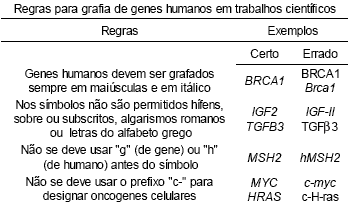
\includegraphics[scale=.9]{imgs/RegrasGrafia}
	\caption{Regras de Grafia}
	Fonte: \cite{Splendore:a05}
	\label{tbl:RegrasGrafia}
\end{table}

O benef�cio do uso de nomes e s�mbolos consistentes para os genes deve fazer com que um n�mero de revistas cada vez maior passe a exigir nas suas publica��es o cumprimento dessas regras, a exemplo do que j� fazem as principais revistas da �rea biom�dica, como a \emph{Nature, Nature Genetics, American Journal of Human Genetics, Genomics, Human Mulation, Genes Chromosomes Cancer} e \emph{The Lancet}. Para saber qual s�mbolo aprovado de um determinado gene, deve-se consultar a p�gina do HGNC/Genew, ou ent�o, procur�-lo no OMIM (\emph{Online Mendelian Inheritance in Man}) \cite{Splendore:a05, Fundel:a06}.

\section{Modelagem do software}

Nessa se��o ser�o apresentados os diagramas desenvolvidos com o objetivo de modelar o sistema \emph{web} e melhorar o entendimento quanto ao funcionamento do mesmo.

\subsection{Modelo de neg�cio - caso de uso}

O sistema tem o objetivo de facilitar o processo de an�lise das redes de intera��o prot�ica e possibilitar armazenar informa��es quanto � pesquisa durante o processo para posteriormente poderem ser usadas caso seja necess�rio reproduzir os passos da pesquisa, para isso o diagrama de caso de uso da Figura \ref{fgr:CasoDeUso01} visa demonstrar a intera��o dos usu�rios ``Bioinform�tica'' e ``Bi�logo'' com o ``Sistema Web'' e do ``Sistema Web'' com as outras aplica��es.

No caso de uso, os usu�rio interagem apenas com o ``Sistema Web'' e com o software de visualiza��o e an�lise da rede de intera��o de prote�nas, ficando os acessos a outras aplica��es, respons�veis pela pesquisa da doen�a e da prote�na, transparentes para o usu�rio.

\begin{figure}[htp]
	\centering
	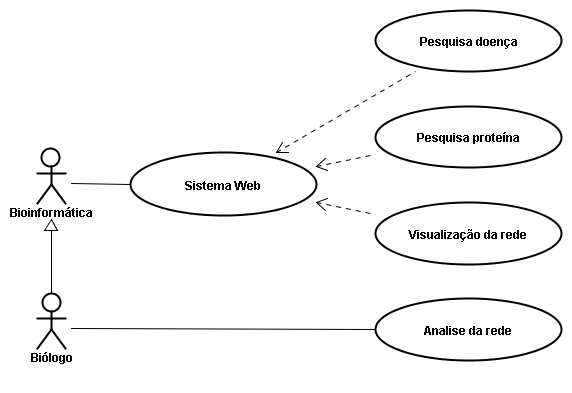
\includegraphics[scale=.55]{imgs/CasoDeUso01}
	\caption{Caso de Uso}
	\label{fgr:CasoDeUso01}
\end{figure}

\subsection{Workflow cient�fico para an�lise de redes de intera��o prot�ica}
\label{ssec:WorkflowCientifico}

O fluxo de pesquisa do software para gera��o da rede de intera��o da prote�na foi otimizado para prever interven��o humana e ser� explicado a seguir, usando como base a Figura \ref{fgr:FluxoPesquisaSoftware}.

\begin{figure}[htp]
	\centering
	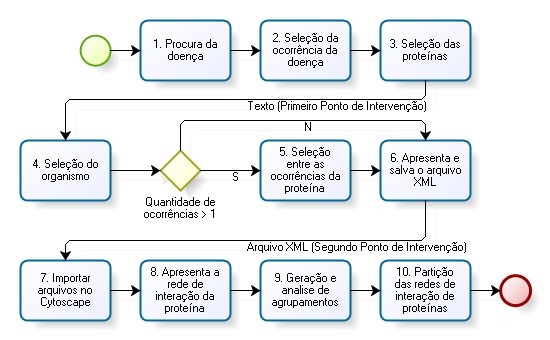
\includegraphics[scale=.75]{imgs/FluxoPesquisaSoftware2}
	\caption{Fluxo de pesquisa do software}
	\label{fgr:FluxoPesquisaSoftware}
\end{figure}

\pagebreak

O fluxo se inicia com o usu�rio digitando o nome da doen�a que deseja encontrar (Atividade 1), o acesso ao site do OMIM � feito atrav�s da busca passando par�metros pela url de chamada do site, por exemplo, \[ http://www.ncbi.nlm.nih.gov/sites/entrez?db=omim\&term=diabetes \] onde o par�metro ``db'' indica o banco de dados que est� sendo utilizado e ``term'' a doen�a que est� sendo procurada. Ent�o o sistema apresenta as ocorr�ncias encontradas para a doen�a e o usu�rio escolhe a que est� procurando (Atividade 2). Ap�s isso o sistema apresenta o relat�rio da doen�a e uma lista de sugest�es de prote�nas encontradas (Atividade 3). O sistema busca por essas prote�nas no site do STRING passando par�metros pela url de chamada do site, por exemplo, \[ http://string.embl.de/newstring\_cgi/show\_network\_section.pl?identifier=dr3 \] onde o par�metro ``identifier'' indica a prote�na que est� sendo procurada. Ent�o o sistema solicita que o usu�rio selecione o organismo que deseja utilizar (Atividade 4). Para o caso em que o site do STRING informar que foram encontradas mais de uma ocorr�ncia para o nome de uma prote�na, o sistema solicitar� que o usu�rio escolha dentre as ocorr�ncias quais ser�o utilizadas (Atividade 5). Ap�s isso o sistema apresentar� a rede de intera��o da(s) prote�na(s) e retornar� um arquivo XML (Atividade 6). Ent�o esse arquivo XML ser� importado no software Cytoscape (Atividade 7) e ser� apresentada a representa��o gr�fica da rede de intera��o da(s) prote�na(s) (Atividade 8).

Uma vez que o especialista tenha essa rede de intera��es, ele pode fazer a an�lise dos agrupamentos dessa rede atrav�s do \emph{plug-in} dispon�vel para o software Cytoscape chamado ``MCODE'' (Atividade 9). Ent�o o especialista pode fazer a parti��o das redes de intera��o de prote�nas usando a ontologia g�nica atrav�s de outro \emph{plug-in} dispon�vel para o software Cytoscape chamado ``BiNGO'' (Atividade 10).

\subsection{Diagrama de arquitetura da aplica��o}
\label{ssec:ArquiteturaAplicacao}

A arquitetura do sistema � enxuta, nela � necess�ria uma m�quina servidora que tenha instalado um servidor \emph{web} com a linguagem PHP e o SGBD (Sistema Gerenciador de Banco de Dados) MySQL.

Como pode ser acompanhado na Figura \ref{fgr:ArquiteturaAplicacao}, o servidor recebe as requisi��es de servi�os e retorna a p�gina que estar� dispon�vel em um diret�rio virtual do servidor \emph{web}. Essa p�gina permitir� ao usu�rio interagir com as informa��es armazenadas no servidor, na base de dados MySQL e tamb�m com os outros servi�os disponibilizados pelas p�gina do OMIM e do STRING.

\begin{figure}[htp]
	\centering
	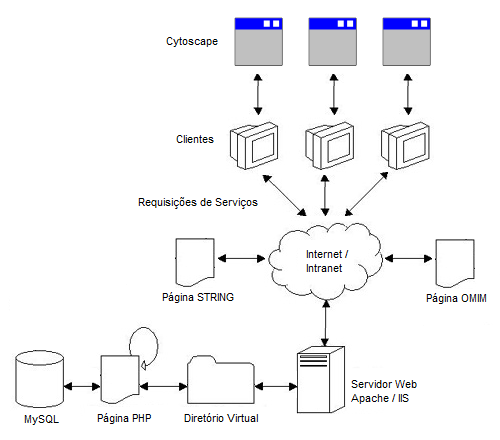
\includegraphics[scale=0.89]{imgs/ArquiteturaAplicacao}
	\caption{Diagrama de arquitetura da aplica��o}
	\label{fgr:ArquiteturaAplicacao}
\end{figure}

\section{Detalhamento da implementa��o}

Nessa se��o ser�o listadas e quando necess�rio detalhadas as funcionalidades que o sistema ir� oferecer aos usu�rios, para tornar o processo �gil e seguro.

\subsection{Algoritmo de extra��o dos dados}
\label{ssec:AlgoritmoExtracaoDados}

Express�es regulares podem ser definidas, ``como um m�todo formal de especificar um padr�o de texto'' \cite{Jargas:l08}. Por�m se formos defini-las de uma forma mais detalhada, podemos dizer que descrevem uma linguagem exclusivamente atrav�s de s�mbolos e caracteres com fun��es especiais, que agrupados entre si e com caracteres literais formam uma seq��ncia, uma express�o, que entre outros pode vir a ser interpretada por uma linguagem de programa��o, ou um editor de textos \cite{Jargas:l08, Lewis:l00}.

Ser� desenvolvida uma express�o regular para ser aplicada no relat�rio da doen�a que � apresentado pelo \emph{site} do OMIM. A express�o regular, como mostra a Figura \ref{fgr:AlgoritmoExtracao}, tem o objetivo de filtrar as palavras do texto que iniciem com letra mai�scula e que tenham apenas letras mai�sculas, n�meros ou tra�o. Embora o exemplo tenha sido desenvolvido em Python a express�o pode ser usada praticamente em qualquer linguagem de programa��o sem sofrer altera��es.

\begin{figure}[htp]
	\centering
	\framebox{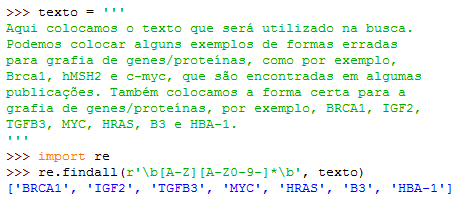
\includegraphics[scale=.8]{imgs/AlgoritmoExtracao}}
	\caption{Algoritmo de extra��o dos dados}
	\label{fgr:AlgoritmoExtracao}
\end{figure}

\subsection{Acesso aos sites do OMIM e do STRING}

Primeiramente ser�o testadas outras formas de acesso aos \emph{sites} do OMIM e do STRING, por exemplo, por \emph{Web Service}. Conforme os testes que ser�o realizados com as formas de acesso, ser�o escolhidas as maneiras mais otimizadas de acessar os dados (Atividades 1 e 3).

\subsection{Salvar e recuperar informa��es}

O sistema permitir� salvar e recuperar consultas de doen�as (Atividade 1), genes e prote�nas escolhidas (Atividade 3), sendo que esses dois itens anteriores transmitem os dados em formato texto, redes de intera��o de prote�nas (Atividade 6), sendo que esse � salvo em um arquivo do tipo XML, e a an�lise da ontologia g�nica (Atividade 9), que � salva no formato do software Cytoscape.

O sistema permitir� salvar em banco de dados as consultas realizadas pelo especialista, os genes e prote�nas j� consultados anteriormente, \emph{links} para redes de intera��o de prote�nas j� trabalhadas e informa��es do usu�rio para poder recuperar pesquisas personalizadas.

\subsection{Intera��o com o software Cytoscape}

A intera��o com o software Cytoscape se dar� atrav�s da possibilidade de baixar o software atrav�s do sistema, para caso o especialista ainda n�o o tenha instalado em sua m�quina, pesquisa por \emph{plug-ins} que poder�o vir a ser usados pelo especialista no software Cytoscape e a importa��o dos arquivos XML de redes de intera��o de prote�nas apresentados pelo sistema a ser desenvolvido (Atividade 7).

\section{Considera��es finais}

Nesse cap�tulo foram apresentados os artefatos desenvolvidos visando o desenvolvimento do sistema e algumas ferramentas existentes para a cria��o e execu��o de \emph{workflows} cient�ficos. Esse levantamento das ferramentas possibilitou o surgimento das id�ias para melhorar o fluxo de pesquisa dos usu�rios que foram apresentadas.

Criou-se um \emph{workflow} que visa demonstrar como ser� o fluxo de pesquisa no sistema, sendo esse explicado em detalhes, e foram desenvolvidos artefatos de software para demonstrar as intera��es dos usu�rios com o sistema. Tamb�m foi criado um esbo�o do algoritmo respons�vel por fazer a busca textual dos genes/prote�nas no relat�rio da doen�a e foram levantados detalhes a serem melhor avaliados como o acesso aos \emph{sites} do OMIM e do STRING, o armazenamento e manipula��o dos dados e a integra��o com o software Cytoscape.

No pr�ximo cap�tulo ser�o apresentados os artefatos e \emph{scripts} desenvolvidos com base no sistema e um manual do usu�rio.
	\chapter{Implementa��o}

Nesse cap�tulo ser�o apresentados o diagrama de arquitetura da aplica��o, o diagrama de componentes, trechos dos \emph{scripts} implementados e o \emph{workflow} cient�fico do sistema, sendo esses artefatos desenvolvidos com base em altera��es no projeto original. Os \emph{scripts} completos do sistema podem ser vistos no anexo A.

O sistema \emph{web} BioNet facilita o processo dos usu�rios de bioinform�tica permitindo que sejam pesquisadas redes de intera��o de prote�nas a partir de doen�as g�nicas, isso sem que seja necess�rio o uso direto das p�ginas \emph{web} do OMIM e do STRING. O sistema se encarrega de fazer a comunica��o com esses \emph{sites} e ainda permite acompanhar todo o processo que est� sendo realizado atrav�s de sua interface, podendo o usu�rio inclusive salvar e depois recuperar o processo executado.

\section{Diagrama de arquitetura da aplica��o}

Como j� havia sido descrito na subse��o \ref{ssec:ArquiteturaAplicacao} do cap�tulo \ref{cap:PropostaSoftware}, a arquitetura do sistema continuou sendo enxuta, por�m foi feita uma mudan�a na qual n�o � mais necess�ria a exist�ncia de um SGBD (Sistema Gerenciador de Banco de Dados). Como se constatou que os dados a serem armazenados s�o somente os passos executados, optou-se por permitir que o sistema salve e recupere esses dados a partir de um arquivo XML (\emph{Extensible Markup Language}), podendo o especialista manipular esse arquivo dentro do sistema. A Figura \ref{fgr:ArquiteturaSistema} mostra o diagrama de arquitetura do sistema modificado.

\begin{figure}[htp]
	\centering
	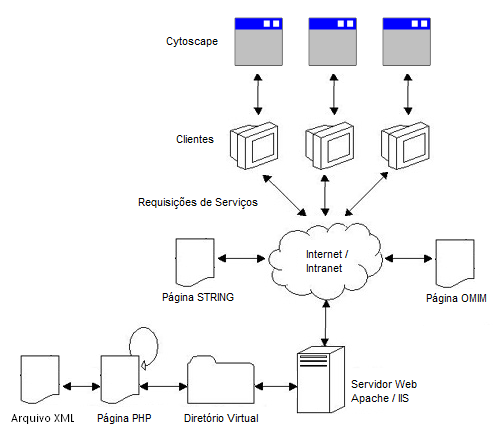
\includegraphics[width=.9\textwidth]{imgs/ArquiteturaSistema}
	\caption{Diagrama de arquitetura da aplica��o}
	\label{fgr:ArquiteturaSistema}
\end{figure}

\section{Implementa��o do sistema web}

O diagrama de componentes, mostrado na Figura \ref{fgr:DiagramaComponentes}, visa demonstrar como os componentes do sistema interagem entre si. Nas subse��es que seguem ser� explicado o que faz cada um dos componentes, apresentando alguns trechos de c�digo espec�ficos respons�veis pelas funcionalidades do sistema. A implementa��o reflete os passos do \emph{workflow} apresentado na subse��o \ref{ssec:WorkflowCientifico} do cap�tulo \ref{cap:PropostaSoftware}.

\begin{figure}[htp]
	\centering
	\framebox{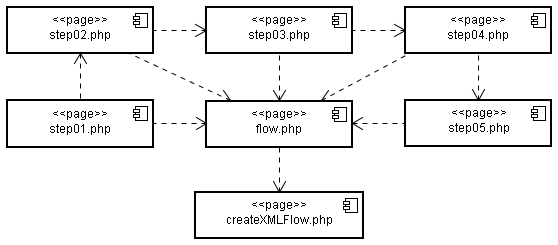
\includegraphics[width=.9\textwidth]{imgs/DiagramaComponentes}}
	\caption{Diagrama de Componentes}
	\label{fgr:DiagramaComponentes}
\end{figure}

\subsection{Pesquisa da doen�a}

O \emph{script} (step01.php) do primeiro componente se resume a um formul�rio HTML (\emph{HyperText Markup Language}) no qual o usu�rio digita o nome da doen�a que deseja encontrar e manda pesquisar.

\subsection{Busca e sele��o da doen�a}

O \emph{script} (step02.php) do segundo componente � respons�vel por fazer a busca e listar os resultados da pesquisa da doen�a, possibilitando ao usu�rio poder escolher a doen�a que est� procurando, conforme projetado no caso de uso da Figura \ref{fgr:CasoDeUso01}.

No \emph{Script} \ref{lst:step02t} o termo pesquisado, anteriormente, � recebido (linha 4), ent�o � informado o endere�o do \emph{Web Service} do \emph{site} do OMIM (linhas 5 e 6) e depois ele � instanciado no sistema (linha 7). Ap�s s�o capturadas as informa��es do \emph{proxy} (linha 8), � verificado se n�o houve erros (linha 9), os par�metros para a fun��o que traz os identificadores das doen�as com o termo s�o informados (linha 11) e ent�o a fun��o � chamada (linha 12). Tendo os identificadores armazenados em uma vari�vel, � feito um \emph{la�o} (linha 13) no qual s�o buscadas algumas informa��es das doen�as. Para isso, os par�metros para a fun��o que traz os nomes das doen�as s�o informados (linha 14) e a fun��o � chamada (linha 15), ap�s isso temos algumas informa��es da doen�a para ajudar o usu�rio na escolha (linhas 16 a 20).

\singlespace
\lstset{language=php}
\lstinputlisting[caption=step02.php (trecho), label=lst:step02t]{codes/step02-trecho.php}
\onehalfspace

\subsection{Visualiza��o do relat�rio e sele��o das prote�nas}

O \emph{script} (step03.php) do terceiro componente � respons�vel por apresentar o relat�rio da doen�a selecionada anteriormente e sugerir prote�nas encontradas, conforme projetado no caso de uso da Figura \ref{fgr:CasoDeUso01}.

No \emph{Script} \ref{lst:step03t} o identificador da doen�a selecionada, anteriormente, � recebido (linha 2) e ent�o � trazido o arquivo HTML da p�gina \emph{web} do \emph{site} do OMIM com o relat�rio da doen�a (linhas 3 e 4). Feito isso todo o conte�do da p�gina HTML, que vem na forma de um vetor, � organizado e colocado em uma vari�vel (linhas 5 e 6). Ap�s � criada uma vari�vel com a express�o regular (linha 7), conforme projetado na subse��o \ref{ssec:AlgoritmoExtracaoDados} do cap�tulo \ref{cap:PropostaSoftware} e que agora aparece melhorada e otimizada para a linguagem PHP, que � respons�vel por separar do relat�rio da doen�a as prote�nas, e ent�o a busca � realizada (linha 8).

Ent�o � feito um \emph{la�o} (linha 10) para testar todas as prote�nas. No primeiro teste (linhas 11 a 14) � verificado se o termo est� na lista de prote�nas encontradas. No segundo teste (linhas 15 a 18) � verificado se o termo encontrado est� na lista de termos a serem retirados (linha 9).

\singlespace
\lstset{language=php}
\lstinputlisting[caption=step03.php (trecho), label=lst:step03t]{codes/step03-trecho.php}
\onehalfspace

\pagebreak

No terceiro � verificado se o termo passou nos dois testes antes de ser adicionado a lista de prote�nas encontradas (linhas 19 e 20). Por fim o \emph{script} apresenta a lista de prote�nas encontradas e o relat�rio da doen�a (linhas 23 e 24).

O segundo teste (linhas 15 a 18) foi necess�rio devido � fun��o que executa a express�o regular (linha 7) n�o diferenciar termos em mai�sculas e min�sculas, fazendo com que sejam encontrados termos que n�o s�o prote�nas, como por exemplo, algumas \emph{tags} HTML e parte do relat�rio que n�o s�o prote�nas (linha 9).

\subsection{Sele��o das ocorr�ncias das prote�nas}

O \emph{script} (step04.php) do quarto componente � respons�vel por apresentar as ocorr�ncias das prote�nas selecionadas, em humanos, conforme projetado no caso de uso da Figura \ref{fgr:CasoDeUso01}.

No \emph{Script} \ref{lst:step04t} as prote�nas selecionadas s�o recebidas (linha 2) e organizadas em uma lista (linha 3). Ent�o � feito um \emph{la�o} (linha 4) que pega cada uma das prote�nas e busca o arquivo texto no \emph{site} do STRING com as ocorr�ncias da mesma em humanos (linhas 5 a 7) (\emph{species=9606} na linha 7 significa humanos), ent�o � realizado um teste (linha 8) para verificar se o arquivo de retorno � um vetor. Ap�s isso � feito um \emph{la�o} (linha 9) que pega cada item e separa o identificador da prote�na (linha 14) e a descri��o (linha 15), atrav�s da express�o regular (linha 10) que foi executada (linhas 11 e 12) e � respons�vel por separar as informa�oes que ser�o utilizadas.

\singlespace
\lstset{language=php}
\lstinputlisting[caption=step04.php (trecho), label=lst:step04t]{codes/step04-trecho.php}
\onehalfspace

\subsection{Visualiza��o da rede de intera��o da(s) prote�na(s)}

O \emph{script} (step05.php) do quinto componente � respons�vel por apresentar a rede de intera��o da(s) prote�na(s) e disponibilizar para \emph{download} seu arquivo XML, conforme projetado no caso de uso da Figura \ref{fgr:CasoDeUso01}.

No \emph{Script} \ref{lst:step05t} os identificadores das prote�nas selecionadas na quarta etapa s�o recebidos e armazenados em uma vari�vel (linha 2), ent�o � realizado um teste para verificar se o usu�rio selecionou alguma prote�na (linha 3), tendo selecionado alguma prote�na � feito um teste (linha 4) que verifica se uma �nica prote�na foi selecionada. Se apenas uma prote�na tiver sido selecionada (linha 4) o sistema montar� o \emph{link}, para a busca do arquivo texto no STRING, que cont�m o endere�o da imagem da rede de intera��o da prote�na (linhas 5 a 7).

\singlespace
\lstset{language=php}
\lstinputlisting[caption=step05.php (trecho), label=lst:step05t]{codes/step05-trecho.php}
\onehalfspace

Havendo mais de uma prote�na selecionada (linha 8) ser� montado o \emph{link} para a busca do arquivo texto no STRING, que cont�m o endere�o da imagem da rede de intera��o das prote�nas (linhas 9 a 19) colocando entre os identificadores das prote�nas um caractere especial (linha 12). Ent�o � feito um teste (linha 23) para verificar se o \emph{link} foi montado e em caso afirmativo � feita a busca do arquivo (linha 24). Dentro desse arquivo � tirado o endere�o da imagem da rede de intera��o da(s) prote�na(s) (linha 28) e atrav�s da express�o regular (linha 25) que foi executada (linhas 26 e 27), � separado o identificador da rede no STRING (linha 29) que permite buscar o arquivo XML, abrir a p�gina dos outros arquivos para \emph{download} e da rede de intera��o da(s) prote�na(s) na p�gina \emph{web} do STRING.

\subsection{Documenta��o do fluxo de pesquisa da doen�a}

O \emph{script} (flow.php) do sexto componente � respons�vel por documentar o fluxo de pesquisa da doen�a e controlar as altera��es nessa documenta��o.

O \emph{Script} \ref{lst:flowt} inicia com a inicializa��o de uma sess�o (linha 2), ent�o � realizado um teste para verificar se a sess�o \emph{fluxo} j� est� registrada (linha 3), se n�o estiver ent�o a sess�o � registrada (linha 4), caso esteja a vari�vel \emph{fluxo} (do tipo vetor) recebe o conte�do da sess�o com o mesmo nome (linha 6).

No primeiro teste a vari�vel \emph{textoUser} (respons�vel por capturar a entrada de dados do usu�rio no fluxo) recebe o conte�do de uma requisi��o identificada com o mesmo nome (linha 7), ap�s isso � realizado um teste para verificar se a vari�vel cont�m alguma informa��o (linha 8), caso contenha, esse valor � acrescentado ao final do vetor (linha 9). No segundo teste a vari�vel \emph{textoSoft} (respons�vel por capturar a entrada de dados do sistema no fluxo) recebe o conte�do de uma requisi��o identificada com o mesmo nome (linha 10), ap�s isso � realizado um teste para verificar se a vari�vel cont�m alguma informa��o (linha 11), caso contenha, esse valor � acrescentado ao final do vetor (linha 12).

No terceiro teste a vari�vel \emph{flowXML} (respons�vel por captura a entrada de dados do usu�rio de um arquivo XML de com um fluxo) recebe o conte�do de uma requisi��o identificada com o mesmo nome (linha 13), ap�s � realizado um teste para verificar se a vari�vel cont�m alguma informa��o (linha 14), caso contenha, s�o colocadas em vari�veis todas as informa��es do arquivo (linhas 15 a 18), ap�s s�o realizados outros teste para verificar se tamanho do arquivo � maior que zero, se o nome do arquivo cont�m algum texto e se o arquivo � do tipo XML (linhas 19 e 20), em caso afirmativo para todos os testes, o arquivo � renomeado e movido para junto dos \emph{scripts} do sistema (linhas 21 e 22). Ap�s isso � realizado mais um teste para verificar se o arquivo existe onde deveria estar (linha 23), caso exista o arquivo XML � aberto e carregado na vari�vel \emph{xml} (linhas 24 a 27) e ent�o � feito um \emph{la�o} para ler todos os nodos do arquivo e colocar os textos no vetor (linhas 28 e 29).

\singlespace
\lstset{language=php}
\lstinputlisting[caption=flow.php (trecho), label=lst:flowt]{codes/flow-trecho.php}
\onehalfspace

No quarto teste a vari�vel \emph{removeItem} (respons�vel por captura a indica��o de uma remo��o feita pelo usu�rio) recebe o conte�do de uma requisi��o identificada com o mesmo nome (linha 33), ap�s � realizado um teste para verificar se a vari�vel cont�m um n�mero v�lido do vetor (linha 34), caso contenha, � verificado se o vetor cont�m mais de um item (linha 35), se tiver, o item indicado pelo usu�rio � removido (linhas 36 e 37), caso n�o tenha, o vetor � todo apagado (linha 40).

No quinto teste a vari�vel \emph{limpaFluxo} (respons�vel por captura a indica��o da remo��o de todos os itens feita pelo usu�rio) recebe o conte�do de uma requisi��o identificada com o mesmo nome (linha 42), ap�s � realizado um teste para verificar se a vari�vel cont�m a confirma��o da remo��o (linha 43), em caso afirmativo, todo o conte�do do vetor � removido. Por fim, o vetor � gravado na vari�vel de sess�o com o mesmo nome (linha 45). Ap�s o vetor ter sido gravado ele pode ser visualizado com o comando \emph{print\_r(\$fluxo)}.

\subsection{Salvamento do fluxo de pesquisa da doen�a}

O \emph{script} (createXMLFlow.php) do s�timo componente � respons�vel por criar e disponibilizar para \emph{download} o arquivo XML que cont�m o fluxo de pesquisa da(s) doen�a(s).

O \emph{Script} \ref{lst:createXMLFlowt} inicia da mesma forma que o \emph{Script} \ref{lst:flowt} e das linhas 1 a 6 eles s�o id�nticos, para tanto essas linhas n�o ser�o explicadas novamente. Ap�s ter sido carregada ou criada a sess�o, na vari�vel \emph{filename} � armazenado o nome que ter� o arquivo a ser criado (linha 7), ent�o � criada a vari�vel que cont�m o arquivo XML (linhas 8 e 9), ap�s � criado o nodo \emph{flow} (linhas 10) e em seguida ele � adicionado ao arquivo (linha 11). Uma vez criado o nodo \emph{flow}, � feito um \emph{la�o} (linha 12) para criar um nodo \emph{step} para cada item do vetor contendo o valor desse item (linha 13) e depois adiciona-lo dentro do nodo \emph{flow} (linha 14). Feito isso o arquivo XML � salvo (linha 16).

As linhas 17 a 27 tem a �nica fun��o de fazer com que o sistema solicite um local para salvamento do arquivo na m�quina do usu�rio.

\subsection{Integra��o com o software Cytoscape}

A integra��o do sistema com o software Cytoscape ocorre atrav�s do arquivo XML da rede de intera��o da(s) prote�na(s) que � fornecido pelo quinto componente (step05.php) e que deve ser salvo para, posteriormente, ser importado pelo Cytoscape e utilizados os \emph{plug-ins} desejados.

\pagebreak

\singlespace
\lstset{language=php}
\lstinputlisting[caption=createXMLFlow.php (trecho), label=lst:createXMLFlowt]{codes/createXMLFlow-trecho.php}
\onehalfspace

\section{Workflow cient�fico do sistema web}

O \emph{workflow} cient�fico da Figura \ref{fgr:FluxoSoftware} visa demonstrar as etapas que o especialista precisa realizar no sistema \emph{web} para obter a(s) rede(s) de intera��o da(s) prote�na(s).

\begin{figure}[htp]
	\centering
	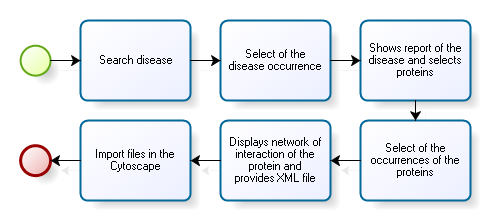
\includegraphics[scale=.75]{imgs/FluxoSoftware}
	\caption{Fluxo Software}
	\label{fgr:FluxoSoftware}
\end{figure}

O processo no sistema se inicia com a pesquisa da doen�a, como pode ser visto na Figura \ref{fgr:step01}. O usu�rio digita a doen�a que deseja encontrar e clica no bot�o \emph{Search}.

\begin{figure}[htp]
	\centering
	\framebox{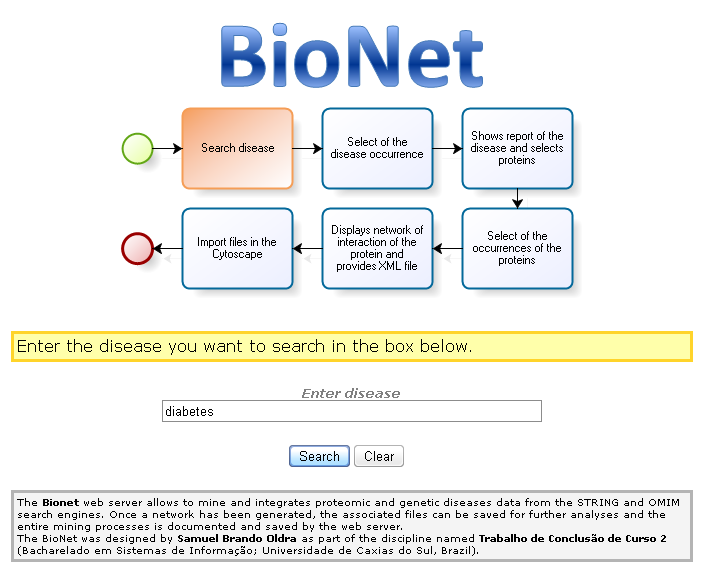
\includegraphics[width=.9\textwidth]{imgs/step01}}
	\caption{Procura da doen�a}
	\label{fgr:step01}
\end{figure}

Ent�o o sistema apresenta as ocorr�ncias de doen�as com aquele termo, assim como poderia ser feito no site do OMIM, para que o usu�rio escolha a doen�a que deseja visualizar e clica sobre seu \emph{link}, como mostra a Figura \ref{fgr:step02}.

\begin{figure}[ht]
	\centering
	\framebox{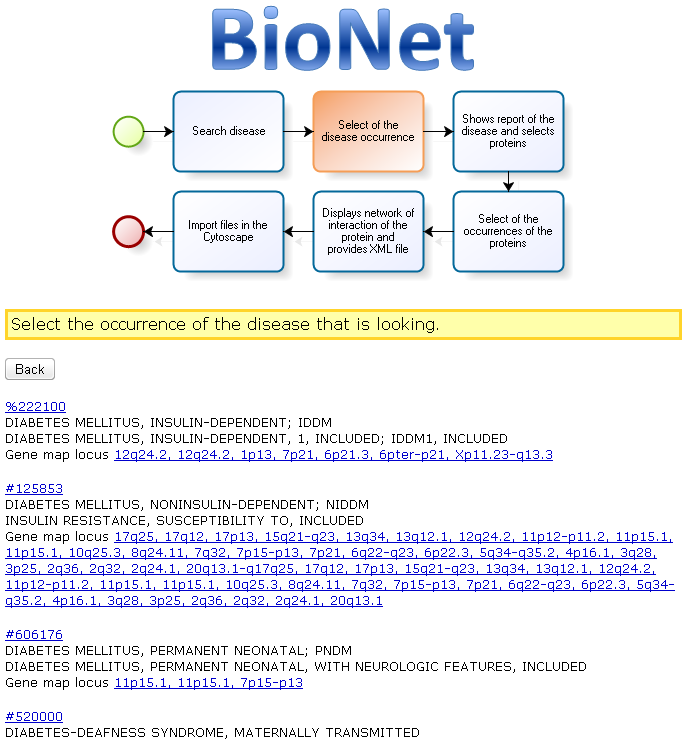
\includegraphics[width=.9\textwidth]{imgs/step02}}
	\caption{Seleciona a ocorr�ncia da doen�a}
	\label{fgr:step02}
\end{figure}

Ap�s isso, o sistema ir� apresentar o relat�rio da doen�a escolhida anteriormente (o mesmo apresentado pelo OMIM) e tamb�m ir� sugerir algumas prote�nas encontradas no relat�rio para que o usu�rio selecione as que deseja pesquisar, como mostra a Figura \ref{fgr:step03}.

Ent�o o usu�rio pode apagar as prote�nas que n�o deseja pesquisar da \emph{caixa de texto} e, acrescentar as que deseja pesquisar como o sistema n�o encontrou ou n�o est�o no relat�rio da doen�a, ap�s isso o usu�rio clica no bot�o \emph{Next} e o sistema ir� pesquisar as ocorr�ncias da(s) prote�na(s).

\begin{figure}[ht]
	\centering
	\framebox{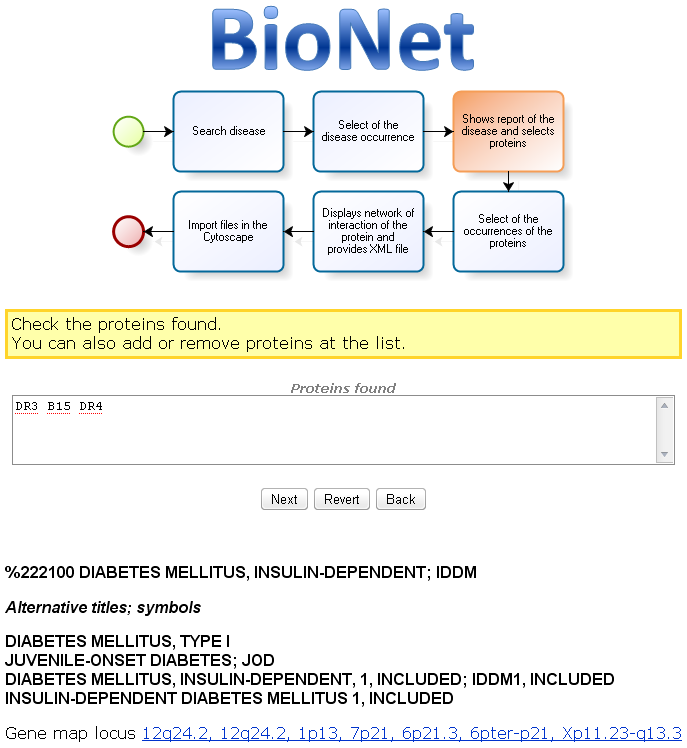
\includegraphics[width=.9\textwidth]{imgs/step03}}
	\caption{Apresenta relat�rio da doen�a e seleciona prote�nas}
	\label{fgr:step03}
\end{figure}

Na seq��ncia, o sistema ir� apresentar as ocorr�ncias de cada prote�na seleciona (em humanos), como mostra a Figura \ref{fgr:step04}, assim como s�o apresentadas no \emph{site} do STRING. O usu�rio ent�o seleciona as que deseja visualizar a rede de intera��o da(s) prote�na(s) e clica no bot�o \emph{Next} novamente.

\begin{figure}[ht]
	\centering
	\framebox{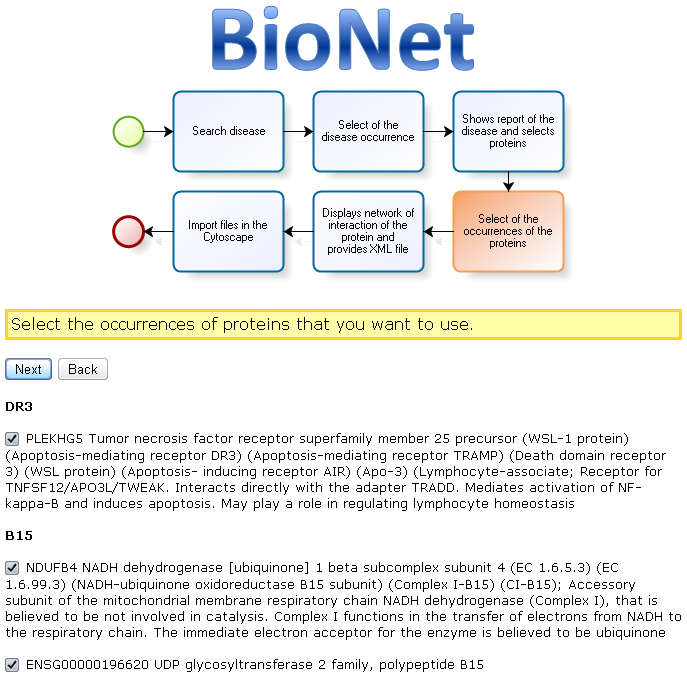
\includegraphics[width=.9\textwidth]{imgs/step04}}
	\caption{Seleciona as ocorr�ncias das prote�nas}
	\label{fgr:step04}
\end{figure}

\pagebreak

Por fim, o sistema apresenta a imagem da rede de intera��o da(s) prote�na(s), como pode ser visto na Figura \ref{fgr:step05}, deixa dispon�vel para \emph{download} o arquivo XML clicando no \emph{link} \emph{Download XML}, que pode ser usado no software Cytoscape, possibilita a visualiza��o dos outros arquivos que podem ser usados clicando no \emph{link} \emph{Other files} e clicando sobre a imagem o usu�rio ser� direcionado para a p�gina do STRING para poder realizar qualquer altera��o necess�ria.

\begin{figure}[htp]
	\centering
	\framebox{\includegraphics[width=.9\textwidth]{imgs/step05}}
	\caption{Apresenta rede de intera��o da prote�na e fornece arquivo XML}
	\label{fgr:step05}
\end{figure}

\pagebreak

Durante a execu��o do fluxo o usu�rio poder� observar que todos os passos est�o sendo documentados, como mostra a Figura \ref{fgr:flow}. Ent�o o usu�rio pode fazer outras pesquisas na seq��ncia, limpar o fluxo clicando no \emph{link} \emph{Clean flow}, salvar o processo clicando com o bot�o direito do \emph{mouse} no \emph{link Download flow} e escolhendo um local para o arquivo, adicionar ao fim do fluxo um outro executado anteriormente e/ou recuperar um fluxo clicando no bot�o \emph{Choose...}, localizando o arquivo XML do fluxo e ap�s clicando no bot�o \emph{Load}, adicionar coment�rios ao fluxo digitando a mensagem na caixa de texto \emph{User comments} e ap�s clicando no bot�o \emph{Add} e apagar etapas ou coment�rios desnecess�rios no fluxo clicando sobre o \emph{link} \emph{remove} ao lado do mesmo.

\begin{figure}[htp]
	\centering
	\framebox{\includegraphics[scale=0.8]{imgs/flow}}
	\caption{Fluxo de pesquisa}
	\label{fgr:flow}
\end{figure}

\pagebreak

\section{Considera��es finais}

Nesse cap�tulo foram apresentados os artefatos e \emph{scripts} desenvolvidos com base no sistema e um manual de funcionamento do sistema.

Durante o desenvolvimento do sistema, houve problemas com o sistema e mudan�as na proposta de software, sendo essas explicadas a seguir. Optou-se por salvar os fluxos de pesquisa desenvolvidos pelo especialista em arquivos XML ao inv�s de em um SGBD (Sistema Gerenciador de Banco de Dados), visando deixar a cargo do especialista a manuten��o de suas pesquisas, foram utilizadas formas de acesso diferentes das que haviam sido propostas, sendo usadas �s indicadas pelos \emph{sites} do OMIM e  do STRING na maioria das ocasi�es, o \emph{workflow} do sistema foi modificado para deixar a escolha de uma ou mais prote�nas transparente ao usu�rio, e existe um problema que n�o pode ser resolvido com rela��o � busca de prote�nas n�o existentes no STRING. Tamb�m podemos mencionar que houve dificuldades com rela��o � hospedagem do sistema, sendo o atendimento e solicita��es demorados.

No pr�ximo cap�tulo ser�o apresentados os estudos de caso realizados com profissionais da �rea da biologia e da inform�tica e suas opini�es com rela��o ao sistema.
	\chapter{Estudo de caso}

Nesse cap�tulo ser�o apresentados os estudos de caso realizados com profissionais da �rea da inform�tica e da biologia, a avalia��o deles do sistema e minha avalia��o como observador. O formul�rio de pesquisa pode ser visto no anexo B.

\section{Primeiro estudo de caso}

O primeiro estudo de caso foi realizado com o Prof. MSc. Daniel Lu�s Notari, profissional da �rea de inform�tica, no dia 30 de novembro de 2009 �s 17 horas e foi utilizado o navegador \emph{web} ``Firefox''.

No estudo, iniciou a pesquisa procurando pelo termo ``alergics'', recebendo como resposta que o item n�o foi encontrado, na seq��ncia procurou pelos termos ``sarampo'', ``cachumba'' e ``caxumba'' obtendo a mesma resposta, j� que esses quatro termos n�o existem na base de dados do OMIM. Ent�o procurou pelo termo ``malaria'', obtendo assim a lista de ocorr�ncias de doen�as com esse termo. Selecionou a doen�a com o identificador ``+109270'' e com descri��o principal ``SOLUTE CARRIER FAMILY 4 (ANION EXCHANGER), MEMBER 1; SLC4A1''. Ap�s isso foram apresentadas a descri��o da doen�a e algumas sugest�es de prote�nas encontradas na mesma, ent�o foram removidas algumas prote�nas e termos que n�o eram prote�nas, acrescentou-se a prote�na ``COX-1'' e realizou a pesquisa pelas prote�nas ``SLC4A1'', ``BND3'', ``EMPB3'', ``EPB3'', ``AE1'' e ``COX-1'', obtendo assim a lista de ocorr�ncias das prote�nas em humanos. Ent�o selecionou a �nica ocorr�ncia da prote�na ``SLC4A1'' e clicou para prosseguir, podendo assim visualizar a rede de intera��o da prote�na, conforme mostra a Figura \ref{fgr:PrimeiroEstudoCasoSTRING}. Abaixo a descri��o da prote�na selecionada:

\begin{itemize}
	\item \emph{SLC4A1 Band 3 anion transport protein (Anion exchange protein 1) (AE 1) (Solute carrier family 4 member 1) (CD233 antigen); Band 3 is the major integral glycoprotein of the erythrocyte membrane. Band 3 has two functional domains. Its integral domain mediates a 1:1 exchange of inorganic anions across the membrane, whereas its cytoplasmic domain provides binding sites for cytoskeletal proteins, glycolytic enzymes, and hemoglobin}.
\end{itemize}

\begin{figure}[ht]
	\centering
	\framebox{\includegraphics[width=.9\textwidth]{imgs/PrimeiroEstudoCasoSTRING}}
	\caption{Primeiro estudo de caso rede STRING}
	\label{fgr:PrimeiroEstudoCasoSTRING}
\end{figure}

Ap�s isso realizou o \emph{download} do arquivo XML da rede de intera��o da prote�na, importou o mesmo no software Cytoscape, conforme mostra a Figura \ref{fgr:PrimeiroEstudoCasoCytoscape}, e realizou alguns testes. Depois voltou ao sistema, realizou o \emph{download} do arquivo XML do fluxo e respondeu ao question�rio de avalia��o do sistema.

\begin{figure}[ht]
	\centering
	\includegraphics[width=.9\textwidth]{imgs/PrimeiroEstudoCasoCytoscape}
	\caption{Primeiro estudo de caso rede Cytoscape}
	\label{fgr:PrimeiroEstudoCasoCytoscape}
\end{figure}

Na avalia��o realizada pelo Prof. MSc. Daniel Lu�s Notari o sistema foi considerado entre �timo e bom, tendo o item com pior avalia��o sido considerado regular, no caso, a busca de prote�nas no relat�rio da doen�a.

\section{Segundo estudo de caso}

O segundo estudo de caso foi realizado com a Profa. Dra. Helena Graziottin Ribeiro, profissional da �rea de inform�tica, no dia 1� de dezembro de 2009 �s 17 horas e 30 minutos e foi utilizado o navegador \emph{web} ``Firefox''.

No estudo, iniciou a pesquisa procurando pelo termo ``down syndrome'', obtendo assim a lista de ocorr�ncias de doen�as com esse termo. Selecionou a doen�a com o identificador ``\#190685'' e com descri��o principal ``DOWN SYNDROME''. Ap�s isso foram apresentadas a descri��o da doen�a e algumas sugest�es de prote�nas encontradas na mesma, ent�o foram removidas algumas prote�nas e termos que n�o eram prote�nas e realizou a pesquisa pelas prote�nas ``DOWN'', ``REGION'', ``DCR'', ``DSCR'', ``GATA1'', ``ALL'', ``AML'', ``APP'', ``DS'', ``T4'', ``CH'' e ``TSH'', obtendo assim a lista de ocorr�ncias das prote�nas em humanos. Durante essa pesquisa das ocorr�ncias das prote�nas, como nem todos os termos pesquisados eram prote�nas o sistema apresentou ``alertas'' para os termos ``DOWN'' e ``DSCR''. Ent�o selecionou seis ocorr�ncias da prote�na ``REGION'' (que a princ�pio n�o � uma prote�na) e clicou para prosseguir, podendo assim visualizar a rede de intera��o da prote�na, conforme mostra a Figura \ref{fgr:SegundoEstudoCasoSTRING}. Abaixo as descri��es das seis prote�nas selecionadas:

\begin{itemize}
	\item \emph{DSCR10 Down syndrome critical region protein 10};
	\item \emph{CECR6 Cat eye syndrome critical region protein 6};
	\item \emph{DSCR4 Down syndrome critical region protein 4 (Down syndrome critical region protein B)};
	\item \emph{DSCR8 Down syndrome critical region protein 8 (Malignant melanoma-associated protein 1) (MMA-1) (MTAG2 protein)};
	\item \emph{DSCR6 Down syndrome critical region protein 6};
	\item \emph{DSCR9 Down syndrome critical region protein 9}.
\end{itemize}

\begin{figure}[ht]
	\centering
	\framebox{\includegraphics[width=.9\textwidth]{imgs/SegundoEstudoCasoSTRING}}
	\caption{Segundo estudo de caso rede STRING}
	\label{fgr:SegundoEstudoCasoSTRING}
\end{figure}

Ap�s isso realizou o \emph{download} do arquivo XML da rede de intera��o das prote�nas, mas o mesmo n�o foi importado no Cytoscape por a Profa. n�o o ter instalado em sua m�quina. Depois voltou ao sistema, realizou o \emph{download} do arquivo XML do fluxo, limpou o fluxo, fez \emph{upload} do arquivo XML do fluxo no sistema, inseriu um coment�rio no fluxo, depois o apagou e, por fim, respondeu ao question�rio de avalia��o do sistema.

Na avalia��o realizada pela Profa. Dra. Helena Graziottin Ribeiro o sistema foi considerado bom, tendo o item com melhor avalia��o sido considerado �timo, no caso, a rede de intera��o da prote�na apresentada como resultado. Nos coment�rio de sua avalia��o tamb�m destacou que a visualiza��o do fluxo durante toda a pesquisa ajuda a saber em que fase dela se est� trabalhando, sendo isso de grande import�ncia.

\section{Terceiro estudo de caso}

O terceiro estudo de caso foi realizado com a Profa. MSc. Scheila de Avila e Silva, profissional da �rea de biologia, no dia 2 de dezembro de 2009 �s 16 horas e 30 minutos e foi utilizado o navegador \emph{web} ``Firefox''.

No estudo, iniciou a pesquisa procurando pelo termo ``turner syndrome'', obtendo assim a lista de ocorr�ncias de doen�as com esse termo. Selecionou a doen�a com o identificador ``\#163950'' e com descri��o principal ``NOONAN SYNDROME 1; NS1''. Ap�s isso foram apresentadas a descri��o da doen�a e algumas sugest�es de prote�nas encontradas na mesma, ent�o foram removidos termos que n�o eram prote�nas e realizou a pesquisa pelas prote�nas ``NS1'', ``PTPN11'', ``SHP2'', ``SH2'', ``NF1'', ``NFNS'', ``KRAS'' e ``NS3'', obtendo assim a lista de ocorr�ncias das prote�nas em humanos. Durante essa pesquisa das ocorr�ncias das prote�nas, como um dos termos pesquisados n�o era uma prote�na (``TPN11'') o sistema apresentou um ``alerta'' para o mesmo. Ent�o selecionou quatro ocorr�ncias de prote�nas, duas da ``NS1'', uma da ``NF1'' e uma da ``KRAS'', e clicou para prosseguir, podendo assim visualizar a rede de intera��o da prote�na, conforme mostra a Figura \ref{fgr:TerceiroEstudoCasoSTRING}. Abaixo as descri��es das quatro prote�nas selecionadas:

\begin{itemize}
	\item \emph{CPSF4 Cleavage and polyadenylation specificity factor subunit 4 (Cleavage and polyadenylation specificity factor 30 kDa subunit) (CPSF 30 kDa subunit) (NS1 effector domain-binding protein 1) (Neb-1) (No arches homolog); Component of the cleavage and polyadenylation specificity factor (CPSF) complex that play a key role in pre-mRNA 3'-end formation, recognizing the AAUAAA signal sequence and interacting with poly(A) polymerase and other factors to bring about cleavage and poly(A) addition. CPSF4 binds RNA polymers with a preference for poly(U)};
	\item \emph{PTPN11 Tyrosine-protein phosphatase non-receptor type 11 (EC 3.1.3.48) (Protein-tyrosine phosphatase 2C) (PTP-2C) (PTP-1D) (SH-PTP3) (SH- PTP2) (SHP-2) (Shp2); Acts downstream of various receptor and cytoplasmic protein tyrosine kinases to participate in the signal transduction from the cell surface to the nucleus};
	\item \emph{NF1 Neurofibromin (Neurofibromatosis-related protein NF-1) [Contains: Neurofibromin truncated]; Stimulates the GTPase activity of Ras. NF1 shows greater affinity for Ras GAP, but lower specific activity. May be a regulator of Ras activity};
	\item \emph{KRAS GTPase KRas precursor (K-Ras 2) (Ki-Ras) (c-K-ras) (c-Ki-ras); Ras proteins bind GDP/GTP and possess intrinsic GTPase activity}.
\end{itemize}

\begin{figure}[ht]
	\centering
	\framebox{\includegraphics[width=.9\textwidth]{imgs/TerceiroEstudoCasoSTRING}}
	\caption{Terceiro estudo de caso rede STRING}
	\label{fgr:TerceiroEstudoCasoSTRING}
\end{figure}

Ap�s isso realizou o \emph{download} do arquivo XML da rede de intera��o das prote�nas, mas o mesmo n�o foi importado no Cytoscape por a Profa. n�o o ter instalado em sua m�quina. Depois voltou ao sistema, realizou o \emph{download} do arquivo XML do fluxo e respondeu ao question�rio de avalia��o do sistema.

Na avalia��o realizada pela Profa. MSc. Scheila de Avila e Silva o sistema foi considerado �timo, tendo o item com com pior avalia��o sido considerado bom, no caso, a busca de prote�nas no relat�rio da doen�a. Nos coment�rios de sua avalia��o destacou que o sistema � �til para bi�logos que trabalham com redes e rela��es de informa��es de diferentes bancos de dados, e que o trabalho deveria ser ampliado para integra��o de informa��es de outros bancos de dados.

\section{Quarto estudo de caso}

O quarto estudo de caso foi realizado com o Prof. Dr. Diego Bonatto, profissional da �rea de biologia, no dia 3 de dezembro de 2009 �s 14 horas e 30 minutos e foi utilizado o navegador \emph{web} ``Firefox''. Nas subse��es que seguem ser�o apresentadas as tr�s pesquisas realizadas.

\subsection{Primeira pesquisa}

No primeiro estudo, iniciou a pesquisa procurando pelo termo ``huntington'', obtendo assim a lista de ocorr�ncias de doen�as com esse termo. Selecionou a doen�a com o identificador ``\#143100'' e com descri��o principal ``HUNTINGTON DISEASE; HD''. Ap�s isso foram apresentadas a descri��o da doen�a e algumas sugest�es de prote�nas encontradas na mesma, ent�o foram removidos os termos que n�o eram prote�nas e realizou a pesquisa pelas prote�nas ``HD'', ``HTT'', ``MRI'', ``XL'', ``DM1'', ``NF1'', ``NF2'', ``D4S10'', ``SE'', ``G8'' e ``MMSE'', obtendo assim a lista de ocorr�ncias das prote�nas em humanos. Durante essa pesquisa das ocorr�ncias das prote�nas, como nem todos os termos pesquisados eram prote�nas o sistema apresentou ``alertas'' para os termos ``D4S10'' e ``MMSE''. Ent�o selecionou quatorze ocorr�ncias de prote�nas, quatro da ``HD'', uma da ``HTT'', uma da ``MRI'', uma da ``XL'', uma da ``DM1'', duas da ``NF1'', uma da ``NF2'', duas da ``SE'' e um da ``G8'', e clicou para prosseguir, podendo assim visualizar a rede de intera��o das prote�nas, conforme mostra a Figura \ref{fgr:QuartoEstudoCasoSTRING1}. Abaixo as descri��es das quatorze prote�nas selecionadas:

\pagebreak

\begin{itemize}
	\item \emph{OPTN Optineurin (Optic neuropathy-inducing protein) (E3-14.7K-interacting protein) (FIP-2) (Huntingtin-interacting protein HYPL) (NEMO-related protein) (Transcription factor IIIA-interacting protein) (TFIIIA- IntP); Plays a neuroprotective role in the eye and optic nerve. Probably part of the TNF-alpha signaling pathway that can shift the equilibrium toward induction of cell death. May act by regulating membrane trafficking and cellular morphogenesis via a complex that contains Rab8 and hungtingtin (HD). May constitute a cellular target for adenovirus E3 14.7, an inhibitor of TNF-alpha func [\ldots]};
	\item \emph{HDDC3 HD domain-containing protein 3};
	\item \emph{PTPN23 Tyrosine-protein phosphatase non-receptor type 23 (EC 3.1.3.48) (His- domain-containing protein tyrosine phosphatase) (HD-PTP) (Protein tyrosine phosphatase TD14) (PTP-TD14); May act as a negative regulator of Ras-mediated mitogenic activity};
	\item \emph{FBXO16 Zinc finger protein 395 (Papillomavirus-binding factor) (Papillomavirus regulatory factor 1) (PRF-1) (Huntington disease gene regulatory region-binding protein 2) (HDBP-2) (HD gene regulatory region-binding protein 2) (HD-regulating factor 2) (HDRF-2); Probably recognizes and binds to some phosphorylated proteins and promotes their ubiquitination and degradation};
	\item \emph{SLC6A4 Sodium-dependent serotonin transporter (5HT transporter) (5HTT); Terminates the action of serotonin by its high affinity sodium-dependent reuptake into presynaptic terminals};
	\item \emph{C7orf49 Uncharacterized protein C7orf49; May act as a regulator of proteasome (By similarity)};
	\item \emph{RTN4 Reticulon-4 (Neurite outgrowth inhibitor) (Nogo protein) (Foocen)\\(Neuroendocrine-specific protein) (NSP) (Neuroendocrine-specific protein C homolog) (RTN-x) (Reticulon-5); Potent neurite growth inhibitor in vitro and plays a role both in the restriction of axonal regeneration after injury and in structural plasticity in the CNS. Isoform 2 reduces the anti-apoptotic activity of Bcl-xl and Bcl-2. This is likely consecutive to their change in subcellular location, from the mitochondria to the endoplasmic reticulum, after binding and sequestration. Isoform 2 and isoform 3 inhibit BACE1 ac [\ldots]};
	\item \emph{DMPK Myotonin-protein kinase (EC 2.7.11.1) (Myotonic dystrophy protein kinase) (MDPK) (DM-kinase) (DMK) (DMPK) (MT-PK); Critical to the modulation of cardiac contractility and to the maintenance of proper cardiac conduction activity. Phosphorylates phospholamban};
	\item \emph{NFIC Nuclear factor 1 C-type (Nuclear factor 1/C) (NF1-C) (NFI-C) (NF-I/C) (CCAAT-box-binding transcription factor) (CTF) (TGGCA-binding protein); Recognizes and binds the palindromic sequence 5'-TTGGCNNNNNGCCAA-3' present in viral and cellular promoters and in the origin of replication of adenovirus type 2. These proteins are individually capable of activating\\transcription and replication (By similarity)};
	\item \emph{APOBEC1 C->U-editing enzyme APOBEC-1 (EC 3.5.4.-) (Apolipoprotein B mRNA- editing enzyme 1) (HEPR); Catalytic component of the apolipoprotein B mRNA editing enzyme complex which is responsible for the postranscriptional editing of a CAA codon for Gln to a UAA codon for stop in the APOB mRNA. Also involved in CGA (Arg) to UGA (Stop) editing in the NF1 mRNA};
	\item \emph{NF2 Merlin (Moesin-ezrin-radixin-like protein) (Neurofibromin-2) (Schwannomin) (Schwannomerlin); Probably acts as a membrane stabilizing protein. May inhibit PI3 kinase by binding to AGAP2 and impairing its stimulating activity};
	\item \emph{EZH2 Enhancer of zeste homolog 2 (ENX-1); Polycomb group (PcG) protein. Catalytic subunit of the PRC2/EED-EZH2 complex, which methylates `Lys-9' and `Lys-27' of histone H3, leading to transcriptional repression of the affected target gene. Able to mono-, di- and trimethylate `Lys-27' of histone H3 to form H3K27me1, H3K27me2 and H3K27me3, respectively. Compared to EZH2-containing complexes, it is more abundant in embryonic stem cells and plays a major role in forming H3K27me3, which is required for embryonic stem cell identity and proper differentiation. The PRC2/EED-EZH2 complex may also se [\ldots]};
	\item \emph{FUT1 Galactoside 2-alpha-L-fucosyltransferase 1 (EC 2.4.1.69)(GDP-L-fucose:\\beta-D-galactoside 2-alpha-L-fucosyltransferase 1) (Alpha(1,2)FT 1) (Fucosyltransferase 1) (Blood group H alpha 2- fucosyltransferase); Creates a soluble precursor oligosaccharide FuC-alpha ((1,2)Galbeta-) called the H antigen which is an essential substrate for the final step in the soluble A and B antigen synthesis pathway. H and Se enzymes fucosylate the same acceptor substrates but exhibit different Km values};
	\item \emph{G8 Protein G8}.
\end{itemize}

\begin{figure}[ht]
	\centering
	\framebox{\includegraphics[width=.9\textwidth]{imgs/QuartoEstudoCasoSTRING1}}
	\caption{Quarto estudo de caso rede STRING primeira pesquisa}
	\label{fgr:QuartoEstudoCasoSTRING1}
\end{figure}

Ap�s isso realizou o \emph{download} do arquivo XML da rede de intera��o da prote�na, importou o mesmo no software Cytoscape, mas devido as prote�nas da rede n�o terem nenhuma liga��o o Cytoscape apresentou uma tela em branco.

\subsection{Segunda pesquisa}

No segundo estudo, iniciou a pesquisa procurando pelo termo ``charcot marie'', obtendo assim a lista de ocorr�ncias de doen�as com esse termo. Selecionou a doen�a com o identificador ``\#604563'' e com descri��o principal ``CHARCOT-MARIE-TOOTH DISEASE, TYPE 4B2; CMT4B2''. Ap�s isso foram apresentadas a descri��o da doen�a e algumas sugest�es de prote�nas encontradas na mesma, ent�o foram removidos os termos que n�o eram prote�nas e realizou a pesquisa pelas prote�nas ``CMT4B2'', ``SBF2'', ``CMT4B1'', ``MTMR2'', ``CMT'', ``CMT4A'', ``CSF'', ``CMT4B'' e ``MTMR13'', obtendo assim a lista de ocorr�ncias das prote�nas em humanos. Durante essa pesquisa das ocorr�ncias das prote�nas, como um dos termos pesquisados n�o era uma prote�na (``CMT4A'') o sistema apresentou um ``alerta'' para o mesmo. Ent�o selecionou quatorze ocorr�ncias de prote�nas, uma da ``CMT4B2'', uma da ``SBF2'', uma da ``CMT4B1'', uma da ``MTMR2'', uma da ``CMT'', sete da ``CSF'', uma da ``CMT4B'' e uma da ``MTMR13'', e clicou para prosseguir, podendo assim visualizar a rede de intera��o da prote�na, conforme mostra a Figura \ref{fgr:QuartoEstudoCasoSTRING2}. Abaixo as descri��es das prote�nas selecionadas, sendo que as repetidas n�o ser�o citadas mais de uma vez:

\begin{itemize}
	\item \emph{SBF2 Myotubularin-related protein 13 (SET-binding factor 2); Not known};
	\item \emph{MTMR2 Myotubularin-related protein 2 (EC 3.1.3.-); Phosphatase that acts on lipids with a phosphoinositol headgroup. Has phosphatase activity towards phosphatidylinositol- 3-phosphate and phosphatidylinositol-3,5-bisphosphate};
	\item \emph{ENSG00000181464 CMT duplicated region transcript 1};
	\item \emph{CSF2RA Granulocyte-macrophage colony-stimulating factor receptor alpha chain precursor (GM-CSF-R-alpha) (GMR) (CD116 antigen) (CDw116); Low\\affinity receptor for granulocyte-macrophage colony- stimulating factor. Transduces a signal that results in the proliferation, differentiation, and functional activation of hematopoietic cells};
	\item \emph{NFATC2 Nuclear factor of activated T-cells, cytoplasmic 2 (T cell transcription factor NFAT1) (NFAT pre-existing subunit) (NF-ATp); Plays a role in the inducible expression of cytokine genes in T-cells, especially in the induction of the IL-2, IL-3, IL-4, TNF-alpha or GM-CSF};
	\item \emph{CSF3R Granulocyte colony-stimulating factor receptor precursor (G-CSF-R) (CD114 antigen); Receptor for granulocyte colony-stimulating factor (CSF3). In addition it may function in some adhesion or recognition events at the cell surface};
	\item \emph{CBFB Core-binding factor subunit beta (CBF-beta) (Polyomavirus enhancer- binding protein 2 beta subunit) (PEBP2-beta) (PEA2-beta) (SL3-3 enhancer factor 1 beta subunit) (SL3/AKV core-binding factor beta subunit); CBF binds to the core site, 5'-PYGPYGGT-3', of a number of enhancers and promoters, including murine leukemia virus, polyomavirus enhancer, T-cell receptor enhancers, LCK, IL-3 and GM-CSF promoters. CBFB enhances DNA binding by RUNX1};
	\item \emph{CSF2 Granulocyte-macrophage colony-stimulating factor precursor (GM-CSF) (Colony-stimulating factor) (CSF) (Sargramostim) (Molgramostin); Cytokine that stimulates the growth and differentiation of hematopoietic precursor cells from various lineages, including granulocytes, macrophages, eosinophils and erythrocytes};
	\item \emph{CSF1R Macrophage colony-stimulating factor 1 receptor precursor (EC 2.7.10.1) (CSF-1-R) (Fms proto-oncogene) (c-fms) (CD115 antigen); Protein tyrosine-kinase transmembrane receptor for CSF1 and IL34};
	\item \emph{IL10 Interleukin-10 precursor (IL-10) (Cytokine synthesis inhibitory factor) (CSIF); Inhibits the synthesis of a number of cytokines, including IFN-gamma, IL-2, IL-3, TNF and GM-CSF produced by activated macrophages and by helper T-cells}.
\end{itemize}

\begin{figure}[htp]
	\centering
	\framebox{\includegraphics[width=.9\textwidth]{imgs/QuartoEstudoCasoSTRING2}}
	\caption{Quarto estudo de caso rede STRING segunda pesquisa}
	\label{fgr:QuartoEstudoCasoSTRING2}
\end{figure}

Ap�s isso realizou o \emph{download} do arquivo XML da rede de intera��o da prote�na, importou o mesmo no software Cytoscape, conforme mostra a Figura \ref{fgr:QuartoEstudoCasoCytoscape2}, e realizou alguns testes. Depois voltou ao sistema e inseriu um coment�rio no fluxo antes de realizar o terceiro estudo de caso.

\begin{figure}[htp]
	\centering
	\includegraphics[width=.9\textwidth]{imgs/QuartoEstudoCasoCytoscape2}
	\caption{Quarto estudo de caso rede Cytoscape segunda pesquisa}
	\label{fgr:QuartoEstudoCasoCytoscape2}
\end{figure}

\subsection{Terceira pesquisa}

No terceiro estudo, iniciou a pesquisa procurando pelo termo ``cockayne'', obtendo assim a lista de ocorr�ncias de doen�as com esse termo. Selecionou a doen�a com o identificador ``\#216400'' e com descri��o principal ``COCKAYNE SYNDROME, TYPE A; CSA''. Ap�s isso foram apresentadas a descri��o da doen�a e algumas sugest�es de prote�nas encontradas na mesma, ent�o foram removidos os termos que n�o eram prote�nas e realizou a pesquisa pelas prote�nas ``CSA'', ``CKN1'', ``ERCC8'', ``CSB'', ``ERCC6'', ``ERCC3'', ``ERCC2'', ``ERCC5'' e ``COFS'', obtendo assim a lista de ocorr�ncias das prote�nas em humanos. Ent�o selecionou treze ocorr�ncias de prote�nas, cinco da ``CSA'', uma da ``CKN1'', uma da ``ERCC8'', uma da ``CSB'', uma da ``ERCC6'', uma da ``ERCC3'', uma da ``ERCC2'', uma da ``ERCC5'' e uma da ``COFS'', e clicou para prosseguir, podendo assim visualizar a rede de intera��o da prote�na, conforme mostra a Figura \ref{fgr:QuartoEstudoCasoSTRING3}. Abaixo as descri��es das prote�nas selecionadas, sendo que as repetidas n�o ser�o citadas mais de uma vez:

\begin{itemize}
	\item \emph{ERCC8 DNA excision repair protein ERCC-8 (Cockayne syndrome WD repeat protein CSA); Involved in transcription};
	\item \emph{COPS3 COP9 signalosome complex subunit 3 (Signalosome subunit 3) (SGN3) (JAB1-containing signalosome subunit 3); Component of the COP9 signalosome complex (CSN), a complex involved in various cellular and developmental processes. The CSN complex is an essential regulator of the ubiquitin (Ubl) conjugation pathway by mediating the deneddylation of the cullin subunits of SCF-type E3 ligase complexes, leading to decrease the Ubl ligase activity of SCF-type complexes such as SCF, CSA or DDB2. The complex is also involved in phosphorylation of p53/TP53, c-jun/JUN, IkappaBalpha/NFKBIA, ITPK1 and I [\ldots]};
	\item \emph{COPS4 COP9 signalosome complex subunit 4 (Signalosome subunit 4) (SGN4) (JAB1-containing signalosome subunit 4); Component of the COP9 signalosome complex (CSN), a complex involved in various cellular and developmental processes. The CSN complex is an essential regulator of the ubiquitin (Ubl) conjugation pathway by mediating the deneddylation of the cullin subunits of SCF-type E3 ligase complexes, leading to decrease the Ubl ligase activity of SCF-type complexes such as SCF, CSA or DDB2. The complex is also involved in phosphorylation of p53/TP53, c-jun/JUN, IkappaBalpha/NFKBIA, ITPK1 and I [\ldots]};
	\item \emph{HSPA9 Stress-70 protein, mitochondrial precursor (75 kDa glucose-regulated protein) (GRP 75) (Peptide-binding protein 74) (PBP74) (Mortalin) (MOT); Implicated in the control of cell proliferation and cellular aging. May also act as a chaperone};
	\item \emph{COPS6 COP9 signalosome complex subunit 6 (Signalosome subunit 6) (SGN6) (JAB1-containing signalosome subunit 6) (Vpr-interacting protein) (hVIP) (MOV34 homolog); Component of the COP9 signalosome complex (CSN), a complex involved in various cellular and developmental processes. The CSN complex is an essential regulator of the ubiquitin (Ubl) conjugation pathway by mediating the deneddylation of the cullin subunits of SCF-type E3 ligase complexes, leading to decrease the Ubl ligase activity of SCF-type complexes such as SCF, CSA or DDB2. The complex is also involved in phosphorylation of p53/ [\ldots]};
	\item \emph{ERCC6 DNA excision repair protein ERCC-6 (EC 3.6.1.-) (ATP-dependent helicase ERCC6) (Cockayne syndrome protein CSB); Is involved in the\\preferential repair of active genes. Presumed DNA or RNA unwinding function. Corrects the UV survival and RNA synthesis after UV exposure of\\Cockayne syndrome complementation group B};
	\item \emph{ERCC3 TFIIH basal transcription factor complex helicase XPB subunit (EC 3.6.1.-) (Basic transcription factor 2 89 kDa subunit) (BTF2-p89) (TFIIH 89 kDa subunit) (DNA-repair protein complementing XP-B cells) (Xeroderma pigmentosum group B-complementing protein); ATP-dependent 3'-5' DNA helicase, component of the core- TFIIH basal transcription factor, involved in nucleotide excision repair (NER) of DNA and, when complexed to CAK, in RNA transcription by RNA polymerase II. Acts by opening DNA either around the RNA transcription start site or the DNA damage};
	\item \emph{ERCC2 TFIIH basal transcription factor complex helicase subunit (EC 3.6.1.-) (DNA-repair protein complementing XP-D cells) (Xeroderma pigmentosum group D-complementing protein) (CXPD) (DNA excision repair protein ERCC-2); ATP-dependent 5'-3' DNA helicase, component of the core- TFIIH basal transcription factor. Involved in nucleotide excision repair (NER) of DNA by opening DNA around the damage, and in RNA transcription by RNA polymerase II by anchoring the CDK-activating kinase (CAK) complex, composed of CDK7, cyclin H and MAT1, to the core-TFIIH complex. Involved in the regulation of vitam [\ldots]};
	\item \emph{ERCC5 DNA-repair protein complementing XP-G cells (Xeroderma pigmentosum group G-complementing protein) (DNA excision repair protein ERCC-5); Single-stranded structure-specific DNA endonuclease involved in DNA excision repair. Makes the 3'incision in DNA nucleotide excision repair (NER). Acts as a cofactor for a DNA glycosylase that removes oxidized pyrimidines from DNA. May also be involved in transcription-coupled repair of this kind of damage, in transcription by RNA polymerase II, and perhaps in other processes too}.
\end{itemize}

\begin{figure}[ht]
	\centering
	\framebox{\includegraphics[width=.9\textwidth]{imgs/QuartoEstudoCasoSTRING3}}
	\caption{Quarto estudo de caso rede STRING terceira pesquisa}
	\label{fgr:QuartoEstudoCasoSTRING3}
\end{figure}

Ap�s isso realizou o \emph{download} do arquivo XML da rede de intera��o da prote�na, importou o mesmo no software Cytoscape, conforme mostra a Figura \ref{fgr:QuartoEstudoCasoCytoscape3}, e realizou alguns testes. Depois voltou ao sistema, realizou o download do arquivo XML do fluxo, limpou o fluxo, fez \emph{upload} do arquivo XML do fluxo no sistema e, por fim, respondeu ao question�rio de avalia��o do sistema.

\begin{figure}[htp]
	\centering
	\includegraphics[width=.9\textwidth]{imgs/QuartoEstudoCasoCytoscape3}
	\caption{Quarto estudo de caso rede Cytoscape terceira pesquisa}
	\label{fgr:QuartoEstudoCasoCytoscape3}
\end{figure}

Na avalia��o realizada pelo Prof. Dr. Diego Bonatto o sistema foi considerado entre �timo e bom. Nos coment�rios que fez do sistema destacou que o sistema ser� bastante �til e sugeriu que nas sugest�es de prote�nas encontradas no relat�rio da doen�a sejam mostradas mais prote�nas, sendo umas trinta um bom n�mero, e tamb�m que sejam desconsideradas prote�nas com menos de tr�s caracteres, pois geralmente n�o s�o usadas por ele e que se necess�rio podem ser encontradas aumentando o n�mero de intera��es m�nimas da rede de intera��o das prote�nas no STRING.

\section{Considera��es finais}

Na minha avalia��o de observador percebi que as doen�as foram pesquisadas, na maioria dos casos, com termos em portugu�s e n�o havia nada no sistema que especificasse que o termo deveria ser em ingl�s.

E tamb�m que na busca de prote�nas no relat�rio da doen�a, �s vezes s�o trazidos termos que n�o s�o prote�nas e mesmo isso n�o sendo um problema, visto que a id�ia daquela busca � trazer uma lista de sugest�es de prote�nas, a busca por esses termos causa ``alertas'' no sistema, que mesmo n�o interrompendo o fluxo de pesquisa s�o visualmente desagrad�veis ao usu�rio.
	%% CAP�TULO MODELO
\chapter{Primeiro cap�tulo}
\label{chp:PrimeiroCapitulo}

Texto qualquer\ldots

Um exemplo de cita��o \cite{Furaste:2007}.

Um exemplo de formata��o usando \textbf{negrito} e \emph{it�lico}.

Um exemplo de nota de rodap�, por exemplo, GPL\footnote{General Public License}.

Criando uma lista de itens:

\begin{itemize}
	\item Item 1;
	\item Item 2;
	\item Item 3.
\end{itemize}

Criando uma lista de itens numerados:

\begin{enumerate}
	\item Primeiro item;
	\item Segundo item;
	\item Terceiro item.
\end{enumerate}

\chapter{Segundo cap�tulo}

Texto qualquer\ldots

\section{Primeira se��o}

Texto qualquer\ldots

Inserindo uma imagem.

\begin{figure}[htp]
	\centering
	%\includegraphics[width=.9\textwidth]{imgs/BrasaoCaxias}
	\includegraphics[scale=0.5]{imgs/BrasaoCaxias}
	\caption{Bras�o de Caxias do Sul}
	Fonte: \cite{Furaste:2007}
	\label{fgr:BrasaoCaxias}
\end{figure}

\chapter{Terceiro cap�tulo}

Texto qualquer\ldots

Inserindo uma tabela.

\begin{table}[ht]
	\centering
	\begin{tabular}{c|c}
	\hline
	Caracter & Seq��ncia de Escape\\
	\hline\hline
	\&  & \&amp;\\
	$<$ & \&lt;\\
	$>$ & \&gt;\\
	"   & \&quot;\\
	'   & \&\#39;\\
	\hline
	\end{tabular}
	\caption{Caracteres Especiais no XML}
	Fonte: \cite{Furaste:2007}
	\label{tbl:CaracteresEspeciais}
\end{table}

\section{Segunda se��o}

Texto qualquer\ldots

\subsection{Primeira subse��o}

Texto qualquer\ldots

Exemplo de refer�ncia para cap�tulo \ref{chp:PrimeiroCapitulo}.

Exemplo de refer�ncia para imagem \ref{fgr:BrasaoCaxias}.

Exemplo de refer�ncia para tabela \ref{tbl:CaracteresEspeciais}.

Exemplo de refer�ncia para c�digo fonte \ref{lst:Basico}.

\chapter{Quarto cap�tulo}

Texto qualquer\ldots

Inserindo c�digo fonte.

\singlespace % Seta espa�amento simples para o c�digo
\lstset{language=c++} % Linguagem do c�digo
\lstinputlisting[caption=Programa B�sico em C++, label=lst:Basico]{codes/Basico.cpp}
\onehalfspace % Seta espa�amento 1,5 novamente
	% CONCLUS�O
\chapter{Conclus�o}

Durante o desenvolvimento desse trabalho foram realizados uma s�rie de estudos sobre bioinform�tica, biologia molecular, bancos de dados biol�gicos, biologia de sistemas, ontologia g�nica, entre outros, com o objetivo de entender os conceitos envolvidos e o fluxo de pesquisa de uma doen�a gen�tica, executado pelo especialista e/ou bi�logo. Tamb�m foram desenvolvidos artefatos visando � implementa��o do sistema e, ap�s o sistema estar implementado, foram descritas as modifica��es no projeto, problemas enfrentados e o resultado final. Por fim, foram realizados quatro estudos de caso com mestres e doutores das �reas da biologia e da inform�tica, no qual pode ser feita uma avalia��o do sistema.

Como contribui��o desse trabalho, foi desenvolvido um prot�tipo de sistema que automatiza e documenta o fluxo de pesquisa de uma doen�a g�nica, integrando os dados dos \emph{sites} do OMIM e do STRING e com isso simplificando o trabalho dos especialistas e/ou bi�logos.

Mesmo o prot�tipo tendo alguns problemas, documentados nesse trabalho, o sistema teve uma boa avalia��o e, principalmente, os especialista da �rea da biologia o consideraram �til e sugeriram uma s�rie de possibilidades de continua��o para esse trabalho.

Para trabalhos futuros, o sistema pode ser melhorado para atender melhor os seus usu�rios, por exemplo, adicionando funcionalidades como o refinamento das pesquisas com filtros por arquivos XML das redes, imagens das redes, entre outros, ou possibilitar o compartilhamento das pesquisas entre os usu�rios. E, visto que, esse trabalho mostrou aos bi�logos que � poss�vel integrar dados biol�gicos e automatizar fluxos de pesquisa, acredito que agora eles tenham in�meras sugest�es de trabalhos futuros interessantes.

O sistema \emph{web} BioNet, desenvolvido nesse trabalho, est� dispon�vel para ser utilizado e testado em: $<$\url{http://www.biosoft.bio.br}$>$
	\bibliography{TCC-Bibliografia}
	\bibliographystyle{abnt}
	\singlespace
\lstset{language=php}
\begin{landscape}
	\chapter*{Anexos}
	\section*{Anexo A - Scripts}
	\lstinputlisting[caption=index.php, label=lst:index]{codes/index.php}
	\lstinputlisting[caption=step01.php, label=lst:step01]{codes/step01.php}
	\lstinputlisting[caption=step02.php, label=lst:step02]{codes/step02.php}
	\lstinputlisting[caption=step03.php, label=lst:step03]{codes/step03.php}
	\lstinputlisting[caption=step04.php, label=lst:step04]{codes/step04.php}
	\lstinputlisting[caption=step05.php, label=lst:step05]{codes/step05.php}
	\lstinputlisting[caption=flow.php, label=lst:flow]{codes/flow.php}
	\lstinputlisting[caption=createXMLFlow.php, label=lst:createXMLFlow]{codes/createXMLFlow.php}
\end{landscape}
\onehalfspace

\section*{Anexo B - Formul�rio de pesquisa}

\begin{figure}[htp]
	\centering
	\framebox{\includegraphics[width=.9\textwidth]{imgs/form01}}
	\caption{Formul�rio de pesquisa (1/3)}
	\label{fgr:form01}
\end{figure}

\begin{figure}[htp]
	\centering
	\framebox{\includegraphics[width=.9\textwidth]{imgs/form02}}
	\caption{Formul�rio de pesquisa (2/3)}
	\label{fgr:form02}
\end{figure}

\begin{figure}[htp]
	\centering
	\framebox{\includegraphics[width=.9\textwidth]{imgs/form03}}
	\caption{Formul�rio de pesquisa (3/3)}
	\label{fgr:form03}
\end{figure}
% FIM DO DOCUMENTO
\end{document}